%% IFBThesis Latex Template Version 1.0, a fork of :
%% 	RiSE Latex Template - version 0.5
%%
%% IFBthesis latex template for thesis and dissertations
%% https://github.com/auyer/IFBtcc
%%
%% (c) 2017 Rafael de Campos Passos (rcpassos@ieee.org)
%%
%% This document was initially based on RiSE Latex template, from Yguaratã
%% Cerqueira Cavalcanti
%%
%% GENERAL INSTRUCTIONS
%%
%% We strongly recommend you to compile your documents using pdflatex command.
%% It is also recommend use the texlipse plugin for Eclipse to edit your documents.
%%
%% Options for \documentclass command:
%%         * Idiom
%%           pt   - Portguese (default)
%%           en   - English
%%
%%         * Text type
%%           bsc  - B.Sc. Thesis
%%           msc  - M.Sc. Thesis (default)
%%           qual - PHD qualification (not tested yet)
%%           prop - PHD proposal (not tested yet)
%%           phd  - PHD thesis
%%
%%         * Media
%%           scr  - to eletronic version (PDF) / see the users guide
%%
%%         * Pagination
%%           oneside - unique face press
%%           twoside - two faces press
%%
%%		   * Line spacing
%%           singlespacing  - the same as using \linespread{1}
%%           onehalfspacing - the same as using \linespread{1.3}
%%           doublespacing  - the same as using \linespread{1.6}
%%
%% Reference commands. Use the following commands to make references in your
%% text:
%%          \figref  -- for Figure reference
%%          \tabref  -- for Table reference
%%          \eqnref  -- for equation reference
%%          \chapref -- for chapter reference
%%          \secref  -- for section reference
%%          \appref  -- for appendix reference
%%          \axiref  -- for axiom reference
%%          \conjref -- for conjecture reference
%%          \defref  -- for definition reference
%%          \lemref  -- for lemma reference
%%          \theoref -- for theorem reference
%%          \corref  -- for corollary reference
%%          \propref -- for proprosition reference
%%          \pgref   -- for page reference
%%
%%          Example: See \chapref{chap:introduction}. It will produce
%%                   'See Chapter 1', in case of English language.
%%
%% Citation commands:
%%          \citet (from natbib) -- To cite a reference as part of the narrative
%%          \citep (from natbib) -- To cite a reference between parenthesis
%%          citationblock environment -- To produce direct citation blocks according to the ABNT
\documentclass[pt,twoside,onehalfspacing,bsc]{ifgtcc}

% Pacotes e configurações
\usepackage{colortbl}
\usepackage{color}
\usepackage[table]{xcolor}
\usepackage{microtype}
\usepackage{bibentry}
\usepackage{subfigure}
\usepackage{multirow}
\usepackage{rotating}
\usepackage{booktabs}
\usepackage{pdfpages}
\usepackage{caption}
\usepackage{lipsum}
\usepackage{sectsty}
\usepackage{lastpage}
\usepackage{media9}
\usepackage{animate}
\usepackage{xparse} % Para criar comandos personalizados
\usepackage[utf8]{inputenc}
\usepackage{tabularx} % Pacote para tabelas ajustáveis
\usepackage{array} % Para formatação de colunas
\usepackage{longtable} % Para tabelas que ocupam várias páginas
\usepackage{ltablex} % Combina longtable e tabularx
\usepackage{graphicx} % Para incluir imagens
\usepackage{float}    % Para usar [H] nas figuras
% \usepackage[numbers]{natbib} % Para usar \citep
\usepackage{enumitem} % Para melhor controle das listas aninhadas
\usepackage{fontspec} %pra poder usar fonte em japones ou outros idiomas
\usepackage{pdfpages} % Para incluir páginas de PDFs


\newfontfamily\japanesefont{Noto Sans CJK JP} 

\makeglossaries
% Comando personalizado
\NewDocumentCommand{\glsboth}{m}{%
    \gls{#1} % Referencia o acrônimo
    \glsadd{#1-gloss} % Adiciona a entrada correspondente no glossário
}
% Acrônimos convertidos para o pacote glossaries
\newacronym{3d}{3D}{Tridimensional}
\newacronym{api}{API}{\textit{Application Programming Interface}}
\newacronym{asprs}{ASPRS}{\textit{American Society for Photogrammetry and Remote Sensing}}
\newacronym{css}{CSS}{\textit{Cascading Style Sheets}}
\newacronym{cvs}{CVS}{\textit{Concurrent Version System}}
\newacronym{daa}{DAA}{Departamento de Áreas Acadêmicas}
\newacronym{der}{DER}{\textit{Diagrama Entidade-Relacionamento}}
\newacronym{em}{EM}{Ensino Médio}
\newacronym{gcp}{GCP}{\textit{Ground Control Point}} % Ponto de Controle no Terreno
\newacronym{gui}{GUI}{\textit{Graphical User Interface}}
\newacronym{html}{HTML}{\textit{HyperText Markup Language}}
\newacronym{http}{HTTP}{\textit{Hypertext Transfer Protocol}}
\newacronym{ifg}{IFG}{Instituto Federal de Educação, Ciência e Tecnologia de Goiás}
\newacronym{js}{JS}{\textit{JavaScript}}
\newacronym{jam}{JAM}{\textit{Javascript, API's and Markup}}
\newacronym{loc}{LOC}{\textit{Lines of Code}}
\newacronym{lsi}{LSI}{\textit{Latent Semantic Indexing}}
\newacronym{mer}{MER}{Modelo Entidade-Relacionamento}
\newacronym{nlp}{NLP}{\textit{Natural Language Processing}}
\newacronym{nosql}{NoSQL}{\textit{Not Only SQL}}
\newacronym{pdf}{PDF}{\textit{Portable Document Format}}
\newacronym{php}{PHP}{\textit{Hypertext Preprocessor}}
\newacronym{pibic}{PIBIC}{Programa Institucional de Bolsas de Iniciação Científica}
\newacronym{promise}{PROMISE}{\textit{Predictive Models in Software Engineering}}
\newacronym{rest}{REST}{\textit{Representational State Transfer}}
\newacronym{saas}{SaaS}{\textit{Software as a Service}}
\newacronym{scm}{SCM}{\textit{Software Configuration Management}}
\newacronym{seo}{SEO}{\textit{Search Engine Optimization}}
\newacronym{serpro}{SERPRO}{Brazilian Federal Organization for Data Processing}
\newacronym{slr}{SLR}{\textit{Systematic Literature Review}}
\newacronym{sgbd}{SGBDs}{Sistema de Gerenciamento de Banco de Dados}
\newacronym{sql}{SQL}{\textit{Structured Query Language}}
\newacronym{svm}{SVM}{\textit{Support Vector Machine}}
\newacronym{tin}{TIN}{\textit{Triangulated Irregular Network}} % Rede Irregular Triangulada
\newacronym{tcc}{TCC}{Trabalho de Conclusão de Curso}
\newacronym{uml}{UML}{\textit{Unified Modeling Language}} % Linguagem de Modelagem Unificada
\newacronym{uri}{URI}{\textit{Uniform Resource Identifier}}
\newacronym{url}{URL}{\textit{Uniform Resource Locator}}
\newacronym{user}{USER}{\textit{User Experience}}
\newacronym{ux}{UX}{\textit{User Experience}}
\newacronym{vr}{VR}{\textit{Virtual Reality}}
\newacronym{xp}{XP}{\textit{Extreme Programming}}
\newacronym{cdn}{CDN}{\textit{Content Delivery Network}}
\newacronym{vs-code}{VS Code}{\textit{Visual Studio Code}}
\newacronym{dsr}{DSR}{\textit{Design Science Research}}
% Adicionando aliases para suporte a maiúsculas e minúsculas
% \glsaddalias{API}{api}
% \glsaddalias{ASPRS}{asprs}
% \glsaddalias{CSS}{css}
% \glsaddalias{CVS}{cvs}
% \glsaddalias{DAA}{daa}
% \glsaddalias{DER}{der}
% \glsaddalias{EM}{em}
% \glsaddalias{GCP}{gcp}
% \glsaddalias{GUI}{gui}
% \glsaddalias{HTML}{html}
% \glsaddalias{HTTP}{http}
% \glsaddalias{IFG}{ifg}
% \glsaddalias{JS}{js}
% \glsaddalias{JAM}{jam}
% \glsaddalias{LOC}{loc}
% \glsaddalias{LSI}{lsi}
% \glsaddalias{MER}{mer}
% \glsaddalias{NLP}{nlp}
% \glsaddalias{NoSQL}{nosql}
% \glsaddalias{PDF}{pdf}
% \glsaddalias{PHP}{php}
% \glsaddalias{PIBIC}{pibic}
% \glsaddalias{PROMISE}{promise}
% \glsaddalias{REST}{rest}
% \glsaddalias{SaaS}{saas}
% \glsaddalias{SCM}{scm}
% \glsaddalias{SEO}{seo}
% \glsaddalias{SERPRO}{serpro}
% \glsaddalias{SLR}{slr}
% \glsaddalias{SGBDs}{sgbd}
% \glsaddalias{SQL}{sql}
% \glsaddalias{SVM}{svm}
% \glsaddalias{TIN}{tin}
% \glsaddalias{TCC}{tcc}
% \glsaddalias{UML}{uml}
% \glsaddalias{URI}{uri}
% \glsaddalias{URL}{url}
% \glsaddalias{USER}{user}
% \glsaddalias{UX}{ux}
% \glsaddalias{VR}{vr}
% \glsaddalias{XP}{xp}



% Configuração de legendas
\captionsetup[table]{position=top,justification=centering,width=.85\textwidth,labelfont=bf,font=footnotesize}
\captionsetup[lstlisting]{position=top,justification=centering,width=.85\textwidth,labelfont=bf,font=footnotesize}
\captionsetup[figure]{position=bottom,justification=centering,width=.85\textwidth,labelfont=bf,font=footnotesize}

% Configurações de fontes de capítulos e seções
\sectionfont{\fontsize{12}{15}\selectfont}
\subsectionfont{\fontsize{12}{15}\selectfont}
\subsubsectionfont{\fontsize{12}{15}\selectfont}

% Hiperlinks
\usepackage[linkcolor=black,
            citecolor=black,
            urlcolor=blue,
            colorlinks,
            pdfpagelabels,
            pdftitle={Rise Thesis Template (ABNT)},
            pdfauthor={Rise Thesis Template (ABNT)},
            breaklinks=true]{hyperref}

% Informações institucionais
\address{FORMOSA}
\universitypt{Instituto Federal de Goiás}
\universityen{Federal Institute of Goi\'as}
\campus{{\it Campus} Formosa}
\departmentpt{Departamento de Áreas Acadêmicas}
\departmenten{Academic Department}
\programpt{Análise e Desenvolvimento de Sistemas}
\programen{Systems Analysis and Development}
\majorfieldpt{Ciência da Computação}
\majorfielden{Computer Science}

% Título e autores
\title{
ARQUEOLOGIA FORMOSA:
Plataforma Web e Ambiente Virtual para 
Preservação da Arte Rupestre Formosense 
}
\date{2025}
\author{Erik Takeshi Miura}
\adviser{Prof. Me. Afrânio Furtado de Oliveira Neto}
\coadviser{Prof. Me. Edson Rodrigues Borges}

% Início do Documento
\begin{document}

% Elementos Pré-Textuais
\frontmatter
\frontpage
\presentationpage

% Ficha Catalográfica
\begin{fichacatalografica}
\FakeFichaCatalografica % Use a linha correta caso tenha a ficha pronta
%\includepdf{fig_ficha_catalografica.pdf}
\end{fichacatalografica}

% Dedicatoria
\begin{dedicatory}
Eu dedico esse trabalho à todas as pessoas que acreditam que preservar nossa história é importante.
\end{dedicatory}

% Agradecimentos
\acknowledgements
Gosto de dizer que ninguém chega a lugar nenhum sozinho, logo, devemos reconhecer as pessoas que fizeram parte da nossa jornada e honrá-las! Hoje, ao olhar para trás, percebo que cada passo dado nesta trajetória só foi possível porque tive pessoas ao meu lado.

Primeiramente, quero expressar minha mais profunda gratidão à minha família, que não apenas me apoiou, mas foi o pilar que sustentou meus sonhos e me guiou até este momento. Sem ela, nada disso seria possível. Minha família é meu porto seguro, minha motivação diária. Seu apoio incondicional me fez seguir em frente. Agradeço especialmente à minha mãe. Sua sabedoria e dedicação são exemplos que carrego comigo todos os dias.

Ao meu orientador, professor Me. Afrânio Furtado de Oliveira Neto, sou eternamente grato pelo conhecimento compartilhado, pela orientação e pelas palavras de encorajamento nos momentos de incerteza. Seu bom humor e companheirismo tornaram esta jornada muito mais leve. Também agradeço ao meu co-orientador, Edson Borges, por abrir as portas para que eu trabalhasse com esse assunto fascinante que é o das artes rupestres e fotogrametria. Ele me mostrou a importância de preservar nossa história e me inspirou a trabalhar em algo tão relevante para a sociedade.

Minha gratidão se estende aos amigos que estiveram ao meu lado, torcendo pelo meu sucesso e me incentivando a seguir em frente. Ao Ramon, meu parceiro no PIBIC, agradeço pela parceria, pelas fotos, pesquisas e pelos momentos de descoberta juntos no sítio da Toca da Onça. Foi uma experiência inesquecível, e sei que formamos uma dupla que vai além do projeto.

Sou grato ao Naoki Miura, que além de meu irmão, é também meu colega de turma. E à minha amada Sara Cândido Fernandes, dedico palavras de carinho e gratidão. Vocês estiveram passando por todo esse processo junto comigo, e que mesmo com cada um ocupado com seu próprio TCC, se colocaram à disposição para me ajudar com \textit{feedbacks} e com a análise heurística.

Ao Instituto Federal de Goiás (IFG), minha segunda casa, sou imensamente grato. Ali, encontrei não apenas professores e colegas, mas amigos e uma verdadeira família. Cada corredor, sala de aula e laboratório guarda memórias que levarei para sempre comigo. Aos meus professores que me capacitaram profissionalmente, afiaram meu pensamento crítico e ampliaram meus horizontes, sou profundamente grato!

Não posso deixar de mencionar aqueles que me acolheram em suas casas quando precisei superar limitações técnicas. Ao Pedro Henrique Barros e ao Otávio Profeta, meu sincero obrigado por permitirem que eu utilizasse seus computadores para rodar programas de fotogrametria e Unreal Engine. Otávio me deixou até virar a noite na casa dele pra processar um dos modelos 3D. Vocês foram fundamentais para que eu pudesse avançar no projeto. E ao professor Leomar Rufino Alves Júnior, especialista em fotogrametria, minha admiração e reconhecimento por ter captado imagens com drones e me ensinado sobre renderização 3D.

Também quero agradecer aos proprietários da Fazenda Pedra, Sr. Luiz Fernando Lêdo e Dr. Mauro Passos, pela generosidade em disponibilizar o espaço para a realização deste trabalho.  Ao Guia e Condutor de Turismo de Aventura e Espeleoturismo, Noel José dos Santos, meu respeito e gratidão por nos conduzir em nossas visitas técnicas e nos mostrar a riqueza cultural e natural da região.

Por fim, agradeço a mim mesmo. Por não ter desistido. Por ter enfrentado os desafios com determinação e resiliência. Por acreditar que, mesmo nos momentos mais difíceis, valia a pena continuar lutando. Exercitar a gratidão ativa é celebrar a jornada tanto quanto o destino. Nos ajuda a sermos mais contentes com a vida e a superar as adversidades. 

Portanto, do fundo do meu coração, agradeço a todos que, direta ou indiretamente, contribuíram para que este trabalho se tornasse realidade. Que possamos seguir juntos a um futuro iluminado! 
\\
\\


\begin{flushright}
{\japanesefont ありがとうございます} \\
\textit{(Arigatou gozaimasu!)} \\
(Muito obrigado!)
\end{flushright}

\begin{epigraph}[]{Mãe}
Tudo o que fizerdes, fazei com excelência.
\end{epigraph}
% \begin{epigraph}[]{Márcio de Deus}
% When one finds a hard problem, the more complicated it is, the more one ought to work towards enlightening it's solution.
% \end{epigraph}

% Resumo e Abstract
\resumo
Este trabalho de conclusão de curso apresenta o desenvolvimento de uma plataforma digital para preservação e divulgação do patrimônio arqueológico da região de Formosa, Goiás. O projeto consiste na criação de um site moderno e responsivo, aliado a um ambiente virtual tridimensional (3D) imersivo que permite a exploração das pinturas rupestres do sítio Lapa da Pedra. A metodologia adotada foi baseada no \textit{Design Science Research} (DSR), estruturada em ciclos iterativos de desenvolvimento. Para o ambiente virtual, foram utilizadas técnicas de fotogrametria e modelagem 3D integradas à \textit{Unreal Engine} 5.4, enquanto o site foi desenvolvido utilizando tecnologias modernas como \textit{Next.js} e \textit{Sanity CMS}. Os resultados demonstraram um avanço significativo na forma de explorar e preservar digitalmente o patrimônio arqueológico por meio do ambiente virtual, aliado às significativas melhorias em relação a forma como vinha sendo apresentado, atendendo plenamente aos requisitos de usabilidade, acessibilidade e desempenho estabelecidos. O projeto contribui para a educação patrimonial e preservação digital do patrimônio cultural, servindo como modelo replicável para outros sítios arqueológicos.

\begin{keywords}
Arqueologia Digital, Fotogrametria, Lapa da Pedra (Toca da Onça), Patrimônio Virtual, Programação \textit{Web JAMstack}.
\end{keywords}

% Palavras-chave: Arqueologia Digital, Preservação Virtual, Patrimônio Cultural, Ambiente Virtual, Fotogrametria.

% Archaeological Heritage, Digital Preservation, Virtual Environment, Photogrammetry, 3D Modeling, Responsive Website.

%  Digital Archaeology, Virtual Preservation, Cultural Heritage, Virtual Environment, Photogrammetry.

\abstract
This undergraduate thesis presents the development of a digital platform aimed at preserving and promoting the archaeological heritage of the Formosa region in Goiás, Brazil. The project involves the creation of a modern, responsive website combined with an immersive three-dimensional virtual environment that enables users to explore the rock paintings of the Lapa da Pedra archaeological site. The methodology employed was based on Design Science Research (DSR), structured in iterative development cycles. Photogrammetry and 3D modeling techniques were integrated into Unreal Engine 5.4 to create the virtual environment, while the website was developed using modern technologies such as Next.js and Sanity CMS. The results demonstrate a significant advancement in the digital exploration and preservation of archaeological heritage through the virtual environment, along with substantial improvements over previous presentation methods, fully meeting usability, accessibility, and performance requirements. This project contributes to heritage education and the digital preservation of cultural heritage, serving as a replicable model for other archaeological sites.

\begin{keywords}
Digital Archaeology, Photogrammetry, Lapa da Pedra (Toca da Onça), Virtual Heritage, JAMstack Web Development.
\end{keywords}

% Sumário
\tableofcontents

% Listas de Figuras e Tabelas
\listoffigures
\addcontentsline{toc}{chapter}{Lista de Figuras}
\listoftables
\addcontentsline{toc}{chapter}{Lista de Tabelas}
% \chapter*{\centering Glossário}\label{glossario}
\addcontentsline{toc}{chapter}{Glossário}
\textbf{Acessibilidade}: Capacidade de um sistema, produto ou ambiente ser acessível e utilizável por pessoas com diferentes tipos de deficiência, garantindo inclusão digital.

\textbf{Ambiente Virtual}: Espaço digital criado para simular uma experiência imersiva e interativa, geralmente utilizado para exploração de modelos 3D ou cenários específicos.

\textbf{API}: Conjunto de protocolos e ferramentas que permitem a comunicação entre diferentes sistemas de software, facilitando a integração de funcionalidades externas em uma aplicação.

\textbf{Arqueologia Virtual}: Campo de estudo que utiliza tecnologias digitais para documentar, preservar e divulgar patrimônios arqueológicos de forma virtual.

\textbf{Avatar}: Representação digital de um personagem ou usuário em um ambiente virtual, frequentemente utilizado para interação ou navegação.

\textbf{Back-end}: Back-end é a parte interna de uma aplicação, que não é vista pelo usuário, mas que faz com que a aplicação funcione. É uma área de programação que envolve a lógica de processamento de dados, o banco de dados, as APIs e a infraestrutura de códigos. 

\textbf{Blueprints}: Sistema de programação visual da Unreal Engine que permite criar lógicas e funcionalidades utilizando nós.

\textbf{CMS Headless}: Sistema de gerenciamento de conteúdo que separa a camada de back-end (dados) da camada de front-end (interface), permitindo maior flexibilidade na entrega de conteúdo.

\textbf{Deploy}: Processo de publicar ou atualizar uma aplicação em um ambiente de produção, tornando-a acessível aos usuários finais.

\textbf{Design Responsivo}: Abordagem de design que garante que um site ou aplicação seja exibido corretamente em diferentes dispositivos, como desktops, tablets e smartphones.

\textbf{Fotogrametria}: Técnica que utiliza fotografias para realizar medições precisas de objetos ou ambientes, permitindo a reconstrução tridimensional (3D).

\textbf{Framework}: Estrutura de desenvolvimento de software que fornece bibliotecas, ferramentas e padrões para facilitar a criação de aplicações.

\textbf{Front-End}: Parte de um sistema ou aplicação que é visível e interativa para o usuário, envolvendo elementos como interface gráfica e navegação.

\textbf{GROQ}: Linguagem de consulta desenvolvida pelo Sanity para recuperar e manipular dados de forma eficiente em bancos NoSQL.

\textbf{Heurística de Nielsen}: Conjunto de princípios amplamente utilizados para avaliar a usabilidade de interfaces, baseado em diretrizes propostas por Jakob Nielsen.

\textbf{Imagem Responsiva}: Imagem que se ajusta automaticamente ao tamanho da tela do dispositivo, garantindo uma boa experiência visual em diferentes resoluções.

\textbf{JAMstack}: Arquitetura moderna de desenvolvimento \textit{web} que combina JavaScript, APIs e Markup para criar sites rápidos, seguros e escaláveis.

\textbf{Lighthouse}: Ferramenta de auditoria de desempenho, acessibilidade, SEO e outras métricas de qualidade para sites e aplicações \textit{web}.

\textbf{Malha Poligonal}: Representação 3D de um objeto ou ambiente composta por vértices, arestas e faces poligonais.

\textbf{Metahuman}: Tecnologia da Unreal Engine para criar avatares humanos altamente realistas, com detalhes como expressões faciais e texturas de pele.

\textbf{Modelagem 3D}: Processo de criar representações digitais tridimensionais de objetos ou ambientes utilizando softwares especializados.

\textbf{Next.js}: Framework React para desenvolvimento de aplicações \textit{web} modernas, com foco em desempenho e SEO otimizado.

\textbf{NoSQL}: Modelo de banco de dados que não segue a estrutura tradicional de tabelas relacionais, permitindo maior flexibilidade no armazenamento de dados.

\textbf{Nuvem de Pontos}: Conjunto de pontos no espaço 3D que representa a superfície de um objeto ou ambiente, frequentemente usado em fotogrametria.

\textbf{Patrimônio Virtual}: Representação digital de bens culturais, monumentos ou sítios históricos, criada para preservação e divulgação.

\textbf{Requisitos Funcionais}: Descrição das funções que um sistema deve executar, incluindo entradas, comportamentos e saídas esperadas.

\textbf{Requisitos Não Funcionais}: Características de qualidade que um sistema deve possuir, como desempenho, segurança, usabilidade e confiabilidade.

\textbf{Responsividade}: Capacidade de um site ou aplicação se adaptar a diferentes tamanhos de tela e dispositivos, garantindo uma boa experiência do usuário.

\textbf{Sanity CMS}: Plataforma de gerenciamento de conteúdo headless que utiliza um modelo NoSQL para armazenamento flexível de dados.

\textbf{Schema UI}: Biblioteca de componentes pré-construídos que facilita a criação de interfaces consistentes e personalizadas no Sanity.

\textbf{SEO}: Conjunto de técnicas para melhorar a visibilidade de um site nos resultados de mecanismos de busca, aumentando o tráfego orgânico.

\textbf{Texturização}: Processo de aplicar texturas e cores a modelos 3D para torná-los visualmente realistas.

\textbf{Unreal Engine}: Motor de criação de jogos e experiências interativas amplamente utilizado na indústria de entretenimento e simulações.

\textbf{Usabilidade}: Facilidade com que os usuários podem interagir com um sistema ou interface, realizando tarefas de forma eficiente e satisfatória.

\textbf{User Experience (UX)}: Experiência geral de um usuário ao interagir com um produto ou serviço, abrangendo aspectos como usabilidade, acessibilidade e emoções.

\textbf{URL}: é a sigla para "\textit{Uniform Resource Locator}", que significa "Localizador Uniforme de Recursos". É o endereço de um site ou arquivo na internet.

\textbf{Vercel}: Plataforma de hospedagem e deploy de aplicações \textit{web} modernas, com foco em desempenho e integração contínua.

\textbf{WCAG}: Diretrizes de Acessibilidade para Conteúdo Web, que estabelecem padrões globais para garantir que interfaces digitais sejam acessíveis a todos.

\textbf{Wireframe}: Esboço visual simplificado que representa a estrutura básica de uma interface, sem detalhes de design final. 
% \printglossary[type=\acronymtype, title={Acrônimos}] %lista de acrônimos
\chapter*{\centering Glossário}\label{glossario}
\addcontentsline{toc}{chapter}{Glossário}
\textbf{Acessibilidade}: Capacidade de um sistema, produto ou ambiente ser acessível e utilizável por pessoas com diferentes tipos de deficiência, garantindo inclusão digital.

\textbf{Ambiente Virtual}: Espaço digital criado para simular uma experiência imersiva e interativa, geralmente utilizado para exploração de modelos 3D ou cenários específicos.

\textbf{API}: Conjunto de protocolos e ferramentas que permitem a comunicação entre diferentes sistemas de software, facilitando a integração de funcionalidades externas em uma aplicação.

\textbf{Arqueologia Virtual}: Campo de estudo que utiliza tecnologias digitais para documentar, preservar e divulgar patrimônios arqueológicos de forma virtual.

\textbf{Avatar}: Representação digital de um personagem ou usuário em um ambiente virtual, frequentemente utilizado para interação ou navegação.

\textbf{Back-end}: Back-end é a parte interna de uma aplicação, que não é vista pelo usuário, mas que faz com que a aplicação funcione. É uma área de programação que envolve a lógica de processamento de dados, o banco de dados, as APIs e a infraestrutura de códigos. 

\textbf{Blueprints}: Sistema de programação visual da Unreal Engine que permite criar lógicas e funcionalidades utilizando nós.

\textbf{CMS Headless}: Sistema de gerenciamento de conteúdo que separa a camada de back-end (dados) da camada de front-end (interface), permitindo maior flexibilidade na entrega de conteúdo.

\textbf{Deploy}: Processo de publicar ou atualizar uma aplicação em um ambiente de produção, tornando-a acessível aos usuários finais.

\textbf{Design Responsivo}: Abordagem de design que garante que um site ou aplicação seja exibido corretamente em diferentes dispositivos, como desktops, tablets e smartphones.

\textbf{Fotogrametria}: Técnica que utiliza fotografias para realizar medições precisas de objetos ou ambientes, permitindo a reconstrução tridimensional (3D).

\textbf{Framework}: Estrutura de desenvolvimento de software que fornece bibliotecas, ferramentas e padrões para facilitar a criação de aplicações.

\textbf{Front-End}: Parte de um sistema ou aplicação que é visível e interativa para o usuário, envolvendo elementos como interface gráfica e navegação.

\textbf{GROQ}: Linguagem de consulta desenvolvida pelo Sanity para recuperar e manipular dados de forma eficiente em bancos NoSQL.

\textbf{Heurística de Nielsen}: Conjunto de princípios amplamente utilizados para avaliar a usabilidade de interfaces, baseado em diretrizes propostas por Jakob Nielsen.

\textbf{Imagem Responsiva}: Imagem que se ajusta automaticamente ao tamanho da tela do dispositivo, garantindo uma boa experiência visual em diferentes resoluções.

\textbf{JAMstack}: Arquitetura moderna de desenvolvimento \textit{web} que combina JavaScript, APIs e Markup para criar sites rápidos, seguros e escaláveis.

\textbf{Lighthouse}: Ferramenta de auditoria de desempenho, acessibilidade, SEO e outras métricas de qualidade para sites e aplicações \textit{web}.

\textbf{Malha Poligonal}: Representação 3D de um objeto ou ambiente composta por vértices, arestas e faces poligonais.

\textbf{Metahuman}: Tecnologia da Unreal Engine para criar avatares humanos altamente realistas, com detalhes como expressões faciais e texturas de pele.

\textbf{Modelagem 3D}: Processo de criar representações digitais tridimensionais de objetos ou ambientes utilizando softwares especializados.

\textbf{Next.js}: Framework React para desenvolvimento de aplicações \textit{web} modernas, com foco em desempenho e SEO otimizado.

\textbf{NoSQL}: Modelo de banco de dados que não segue a estrutura tradicional de tabelas relacionais, permitindo maior flexibilidade no armazenamento de dados.

\textbf{Nuvem de Pontos}: Conjunto de pontos no espaço 3D que representa a superfície de um objeto ou ambiente, frequentemente usado em fotogrametria.

\textbf{Patrimônio Virtual}: Representação digital de bens culturais, monumentos ou sítios históricos, criada para preservação e divulgação.

\textbf{Requisitos Funcionais}: Descrição das funções que um sistema deve executar, incluindo entradas, comportamentos e saídas esperadas.

\textbf{Requisitos Não Funcionais}: Características de qualidade que um sistema deve possuir, como desempenho, segurança, usabilidade e confiabilidade.

\textbf{Responsividade}: Capacidade de um site ou aplicação se adaptar a diferentes tamanhos de tela e dispositivos, garantindo uma boa experiência do usuário.

\textbf{Sanity CMS}: Plataforma de gerenciamento de conteúdo headless que utiliza um modelo NoSQL para armazenamento flexível de dados.

\textbf{Schema UI}: Biblioteca de componentes pré-construídos que facilita a criação de interfaces consistentes e personalizadas no Sanity.

\textbf{SEO}: Conjunto de técnicas para melhorar a visibilidade de um site nos resultados de mecanismos de busca, aumentando o tráfego orgânico.

\textbf{Texturização}: Processo de aplicar texturas e cores a modelos 3D para torná-los visualmente realistas.

\textbf{Unreal Engine}: Motor de criação de jogos e experiências interativas amplamente utilizado na indústria de entretenimento e simulações.

\textbf{Usabilidade}: Facilidade com que os usuários podem interagir com um sistema ou interface, realizando tarefas de forma eficiente e satisfatória.

\textbf{User Experience (UX)}: Experiência geral de um usuário ao interagir com um produto ou serviço, abrangendo aspectos como usabilidade, acessibilidade e emoções.

\textbf{URL}: é a sigla para "\textit{Uniform Resource Locator}", que significa "Localizador Uniforme de Recursos". É o endereço de um site ou arquivo na internet.

\textbf{Vercel}: Plataforma de hospedagem e deploy de aplicações \textit{web} modernas, com foco em desempenho e integração contínua.

\textbf{WCAG}: Diretrizes de Acessibilidade para Conteúdo Web, que estabelecem padrões globais para garantir que interfaces digitais sejam acessíveis a todos.

\textbf{Wireframe}: Esboço visual simplificado que representa a estrutura básica de uma interface, sem detalhes de design final.
% Acrônimos convertidos para o pacote glossaries
\newacronym{3d}{3D}{Tridimensional}
\newacronym{api}{API}{\textit{Application Programming Interface}}
\newacronym{asprs}{ASPRS}{\textit{American Society for Photogrammetry and Remote Sensing}}
\newacronym{css}{CSS}{\textit{Cascading Style Sheets}}
\newacronym{cvs}{CVS}{\textit{Concurrent Version System}}
\newacronym{daa}{DAA}{Departamento de Áreas Acadêmicas}
\newacronym{der}{DER}{\textit{Diagrama Entidade-Relacionamento}}
\newacronym{em}{EM}{Ensino Médio}
\newacronym{gcp}{GCP}{\textit{Ground Control Point}} % Ponto de Controle no Terreno
\newacronym{gui}{GUI}{\textit{Graphical User Interface}}
\newacronym{html}{HTML}{\textit{HyperText Markup Language}}
\newacronym{http}{HTTP}{\textit{Hypertext Transfer Protocol}}
\newacronym{ifg}{IFG}{Instituto Federal de Educação, Ciência e Tecnologia de Goiás}
\newacronym{js}{JS}{\textit{JavaScript}}
\newacronym{jam}{JAM}{\textit{Javascript, API's and Markup}}
\newacronym{loc}{LOC}{\textit{Lines of Code}}
\newacronym{lsi}{LSI}{\textit{Latent Semantic Indexing}}
\newacronym{mer}{MER}{Modelo Entidade-Relacionamento}
\newacronym{nlp}{NLP}{\textit{Natural Language Processing}}
\newacronym{nosql}{NoSQL}{\textit{Not Only SQL}}
\newacronym{pdf}{PDF}{\textit{Portable Document Format}}
\newacronym{php}{PHP}{\textit{Hypertext Preprocessor}}
\newacronym{pibic}{PIBIC}{Programa Institucional de Bolsas de Iniciação Científica}
\newacronym{promise}{PROMISE}{\textit{Predictive Models in Software Engineering}}
\newacronym{rest}{REST}{\textit{Representational State Transfer}}
\newacronym{saas}{SaaS}{\textit{Software as a Service}}
\newacronym{scm}{SCM}{\textit{Software Configuration Management}}
\newacronym{seo}{SEO}{\textit{Search Engine Optimization}}
\newacronym{serpro}{SERPRO}{Brazilian Federal Organization for Data Processing}
\newacronym{slr}{SLR}{\textit{Systematic Literature Review}}
\newacronym{sgbd}{SGBDs}{Sistema de Gerenciamento de Banco de Dados}
\newacronym{sql}{SQL}{\textit{Structured Query Language}}
\newacronym{svm}{SVM}{\textit{Support Vector Machine}}
\newacronym{tin}{TIN}{\textit{Triangulated Irregular Network}} % Rede Irregular Triangulada
\newacronym{tcc}{TCC}{Trabalho de Conclusão de Curso}
\newacronym{uml}{UML}{\textit{Unified Modeling Language}} % Linguagem de Modelagem Unificada
\newacronym{uri}{URI}{\textit{Uniform Resource Identifier}}
\newacronym{url}{URL}{\textit{Uniform Resource Locator}}
\newacronym{user}{USER}{\textit{User Experience}}
\newacronym{ux}{UX}{\textit{User Experience}}
\newacronym{vr}{VR}{\textit{Virtual Reality}}
\newacronym{xp}{XP}{\textit{Extreme Programming}}
\newacronym{cdn}{CDN}{\textit{Content Delivery Network}}
\newacronym{vs-code}{VS Code}{\textit{Visual Studio Code}}
\newacronym{dsr}{DSR}{\textit{Design Science Research}}
% Adicionando aliases para suporte a maiúsculas e minúsculas
% \glsaddalias{API}{api}
% \glsaddalias{ASPRS}{asprs}
% \glsaddalias{CSS}{css}
% \glsaddalias{CVS}{cvs}
% \glsaddalias{DAA}{daa}
% \glsaddalias{DER}{der}
% \glsaddalias{EM}{em}
% \glsaddalias{GCP}{gcp}
% \glsaddalias{GUI}{gui}
% \glsaddalias{HTML}{html}
% \glsaddalias{HTTP}{http}
% \glsaddalias{IFG}{ifg}
% \glsaddalias{JS}{js}
% \glsaddalias{JAM}{jam}
% \glsaddalias{LOC}{loc}
% \glsaddalias{LSI}{lsi}
% \glsaddalias{MER}{mer}
% \glsaddalias{NLP}{nlp}
% \glsaddalias{NoSQL}{nosql}
% \glsaddalias{PDF}{pdf}
% \glsaddalias{PHP}{php}
% \glsaddalias{PIBIC}{pibic}
% \glsaddalias{PROMISE}{promise}
% \glsaddalias{REST}{rest}
% \glsaddalias{SaaS}{saas}
% \glsaddalias{SCM}{scm}
% \glsaddalias{SEO}{seo}
% \glsaddalias{SERPRO}{serpro}
% \glsaddalias{SLR}{slr}
% \glsaddalias{SGBDs}{sgbd}
% \glsaddalias{SQL}{sql}
% \glsaddalias{SVM}{svm}
% \glsaddalias{TIN}{tin}
% \glsaddalias{TCC}{tcc}
% \glsaddalias{UML}{uml}
% \glsaddalias{URI}{uri}
% \glsaddalias{URL}{url}
% \glsaddalias{USER}{user}
% \glsaddalias{UX}{ux}
% \glsaddalias{VR}{vr}
% \glsaddalias{XP}{xp}

\addcontentsline{toc}{chapter}{Lista de Acrônimos}
\printglossary[type=\acronymtype, title={Acrônimos}] %lista de acrônimos


% Corpo do TCC
\mainmatter

\chapter{Introdução}\label{Introducao}

A preservação e estudo do patrimônio arqueológico representam um campo de pesquisa crucial para a compreensão da história e cultura dos povos antigos. Entre esses vestígios históricos, as pinturas rupestres emergem como testemunhos tangíveis da arte e da vida desses antigos grupos humanos \citep{guimaraes2013}.

%Porque é crucial? porque é importante? Refita nessas questões.
%Sistemas de contagem, cultura de subsistência, compreender e adaptar as técnicas utilizadas para vida atual, Perspectiva social filosófica, estudar e entender o passado é uma maneira de entender quem nós somos. Cultura visual(não pensa o porque, mas o pra quê.)
%Essa ideia cultural cria uma alienação muito grande. Estamos nos aproprianado dos elementos da história da arte fora dos contextos de pensamento, de discussão. Não dá pra pensar as pinturas rupestres exclusivamente a partir delas. Quem atribui o nome arte pra aquilo somos nós. Não fazemos ideia se aqueles caras chamavam de arte ou pensavam nisso dessa forma. 

% Fazer um paralelo do novo com o antigo
% Começar contextualizando.
% O primeiro parágrafo é a contextualização do problema no mundo
% No século XXI, temos várias tecnologias obliquas e pervasivas presentes no mundo. Temos Inteligência Artifical, tecnologias novas surgindo o tempo todo. Mas e a nossa história? E as coisas antigas? Estamos esquecendo elas?
% O legal é que podemos juntar e usar a tecnologia a nosso favor para resgatar o passado e preservá-lo. 

Em Formosa-GO, o sítio arqueológico da Lapa da Pedra, popularmente conhecido como Toca da Onça, destaca-se pela presença de um conjunto significativo de pinturas rupestres, demonstrando a expressão artística e práticas culturais dos povos que habitaram essa área em tempos remotos.
    
Baseado nisso, este trabalho propõe uma abordagem inovadora para a preservação e divulgação das pinturas rupestres da Toca da Onça, integrando os avanços da Arqueologia Virtual e tecnologias de virtualização imersiva. Para isso, busca-se desenvolver uma plataforma de acesso público que não apenas documente digitalmente as pinturas, mas também proporcione uma experiência interativa para os interessados em explorar esse patrimônio cultural de forma remota.

A criação de tal plataforma envolve desafios relacionados à criação de um \textit{website} para armazenar as informações sobre as pesquisas em Arqueologia e sítios da cidade de Formosa, que permita aos usuários examinar as pinturas em detalhes, compreender seu contexto histórico e cultural, além de fornecer uma interface informativa. Paralelamente, busca-se desenvolver um ambiente virtual imersivo para Windows, permitindo uma experiência de imersão mais profunda na análise das pinturas rupestres da Toca da Onça, que foi disponibilizado para \textit{download} no site desenvolvido. 

A preservação digital de sítios arqueológicos é uma prática essencial para garantir o acesso e a conservação de registros históricos e culturais de importância inestimável. No contexto da arte rupestre, métodos avançados, como a fotogrametria \footnote{A fotogrametria é uma técnica que utiliza fotografias para realizar medições precisas de objetos ou ambientes, permitindo a reconstrução tridimensional (3D). É explicada detalhadamente na Seção \ref{sec:fotogrametria e modelagem 3D} do Referencial Teórico.} e o uso de ambientes virtuais, têm sido empregados para criar representações digitais precisas de obras que, ao longo do tempo, se encontram ameaçadas pela degradação natural e pela ação humana.

Nesse contexto, existe um site (Figura \ref{fig:Captura de tela da página inicial do blog}), desenvolvido no Blogger, que desempenhou um papel fundamental na documentação e disseminação das pesquisas de Iniciação Científica realizadas pelo professor de Artes do Instituto Federal de Educação, Ciência e Tecnologia de Goiás (IFG) sobre o sítio arqueológico do Bisnau\footnote{Sítio arqueológico em Formosa-GO famoso por seus petroglifos. Saiba mais sobre o sítio em \url{https://www.arqueologiaformosa.com.br/sitio/bisnau}.} e da Lapa da Pedra. O Blogger é uma plataforma criada em 1999 e revolucionou a forma como as pessoas compartilhavam conteúdo online ao democratizar o acesso à publicação digital, permitindo que qualquer pessoa, independentemente de conhecimentos técnicos avançados, pudesse criar e manter um espaço virtual \citep{BALLARD2012105}. Essa ferramenta foi essencial para dar visibilidade ao trabalho inicial do professor Edson Borges, consolidando um importante repositório de informações sobre o patrimônio cultural da região.

Contudo, com o avanço das tecnologias digitais e as crescentes demandas por recursos mais robustos e personalizáveis, surgiu a necessidade de migrar para uma nova plataforma. O novo site não apenas preservará o legado do trabalho já realizado, como também ampliará seu alcance ao incluir novas pesquisas e registros sobre a Lapa da Pedra, além de incluir funcionalidades modernas. Essa transição permitirá uma melhor organização do conteúdo, maior interatividade e otimização para diferentes dispositivos, facilitando ainda mais o acesso e a disseminação desses estudos para a comunidade acadêmica e o público em geral.

\begin{figure}
    \centering
    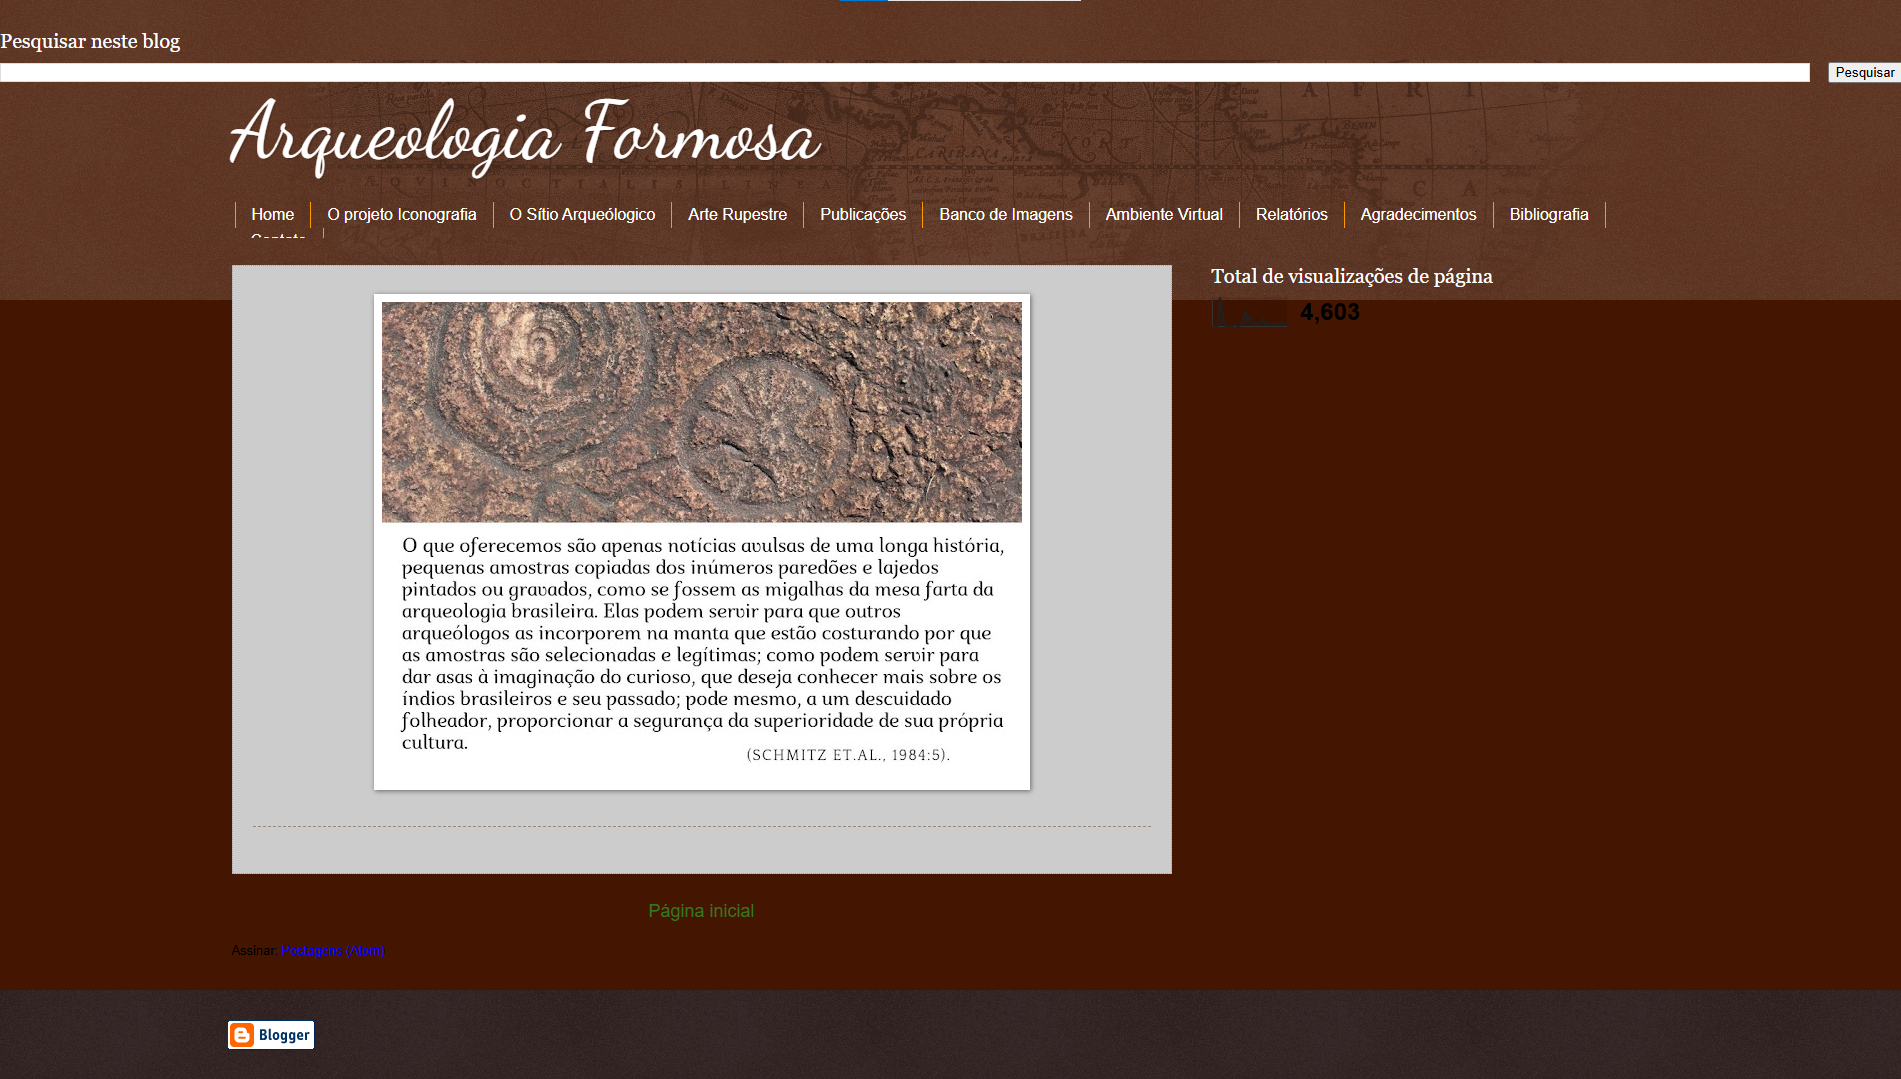
\includegraphics[width=1\linewidth]{images/home-blog-print.png}
    \caption{Captura de tela da página inicial do blog \href{https://arqueologiaformosa.blogspot.com/}{"Arqueologia Formosa"}}
    \label{fig:Captura de tela da página inicial do blog}
\end{figure}

\section{Objetivo Geral}
Desenvolver uma plataforma \textit{web} e um ambiente virtual tridimensional (3D) interativo para preservar, divulgar e democratizar o acesso à arte rupestre da Lapa da Pedra, promovendo a conscientização sobre a importância desses registros culturais para educadores, pesquisadores e o público em geral.

\section{Objetivos Específicos}
Os objetivos específicos do projeto incluem:
\begin{itemize}
    \item Realizar uma análise heurística de usabilidade do antigo site "Arqueologia Formosa", a fim de identificar possíveis melhorias que otimizem a experiência do usuário e garantam uma navegação mais intuitiva e acessível.
    \item Desenvolver um novo site com um design centrado na experiência do usuário, do inglês, \gls{ux}, oferecendo navegação e acessibilidade aprimoradas.
    \item Implementar um ambiente virtual \gls{3d} que permita a visualização interativa da arte rupestre encontrada na Lapa da Pedra e disponibilizar para \textit{download} no site desenvolvido.
    \item Contribuir para a educação patrimonial e a preservação digital do patrimônio cultural da região de Formosa, servindo como modelo replicável para outros sítios arqueológicos.
\end{itemize}


\section{Justificativa}
A relevância deste estudo está intrinsecamente relacionada à crescente importância da Arqueologia Virtual como uma ferramenta eficaz para a preservação e estudo do patrimônio arqueológico em um mundo que enfrenta desafios contínuos em relação à degradação dos sítios históricos. Neste contexto, tecnologias digitais não só oferecem uma nova forma de interagir com o passado, mas também permitem a democratização do acesso a elementos culturais. Por exemplo, projetos semelhantes têm demonstrado que a virtualização de artefatos históricos pode aumentar a conscientização e o respeito pelas culturas que moldaram nossa história.

Por outro lado, a criação de um ambiente digital para a preservação cultural traz inúmeras vantagens tanto para a educação quanto para a pesquisa, possibilitando o acesso a informações e experiências que, de outra forma, seriam limitadas. Além disso, a experiência prévia adquirida pelo autor no PIBIC intitulado "Iconografia e Arte Rupestre Formosense: Criação de um Banco de Imagens e Modelos 3D da Lapa da Pedra" \footnote{Disponível para leitura em: 
\href{https://drive.google.com/file/d/1Id44ViPFScX0Z1TIxGngs4_7UXPabMDt/view?usp=sharing}{https://drive.google.com/file/d/1Id44ViPFScX0Z1TIxGngs4_7UXPabMDt/view?usp=sharing}}, sob a orientação do professor de Artes do  Instituto Federal de Educação, Ciência e Tecnologia de Goiás (IFG), Edson Rodrigues Borges, enriqueceu significativamente a compreensão dos processos de fotogrametria e da criação de modelos 3D aplicados à arqueologia formosense. Com isso, esse conhecimento se torna fundamental para a implementação deste projeto, ao expandir e aprimorar o acesso a esses recursos digitais.

Entre as características do presente trabalho destacam-se: (1) Ambiente virtual interativo, (2) plataforma web com boa usabilidade para documentação dos sítios, (3) visualização dos desenhos em alta resolução a partir dos modelos tridimensionais gerados por fotogrametria e (4) mapa interativo com a localização e informações do sítio da Lapa da Pedra. Na Tabela \ref{tab:comparacao_trabalhos} estão dispostas as características dos trabalhos correlatos e as do presente trabalho:
\begin{table}[h!]
\centering
\resizebox{\textwidth}{!}{%
\begin{tabular}{|>{\raggedright\arraybackslash}m{3cm}|>{\raggedright\arraybackslash}m{2.5cm}|>{\raggedright\arraybackslash}m{2.5cm}|>{\raggedright\arraybackslash}m{2.5cm}|>{\raggedright\arraybackslash}m{2.5cm}|>{\raggedright\arraybackslash}m{2.5cm}|}
\hline
\textbf{Aspectos} & \textbf{\cite{silva2022realidade}} & \textbf{\cite{Magalhães_Berredo_Gaspar_2018}} & \textbf{\cite{pedroignacioschmitz_1984_arte}} & \textbf{\cite{mendonca1977projeto}} & \textbf{Arqueologia Formosa} \\
\hline
\textbf{Área de Aplicação} & Arquitetura & Arqueologia & Arqueologia & Arqueologia & Arqueologia \\
\hline
\textbf{Ambiente Virtual Interativo} & Sim & Não & Não & Não & Sim \\
\hline
\textbf{Site/Plataforma Web} & Não & Não & Não & Não & Sim \\
\hline
\textbf{Mapa Interativo} & Não & Não & Não & Mapa desenhado manualmente & Mapa interativo integrado ao Google Maps \\
\hline
\textbf{Avatar Personalizado} & Avatar personalizado & Não & Não & Não & Avatar personalizado baseado no professor Edson Borges \\
\hline
\textbf{Interatividade} & Alta (navegação em 1ª e 3ª pessoa)  & Baixa (apenas modelos 3D gerados) & Nenhuma & Nenhuma & Alta (navegação em 1ª e 3ª pessoa) \\
\hline
\textbf{Local} & Centro Histórico de Laguna, SC & Sambaqui de Amourins, RJ & Lapa da Pedra, Formosa-GO & Lapa da Pedra, Formosa-GO & Lapa da Pedra, Formosa-GO \\
\hline
\end{tabular}%
}
\caption{Comparação entre os trabalhos correlatos e o presente trabalho.}
\label{tab:comparacao_trabalhos}
\end{table}

Dessa forma, esta pesquisa não apenas contribui para o avanço da Arqueologia Virtual, mas também possui implicações significativas na valorização e proteção do patrimônio cultural. Ao tornar acessíveis as pinturas rupestres da Toca da Onça a um público mais amplo, busca-se não só promover o conhecimento e a apreciação destes tesouros históricos, mas também engajar a sociedade na sua preservação, incentivando a reflexão sobre a identidade cultural e a herança coletiva que todos compartilhamos.

\section{Descrição dos Capítulos}
Os próximos capítulos deste trabalho estão organizados da seguinte forma:
\begin{itemize}
    \item \textbf{Referencial Teórico}
    Dedica-se à fundamentação teórica do trabalho e aos principais conceitos e termos do trabalho, para que o leitor possa ter leitura fluida e compreensão integral do que está lendo. O capítulo aborda sobre a Arqueologia e a arte rupestre, com foco no sítio Lapa da Pedra e nas ameaças à sua preservação. Discute o conceito de patrimônio virtual e suas aplicações, além dos métodos de fotogrametria, modelagem \gls{3d}, e práticas de engenharia de software e desenvolvimento web, com ênfase em Experiência do Usuário. Apresenta também as ferramentas utilizadas.
    
    \item \textbf{Metodologia}: Este capítulo apresenta a metodologia escolhida para o desenvolvimento do projeto, a Design Science Research (DSR), que foi adaptada para cinco fases principais: Identificação do Problema, Definição dos Objetivos da Solução, Design e Desenvolvimento, Avaliação e Comunicação.  A estrutura detalha o processo de identificação do problema e coleta de requisitos.

    
    \item \textbf{Desenvolvimento}: Foca na implementação prática do projeto. Apresenta a construção o desenvolvimento do ambiente virtual na Unreal Engine, detalhando desde a fotogrametria até a disponibilização do executável e, em seguida, o desenvolvimento  do site com Next.js e Sanity. Mostra também os testes realizados e o processo de publicação do site.
    
    \item \textbf{Resultados}: Descreve os produtos finais obtidos, relacionando o cumprimento dos objetivos e trazendo métricas.
    \item \textbf{Conclusão}: Resume os principais resultados alcançados, limitações encontradas e sugestões para trabalhos futuros.
    \item \textbf{Referências}: Lista as obras, artigos e demais fontes bibliográficas consultadas para embasar o trabalho.
    
    \item \textbf{Apêndices}: Apresenta materiais elaborados pelo autor para complementar o trabalho como tabelas, dados brutos, entrevistas, e capturas de telas do sistema.
    
\end{itemize}


    \chapter{Referencial Teórico}
    \label{Referencial_Teorico}
    Este capítulo apresenta o referencial teórico que fundamenta o desenvolvimento do trabalho. Por se tratar de um trabalho com muitos termos técnicos, vale a pena consultar o glossário para uma leitura mais fluida. 
    
    \section{Arqueologia}%
    A Arqueologia é a ciência que estuda as culturas humanas através da recuperação, análise e interpretação dos vestígios materiais deixados por essas sociedades ao longo do tempo. Esses vestígios podem incluir artefatos, edificações, utensílios, entre outros elementos materiais que fornecem informações valiosas sobre os modos de vida, as práticas sociais e as organizações econômicas e políticas dos povos antigos. Conforme destaca \cite{funari2024arqueologia}, a Arqueologia é essencial para a compreensão da história da humanidade, pois complementa e enriquece os dados obtidos por outras disciplinas, como a história e a antropologia, permitindo uma visão mais abrangente e detalhada das sociedades passadas. Assim, ao explorar os vestígios materiais, os arqueólogos contribuem significativamente para a reconstrução e preservação da memória coletiva, além de promover a valorização do patrimônio cultural.
    Ao falar de Arqueologia, podemos nos deparar com várias formas de expressão, como, por exemplo, a arte rupestre.
    \subsection{Arte Rupestre}
    %Falar sobre a definição(que é mais geral), falar sobre a toca da onça. sobre pictoglifos(que são as pinturas).
    
    
    
    O termo “rupestre” tem origem no latim "rupestris”, derivado de “rupes”, que significa "rocha" ou “penhasco”. Assim, define-se como "Arte Rupestre” toda expressão gráfica, seja gravura ou pintura, que utiliza como suporte uma superfície rochosa, independentemente de suas características e dimensões \cite[p. 7]{pedroignacioschmitz_1984_arte}. As paredes de abrigos, grutas, penhascos e até mesmo rochas isoladas se transformam em telas para essas manifestações ancestrais.
    Existem dois principais tipos de arte rupestre:
    \begin{itemize}
    \item \textbf{Pintura Rupestre (Pictografia):} Criação de imagens utilizando pigmentos minerais, vegetais ou animais, aplicados diretamente na superfície rochosa.
    \item \textbf{Gravura Rupestre (Petróglifo):} Produção de desenhos através do desgaste da superfície rochosa, utilizando ferramentas líticas, como pedras pontiagudas.
    \end{itemize}
    A arte rupestre, presente em diversas partes do mundo, representa uma das formas mais antigas de expressão humana, oferecendo informações valiosas sobre as culturas que as produziram (MARQUES, 2016).
    
    \subsection {Sítio Arqueológico Lapa da Pedra}\label{sec:sitio lapa da pedra}
    O Sítio Arqueológico Lapa da Pedra, mostrado na Figura \ref{fig:Entrada da Gruta IV,Toca da Onça}, é conhecido popularmente como Toca da Onça e fica localizado em uma fazenda de propriedade privada a nordeste de Formosa, chamada fazenda Pedra. Na Figura \ref{fig:mapa} pode-se observar o mapa e o caminho percorrido. Em 1984, Pedro Ignácio Schmitz e Altair Sales Barbosa realizaram pesquisas que culminaram na identificação e catalogação de 29 pequenas grutas na região de Formosa, Goiás. Essas grutas abrigavam pinturas rupestres e serviram como moradia para os primeiros habitantes do cerrado (BARBOSA et al., 1984, 1993).
    Dentre as 29 grutas, a Gruta catalogada por Schmitz como IV–GO-EC-002 (04), se destaca pela maior concentração de pictoglifos e, portanto, foi o foco da virtualização neste trabalho. Localizada a cerca de 12 km da cidade de Formosa, a Gruta 04 consiste em uma passagem de duzentos metros abaixo de uma enorme pedra calcária, situada na fazenda Pedra. Esse sítio, semelhante a outros em Goiás e no noroeste de Minas Gerais, apresenta uma grande diversidade de temas na arte rupestre, datando de aproximadamente 4.560 a.C. (SCHMITZ, 1990).
    
    
    \begin{figure}[H]
        \centering
        \includegraphics[height=11cm, keepaspectratio]{img/Entrada Gruta IV Toca da Onça.jpeg}
        \caption{Entrada da Gruta IV, Toca da Onça. \\
            \textbf{Fonte:} Elaborado pelo autor, 2024.}
        \label{fig:Entrada da Gruta IV,Toca da Onça}
    \end{figure}
    
    \begin{figure}[H]
        \centering
        \includegraphics[height=8cm, keepaspectratio]{img/Visitas tecnicas/mapa.png}
        \caption{ Diagrama em cima da captura de tela do Google Earth \\ na localização das grutas da Lapa da Pedra. Captura de tela realizada em junho de 2024 \\
            \textbf{Fonte:} Elaborado pelo autor, 2024.}
        \label{fig:mapa}
    \end{figure}
    
    
    \subsection{Ameaças à Preservação da Arte Rupestre: Deteriorização e Ação Antrópica}\label{sec:amecas a preservação}
    A arte rupestre, como patrimônio cultural de valor inestimável, enfrenta diversos desafios para sua preservação. A ação do tempo e as condições climáticas, como a umidade, a luz, o calor e o vento, contribuem para a deterioração natural das pinturas e superfícies rochosas.
    Na Toca da Onça,  não bate sol dentro da gruta, contribuindo para a preservação do estado dos desenhos. Contudo, ainda se observam fatores de deterioração natural: descamação da tinta, infiltrações, fissuras nas rochas.
    
    
    Além da deterioração natural, a ação antrópica, que se configura como a interferência humana no ambiente, representa uma grave ameaça à preservação da arte rupestre. Vandalismo, turismo desordenado, contato direto com as pinturas, poluição e obras próximas aos sítios arqueológicos podem causar danos irreversíveis a este patrimônio.
    Em relação à Toca da Onça, os seguintes exemplos de impactos causados pela ação antrópica foram notados: vandalismo, pichações, degradação causada pelo turismo desordenado, fotos com \textit{flash}. Como por exemplo o que pode ser observado na Figura \ref{fig:degradacao_toca_onca}.
    
    \begin{figure}[H]
        \centering
        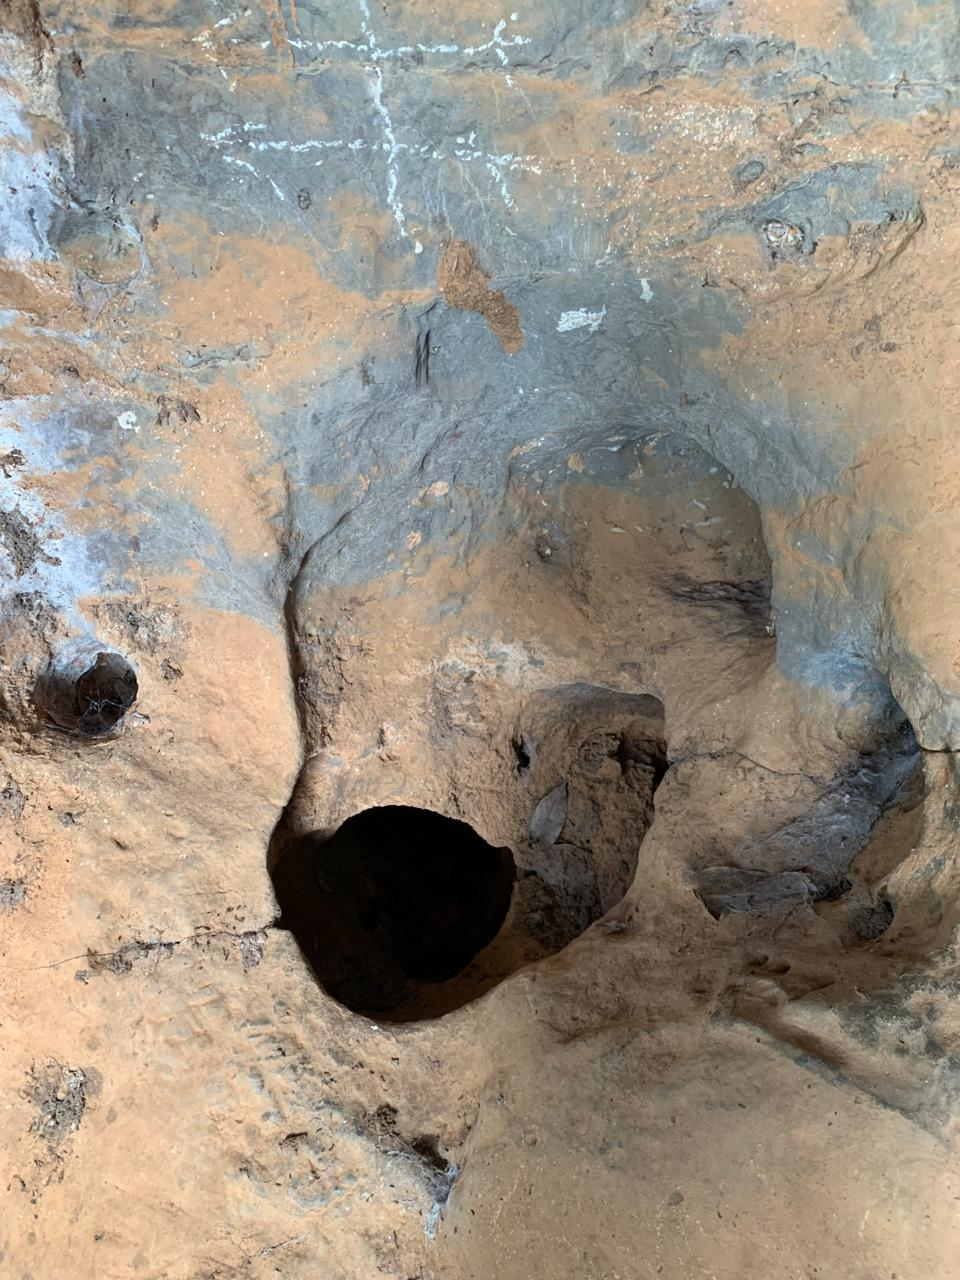
\includegraphics[height=11cm, keepaspectratio]{img/jogo da velha.jpeg}
        \caption{Depredação do Patrimônio na Toca da Onça. \\
            \textbf{Fonte:} Elaborado pelo autor, 2024.}
        \label{fig:degradacao_toca_onca}
    \end{figure}
    
    
    % \section{Patrimônio Virtual (Virtual Heritage)}
    % Discutir o conceito de patrimônio virtual e seu impacto na arqueologia.
    % Diante dos desafios para a preservação da arte rupestre, a virtualização 3D surge como uma ferramenta poderosa para documentar, estudar e divulgar este importante patrimônio cultural, minimizando os impactos causasdos da visitação aos sítios arqueológicos.
    % \subsection{Aplicações em Arqueologia}
    
    
    
    
    \section{Fotogrametria e Modelagem 3D}\label{sec:fotogrametria e modelagem 3D}
    Para construção de um Patrimônio Virtual com qualidade é preciso construir modelos 3D fidedignos a realidade e para isso existe uma técnica muito utilizada chamada fotogrametria.
    A fotogrametria, deriva das raízes gregas “photós” (luz), “gramma” (desenhado ou escrito) e “metria” (medição). Logo, fotogrametria etimologicamente significa “medições gráficas por meio da luz" \citep{Paredes1987}. A American Society for Photogrammetry and Remote Sensing (ASPRS), em seu livro The Manual of Photogrammetry (2003), define fotogrametria como “a arte, ciência e tecnologia de obter informações confiáveis sobre objetos físicos e o ambiente por meio de processos de registro, medição e interpretação de imagens fotográficas e padrões de energia radiante eletromagnética (EM) e outros fenômenos.”
    Historicamente, a fotogrametria  teve seu desenvolvimento intrinsecamente ligado à evolução da fotografia, da óptica e da geometria, culminando em uma ferramenta crucial para diversos campos do conhecimento. No Brasil, sua história acompanha de perto a evolução global, com momentos de pioneirismo e adaptação às demandas nacionais \citep{Silva2013}.
    
    Quanto a sua evolução, a fotogrametria passou por quatro fases principais: a Fotogrametria de Tábua Plana (1850–1900), iniciada por A. Laussedat com o uso de fotografias terrestres para mapeamento; a Fotogrametria Analógica (1900–1950), que incorporou a estereoscopia e fotografias aéreas para fins topográficos; a Fotogrametria Analítica (1950-1990), que otimizou os processos com a introdução de computadores e automatização; e a Fotogrametria Digital (1990-atualmente), caracterizada por processos automáticos realizados em computadores, além da popularização de câmeras digitais de alta qualidade que simplificam o processo \citep{Silva2013}.
    
    A criação de um modelo 3D com fotogrametria digital, como descrito por \cite{silva2022realidade}, envolve um processo que se inicia com o planejamento do levantamento, definindo os objetivos, escolhendo o equipamento adequado e planejando a tomada fotográfica. A etapa seguinte, como apresentado por \cite{groetelaars2004estudo}, é a aquisição de dados no campo, que consiste na captura de fotografias e na medição das coordenadas dos pontos de controle no espaço real, utilizando métodos topográficos ou 3D Laser Scanning. Após a aquisição, o processamento dos dados é realizado por softwares específicos, que orientam as imagens interna e externamente com base nos pontos de controle, gerando uma nuvem de pontos densa. A partir dessa nuvem, o software cria uma malha triangular irregular (TIN), que representa a forma do objeto e pode ser texturizada com as imagens originais. A etapa final envolve o pós-processamento para remover ruídos, \textit{outliers} e falhas, otimizar a malha e aplicar texturas, resultando em um modelo 3D fotorrealístico.
    A fotogrametria automatizada, comumente empregada na geração de modelos 3D de sítios arqueológicos, envolve um processo que se inicia com a captura de imagens de alta qualidade, utilizando câmeras terrestres ou aéreas com sobreposição e georreferenciamento por meio de pontos de controle (GCPs) \citep{McGlone2004}. O software realiza o alinhamento das imagens, corrigindo distorções geométricas e determinando a posição e orientação de cada fotografia no espaço. Através da correlação de imagens, o software identifica pontos correspondentes e calcula as coordenadas 3D de cada ponto, gerando uma nuvem densa de pontos 3D \citep{Heipke2001}. A partir da nuvem de pontos, o software gera modelos 3D, atribui texturas e corrige distorções geométricas, produzindo modelos 3D precisos e realistas do sítio arqueológico \citep{Gruen2008}. A geração de modelos 3D permite a documentação detalhada do sítio, a análise tridimensional da estrutura e a criação de representações visuais para estudos e divulgação científica.
    
    
    %\subsection{Engine}
    \subsection{\textit{Unreal Engine}}No contexto do desenvolvimento de jogos e aplicações interativas, a \textit{engine} desempenha um papel fundamental como a espinha dorsal tecnológica. Uma \textit{engine} de jogo é um conjunto complexo de bibliotecas de software que fornece aos desenvolvedores um arcabouço completo para criar e alimentar experiências interativas em tempo real. Essas ferramentas abrangem desde a renderização gráfica e simulação de física até a inteligência artificial, interface do usuário e gerenciamento de áudio. Sem uma \textit{engine}, os desenvolvedores precisariam construir todas essas funcionalidades do zero, tornando o processo de desenvolvimento significativamente mais complexo e demorado. 
    
    A \textit{Unreal Engine}, desenvolvida pela \textit{Epic Games}, se destaca como uma \textit{engine} de jogos de última geração, amplamente utilizada na indústria de jogos e simulações, e reconhecida por sua capacidade de criar experiências visuais de alta qualidade e interativas.  A \textit{Unreal Engine} oferece um conjunto robusto de ferramentas para modelagem 3D, animação, física, renderização, iluminação, realidade virtual e muito mais. Sua arquitetura flexível e código-fonte aberto permitem que os desenvolvedores personalizem e estendam a \textit{engine} para atender às necessidades específicas de seus projetos, tornando-a uma escolha popular tanto para grandes estúdios quanto para desenvolvedores independentes.
    
    No âmbito do Patrimônio Virtual, a \textit{Unreal Engine} se torna uma ferramenta poderosa para a criação de reconstruções digitais imersivas e interativas de sítios arqueológicos, monumentos e artefatos históricos. A \textit{engine} permite a modelagem 3D realista, a aplicação de texturas detalhadas e a simulação precisa de iluminação, proporcionando aos usuários uma experiência virtual imersiva e próxima da realidade. A capacidade de integrar elementos interativos, como navegação em primeira pessoa, animações e informações contextuais, enriquece ainda mais a experiência, tornando a \textit{Unreal Engine} uma escolha estratégica para projetos que buscam aproximar o público do patrimônio cultural \citep{silva2022realidade}. 
    
    A \textit{Unreal Engine} foi escolhida em detrimento de outras \textit{engines} como a \textit{Unity} e \textit{Godot} pelo fato da facilidade de se construir ambientes realistas.
    
    \subsection{\textit{RealityCapture}  e Integração com \textit{Unreal Engine}}
    O {\textit{RealityCapture}, desenvolvido pela \textit{CapturingReality} e adquirido pela \textit{Epic Games}, é amplamente utilizado para a criação de modelos 3D altamente detalhados a partir de técnicas de fotogrametria. Uma das principais vantagens do \textit{RealityCapture} é sua integração nativa com a \textit{Unreal Engine}, também desenvolvida pela \textit{Epic Games}. Essa compatibilidade facilita a exportação de modelos 3D para a \textit{Unreal Engine}, onde podem ser utilizados na criação de ambientes virtuais realistas, como em jogos, simulações ou experiências de realidade virtual (VR) \citep{EpicGamesDocs}.
    
    A integração entre o \textit{RealityCapture} e a \textit{Unreal Engine} é particularmente útil em projetos de patrimônio cultural, onde a reconstrução digital de sítios arqueológicos ou artefatos pode ser visualizada em ambientes virtuais interativos. Essa combinação permite a criação de experiências imersivas, como visitas virtuais a museus ou sítios históricos, com um alto nível de realismo e detalhamento \citep{silva2022realidade}.
    \subsection{Metahumans}
    
    A representação humana em ambientes virtuais tem papel crucial na criação de experiências imersivas e relacionáveis. No contexto do Patrimônio Virtual, a presença de personagens virtuais humanoides pode auxiliar na comunicação de narrativas históricas, guiar usuários por sítios arqueológicos reconstruídos e demonstrar costumes e atividades do passado. Nesse sentido, a ferramenta \textit{MetaHuman Creator} (Figura \ref{fig:metahuman creator}), da \textit{Epic Games}, surge como um recurso poderoso para a criação de avatares digitais de alta fidelidade.
    O \textit{MetaHuman Creator} permite a geração e personalização de rostos e corpos humanos com alto nível de realismo, incluindo detalhes como cabelo, expressões faciais, textura de pele e diferentes tipos de corpos. A interface intuitiva e a ampla gama de opções de personalização permitem a criação de personagens únicos e específicos, evitando a aparência genérica frequentemente associada a avatares digitais. Esse recurso permite a criação detalhada de personagens realistas que podem ser integrados em simulações e experiências interativas, enriquecendo a representação do patrimônio cultural, tornando-a mais próxima e humanizada.
    
    \begin{figure}[H]
        \centering
        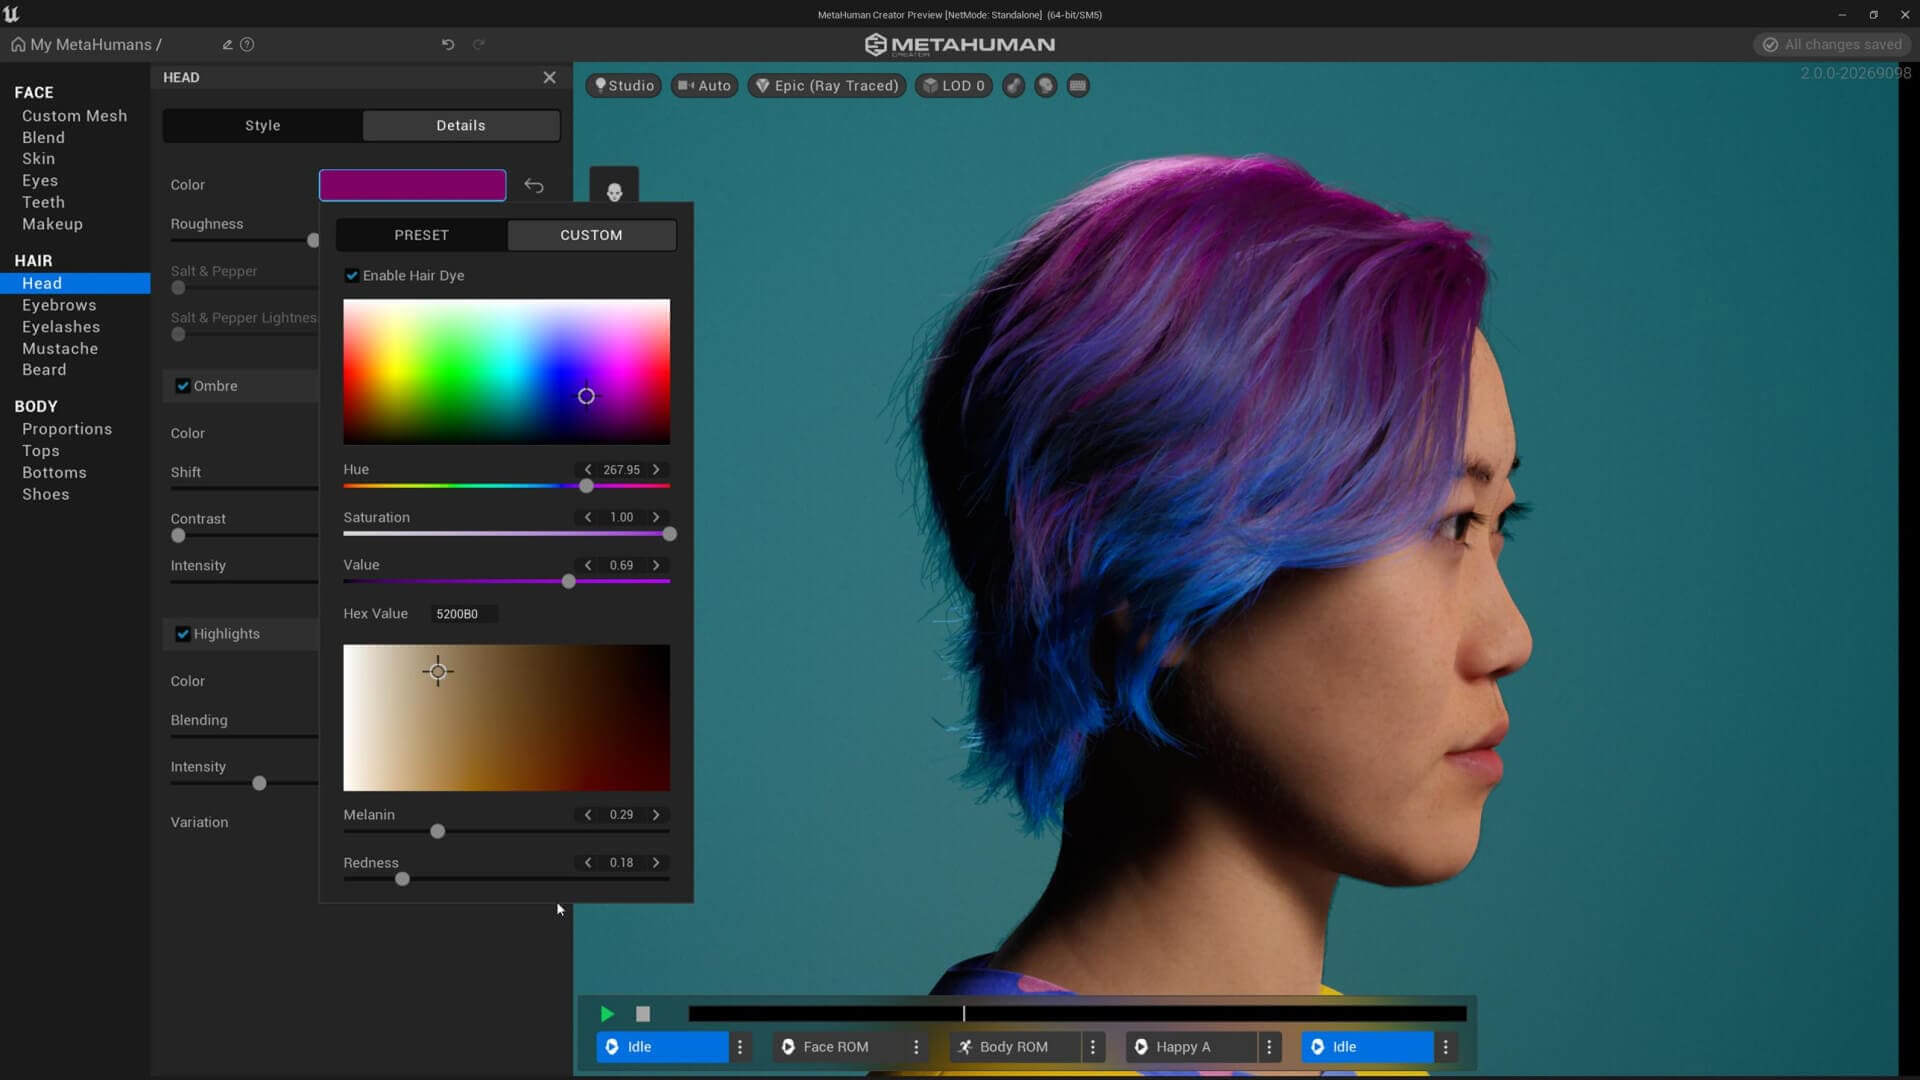
\includegraphics[height=8cm, keepaspectratio]{img/unreal/metahuman create.jpg}
        \caption{Editor da Plataforma \textit{MetaHuman} \\
            \textbf{Fonte:} \href{https://cdn2.unrealengine.com/metahuman-overview-create-1920x1080-baa630fe8b02.jpg?resize=1&w=900}{Unreal Engine - MetaHumans},  \protect\citep{unrealenginemeta}}
        \label{fig:metahuman creator}
    \end{figure}
    
    Um aspecto fundamental para a integração convincente de \textit{MetaHumans} em ambientes virtuais é a animação. Cada \textit{MetaHuman} possui um "esqueleto digital" interno, uma estrutura articulada que permite a aplicação de movimentos, como mostrado na Figura \ref{fig:skeleton}. Através da importação de animações pré-definidas, que podem ser vistas na Figura \ref{fig:animacoes}, ou da criação de animações personalizadas utilizando softwares de animação 3D, é possível atribuir aos \textit{MetaHumans} ações como andar, correr, pular, gesticular e interagir com objetos no ambiente virtual. A fluidez e naturalidade dessas animações são essenciais para garantir a imersão do usuário e a credibilidade da representação.
    
    \begin{figure}[H]
        \centering
        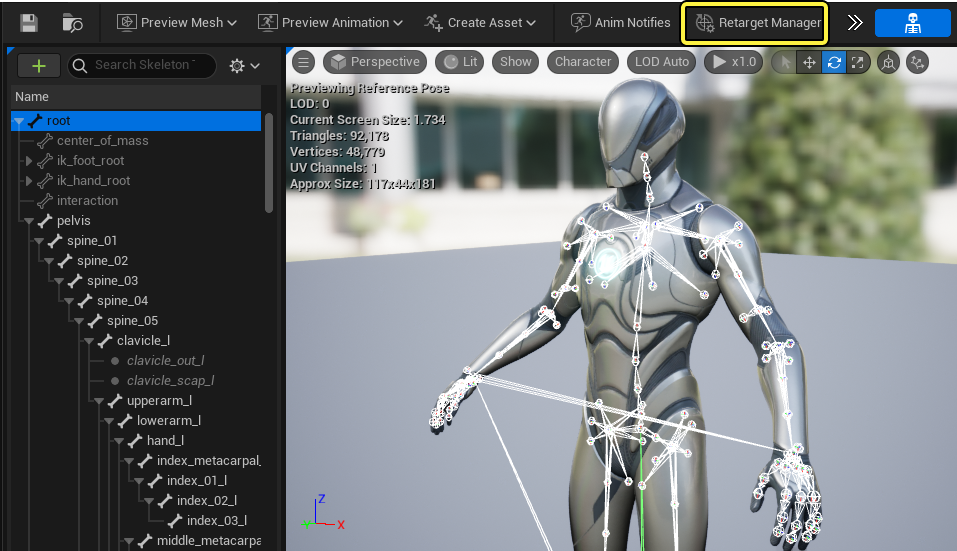
\includegraphics[height=8cm, keepaspectratio]{img/skeleton.png}
        \caption{Captura de tela do Esqueleto digital \\de um avatar na Unreal Engine.\\
            \textbf{Fonte:} Elaborado pelo autor, 2024.}
        \label{fig:skeleton}
    \end{figure}
    
    \begin{figure}[H]
        \centering
        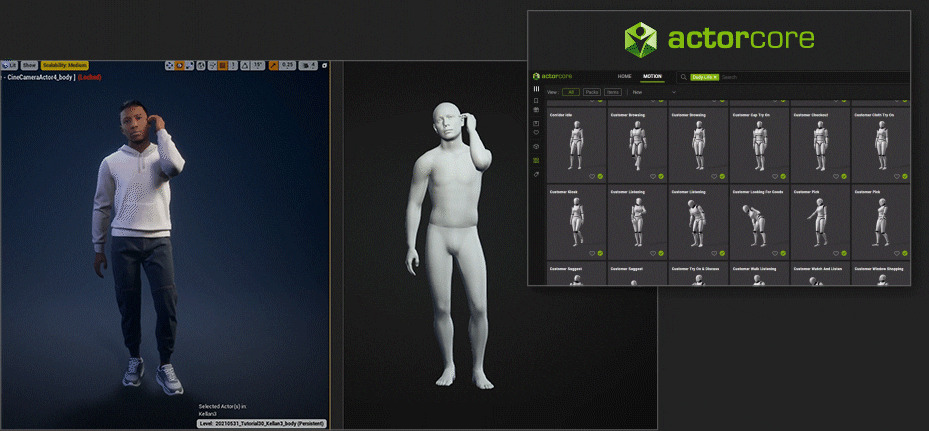
\includegraphics[height=8cm, keepaspectratio]{gif/animacoes/feature_body_motion-0000.jpg}
        \caption{ Captura de tela do pacote de animações Unreal.\\
            \textbf{Fonte:} Elaborado pelo autor, 2024.}
        \label{fig:animacoes}
    \end{figure}
    
    
    A Figura \ref{fig:metahumanEdson} ilustra a aplicação da tecnologia \textit{MetaHuman} na representação do Professor Edson, profissional da área de Artes Visuais e entusiasta da Arqueologia. O modelo digital, criado a partir de fotografias como referência, captura suas características físicas com fidelidade, demonstrando o potencial da ferramenta na criação de representações personalizadas. A utilização de um \textit{MetaHuman} com a aparência do professor Edson Borges em uma experiência de Patrimônio Virtual permite, por exemplo, que ele atue como um guia virtual, conduzindo os usuários por um sítio arqueológico reconstruído, fornecendo explicações e respondendo a perguntas, criando assim uma experiência mais interativa e humanizada.
    
    \begin{figure}[H]
        \centering
        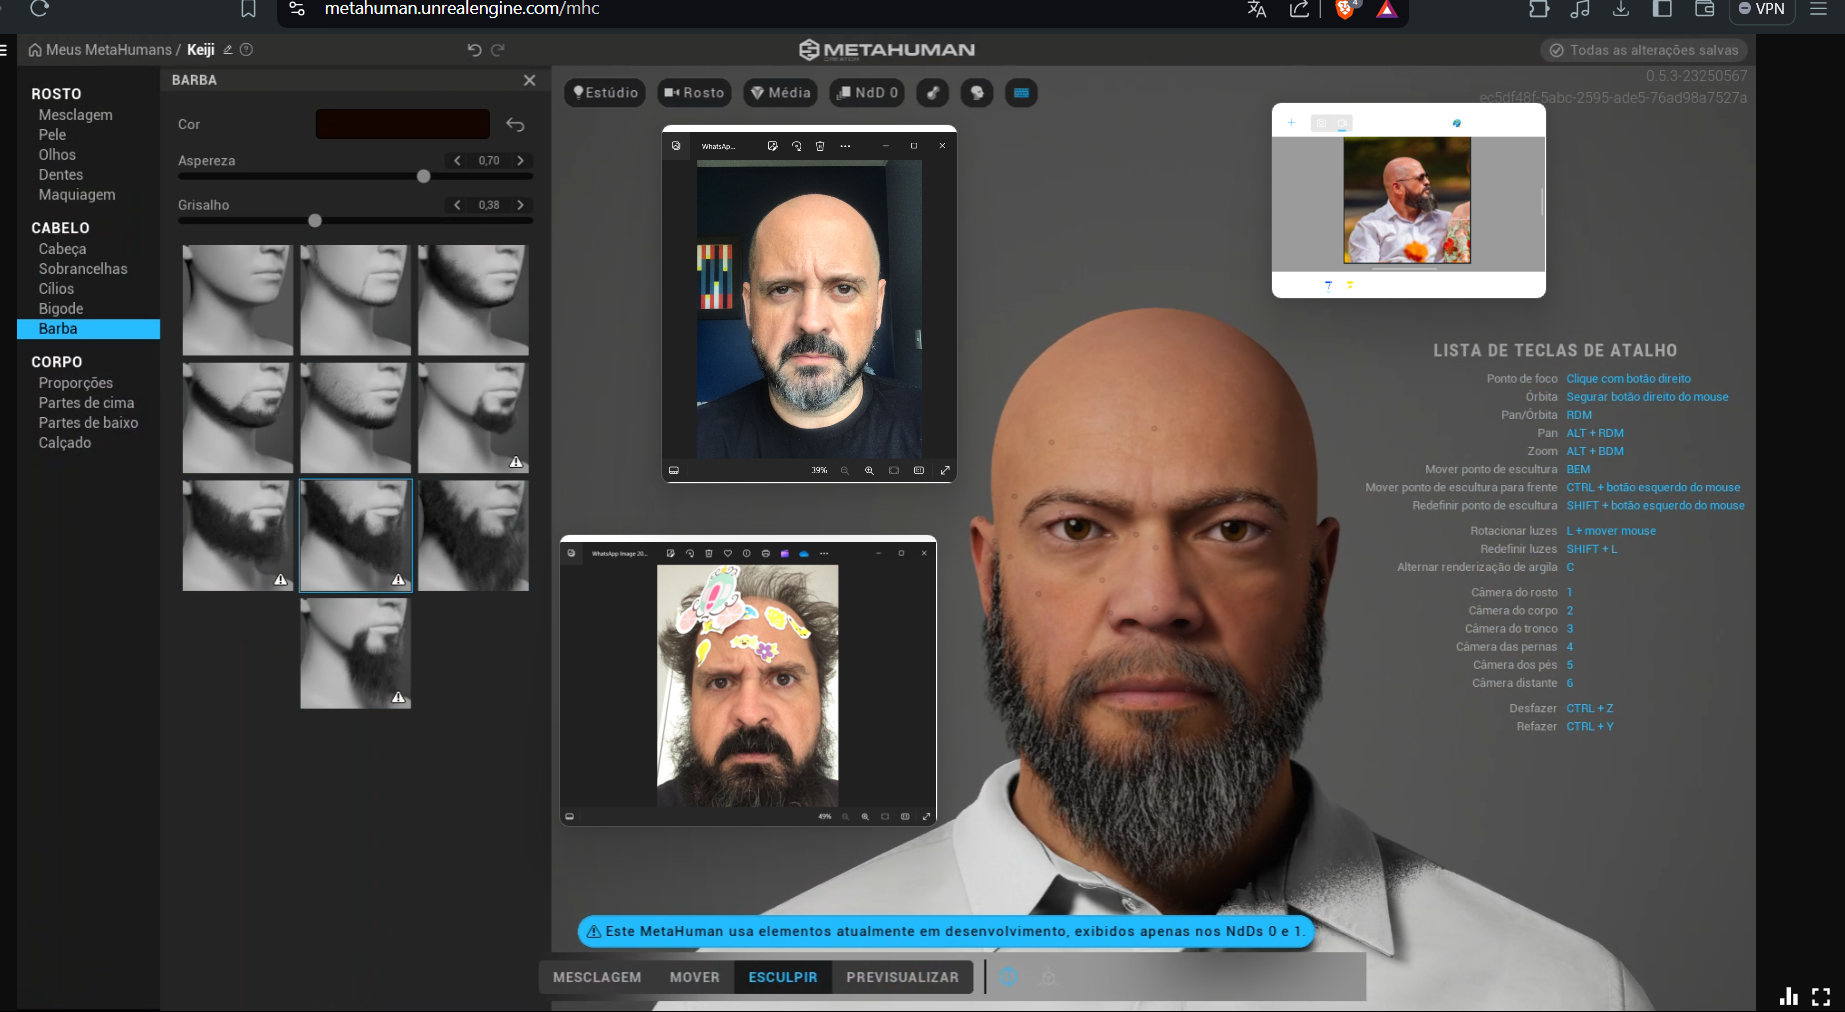
\includegraphics[height=8cm, keepaspectratio]{img/Metahuman.png}
        \caption{Criação do Avatar Digital do professor Edson Borges. \\
            \textbf{Fonte:} Elaborado pelo autor, 2024.}
        \label{fig:metahumanEdson}
    \end{figure}
    
    
    
    A capacidade de gerar personagens virtuais realistas e personalizáveis, combinada com a possibilidade de animá-los de forma natural e convincente, torna os \textit{MetaHumans} uma ferramenta poderosa para a criação de experiências imersivas e envolventes no campo do Patrimônio Virtual. A presença de personagens virtuais humanoides pode contribuir significativamente para a comunicação de narrativas históricas.
    
    \section{Engenharia de Software}
    A engenharia de \textit{software} é um ramo da ciência da computação que se dedica à aplicação sistemática de princípios e práticas de engenharia no desenvolvimento de \textit{software} \citep{pressman2021engenharia}. Seu objetivo primordial reside na criação de sistemas de \textit{software} robustos, confiáveis, eficientes, escaláveis e que atendam às necessidades dos usuários de forma eficaz \citep{Sommerville2011}.
    % \subsection{Modelos de Processo}
    % Discutir diferentes modelos de processo de desenvolvimento de software, como Cascata, Agile, etc.
    
    % \subsection{UML: Unified Modeling Language}
    % A Unified Modeling Language (UML) é uma linguagem de modelagem amplamente utilizada para visualizar, especificar, construir e documentar artefatos de sistemas de \textit{software} \citep{Booch2005}. Criada por Grady Booch, James Rumbaugh e Ivar Jacobson, a UML oferece um conjunto de diagramas padronizados que auxiliam no entendimento e na comunicação entre equipes de desenvolvimento. Segundo \cite{Booch2005}, a UML é composta por diagramas estruturais (como Diagramas de Classe e de Objetos) e comportamentais (como Diagramas de Caso de Uso e de Sequência), que permitem representar diferentes perspectivas de um sistema.
    
    % A UML tem sido fundamental para a engenharia de software, especialmente no contexto de desenvolvimento orientado a objetos. Conforme destacado por \cite{Fowler2005}, a linguagem é flexível o suficiente para ser adaptada a diferentes metodologias de desenvolvimento, como o Rational Unified Process (RUP) e métodos ágeis. Além disso, a UML é mantida e atualizada pela Object Management Group (OMG), garantindo sua evolução contínua para atender às necessidades da indústria de software.
    
    % \subsection{Cenário de Caso de Uso}
    % Um cenário de caso de uso é uma descrição detalhada de uma sequência de interações entre um usuário (ou ator) e um sistema para alcançar um objetivo específico. Esses cenários são fundamentais na engenharia de software, pois ajudam a identificar e esclarecer os requisitos do sistema, garantindo que todas as possíveis interações sejam consideradas durante o processo de desenvolvimento \citep{pressman2021engenharia}.
    
    \subsection{Requisitos Funcionais}
    Requisitos funcionais especificam as funções que um sistema deve executar, descrevendo as entradas, comportamentos e saídas esperadas. Eles definem o que o sistema deve fazer para atender às necessidades dos usuários e são essenciais para orientar o desenvolvimento e a validação do software \citep{pressman2021engenharia}.
    
    \subsection{Requisitos Não Funcionais}
    Requisitos não funcionais referem-se às características de qualidade que o sistema deve possuir, como desempenho, segurança, usabilidade, confiabilidade e escalabilidade. Eles estabelecem restrições e critérios que influenciam a experiência do usuário e a eficácia do sistema, garantindo que o software atenda a padrões de qualidade além das funcionalidades básicas \citep{pressman2021engenharia}.
    
    \section{Desenvolvimento Web}
    
    O desenvolvimento \textit{web} é uma área da tecnologia responsável pela criação, codificação e programação de sites, aplicativos e seus respectivos sistemas, envolvendo tanto aspectos visuais quanto funcionais \citep{queirosintrodução}. Este campo desempenha um papel essencial na democratização do acesso à informação e serviços digitais, permitindo que empresas, instituições e indivíduos alcancem públicos globais por meio da internet.
    
    De acordo com QUEIRÓS E PORTELA (2018), o desenvolvimento \textit{web} pode ser dividido em três áreas principais: \textit{front-end}, \textit{back-end} e \textit{full-stack development}. O \textit{front-end} refere-se à interface do usuário, ou seja, tudo o que o usuário visualiza e interage diretamente no navegador. Já o \textit{back-end} lida com a lógica do servidor, gerenciamento de dados e integração com bancos de dados. O \textit{full-stack development}, por sua vez, combina ambas as áreas, permitindo que um desenvolvedor trabalhe em todas as camadas de uma aplicação web.
    
    No contexto deste projeto, optou-se por utilizar tecnologias modernas que refletem as tendências atuais do desenvolvimento web. Para o \textit{front-end}, foi adotado um \textit{framework} que facilita a criação de interfaces dinâmicas e responsivas\footnote{Responsividade é a capacidade de um site se adaptar a diferentes tamanhos de tela e dispositivos}, melhorando significativamente o desempenho e a otimização para mecanismos de busca, conhecido como \textit{Search Engine Optimization} (SEO). No \textit{back-end}, utilizou-se uma solução de gerenciamento de conteúdo desacoplado (\textit{headless CMS}) que permite maior flexibilidade no design e na entrega de conteúdo, separando a camada de apresentação da camada de dados.
    
    Os autores destacam que o desenvolvimento \textit{web} moderno exige uma abordagem global, considerando tanto os aspectos técnicos quanto a experiência do usuário \citep{queirosintrodução}. Essa perspectiva guiou as escolhas tecnológicas deste trabalho, priorizando desempenho, acessibilidade e facilidade de manutenção.
    
    \section{Experiência do Usuário (UX)}
    A Experiência do Usuário (UX) é um conceito fundamental no design de sistemas interativos, focando na satisfação e na eficiência do usuário ao interagir com um produto ou serviço. Segundo \cite{Norman}, UX abrange todos os aspectos da interação do usuário com uma interface, desde a usabilidade até a experiência emocional.
    
    \subsection{Heurísticas de Nielsen}
    As heurísticas de Nielsen, propostas por Jakob Nielsen em 1994, são um conjunto de princípios amplamente utilizados para avaliar a usabilidade de interfaces. Essas heurísticas servem como diretrizes para identificar problemas de usabilidade e melhorar a interação do usuário. A seguir, são apresentadas as 10 heurísticas de Nielsen:
    
    \begin{enumerate}
        \item \textbf{Visibilidade do Status do Sistema}: O sistema deve sempre manter os usuários informados sobre o que está acontecendo, por meio de feedback adequado e em tempo razoável. Por exemplo, barras de progresso ou mensagens de carregamento são formas de fornecer feedback.
    
        \item \textbf{Correspondência entre o Sistema e o Mundo Real}: O sistema deve falar a linguagem do usuário, com palavras, frases e conceitos familiares, em vez de termos técnicos. As informações devem aparecer em uma ordem natural e lógica.
    
        \item \textbf{Controle e Liberdade para o Usuário}: Os usuários frequentemente realizam ações por engano e precisam de uma "saída de emergência" claramente marcada para sair do estado indesejado. Isso inclui funcionalidades como "Desfazer" e "Refazer".
    
        \item \textbf{Consistência e Padrões}: Os usuários não devem se perguntar se palavras, situações ou ações diferentes significam a mesma coisa. Siga as convenções da plataforma e mantenha a consistência em todo o sistema.
    
        \item \textbf{Prevenção de Erros}: Um bom design evita que problemas ocorram. Isso pode ser feito eliminando condições propícias a erros ou verificando se há erros antes que o usuário confirme uma ação.
    
        \item \textbf{Reconhecimento em vez de Memorização}: Minimize a carga de memória do usuário, tornando objetos, ações e opções visíveis. O usuário não deve precisar lembrar informações de uma parte do sistema para outra.
    
        \item \textbf{Flexibilidade e Eficiência de Uso}: Aceleradores (como atalhos de teclado) podem aumentar a eficiência para usuários experientes, sem prejudicar a experiência de usuários iniciantes.
    
        \item \textbf{Estética e Design Minimalista}: As interfaces não devem conter informações irrelevantes ou raramente necessárias. Cada unidade extra de informação compete com as unidades relevantes e diminui sua visibilidade relativa.
    
        \item \textbf{Ajudar os Usuários a Reconhecer, Diagnosticar e Recuperar-se de Erros}: As mensagens de erro devem ser expressas em linguagem simples, indicar precisamente o problema e sugerir uma solução de forma construtiva.
    
        \item \textbf{Ajuda e Documentação}: Embora seja melhor que o sistema possa ser usado sem documentação, pode ser necessário fornecer ajuda e documentação. Essas informações devem ser fáceis de encontrar, focadas na tarefa do usuário e listar etapas concretas a serem seguidas.
    \end{enumerate}
    
    Essas heurísticas são amplamente utilizadas em avaliações de usabilidade, como inspeções heurísticas, para identificar problemas em interfaces e propor melhorias \citep{Nielsen1994}.
    
    \subsubsection{Análise Heurística}
    A \textbf{Análise Heurística} é um método de avaliação de usabilidade que consiste na inspeção sistemática de uma interface com base em um conjunto de princípios ou heurísticas predefinidas. Esse método é amplamente utilizado para identificar problemas de usabilidade em sites, aplicativos e outros sistemas interativos, sem a necessidade de envolvimento direto dos usuários \citep{Nielsen1994}.
    Os principais objetivos da análise heurística envolvem identificar problemas de usabilidade que possam prejudicar a experiência do usuário; avaliar a conformidade da interface com princípios de design reconhecidos, como as heurísticas de Nielsen; propor melhorias que aumentem a eficiência, a satisfação e a acessibilidade do sistema.
    
    O processo de análise heurística geralmente é composto pelas etapas de:
    
    \begin{enumerate}
        \item \textbf{Seleção das Heurísticas}: Escolha um conjunto de heurísticas adequado ao contexto da avaliação, como as heurísticas de Nielsen.
        
        \item \textbf{Inspeção da Interface}: Um ou mais avaliadores examinam a interface, aplicando as heurísticas selecionadas para identificar problemas de usabilidade.
        
        \item \textbf{Documentação dos Problemas}: Cada problema identificado é documentado, descrevendo sua natureza, a heurística violada e, se possível, sugerindo uma solução.
        
        \item \textbf{Priorização e Relatório}: Os problemas são priorizados com base em sua gravidade e impacto na experiência do usuário, e um relatório detalhado é gerado para orientar as melhorias.
    \end{enumerate}
    
    \subsection{Web Content Accessibility Guidelines (WCAG)}
    
    Outra coisa relacionada com a experiência de usuário é a acessibilidade, e para metrificar isso exitem as \textit{Web Content Accessibility Guidelines (WCAG)}, desenvolvidas pelo W3C, que são padrões globais para acessibilidade digital, garantindo que interfaces sejam acessíveis a todos, incluindo pessoas com deficiências \citep{wcag21}. Organizadas em quatro princípios (\textbf{POUR}), as WCAG abordam:
    
    \begin{itemize}
        \item \textbf{Perceivable (Perceptível)}: Conteúdo deve ser apresentado de forma acessível (ex.: alternativas textuais para imagens).
        \item \textbf{Operable (Operável)}: Interfaces devem ser navegáveis por teclado e compatíveis com tecnologias assistivas.
        \item \textbf{Understandable (Compreensível)}: Conteúdo e operação devem ser claros e previsíveis.
        \item \textbf{Robust (Robusto)}: Conteúdo deve ser compatível com diversas tecnologias.
    \end{itemize}
    
    As WCAG possuem três níveis de conformidade: \textbf{A} (mínimo), \textbf{AA} (recomendado) e \textbf{AAA} (ótimo). Sua adoção promove inclusão digital, conformidade legal e melhoria da experiência do usuário \citep{wcag21}.
    
    % \subsection{Melhores Práticas}
    % Discutir a relevância da acessibilidade, otimização para SEO e práticas comuns de segurança em aplicações web.
    
    
    \section{JAMstack e Desenvolvimento Web Moderno}
    \label{sec:jamstack}
    A JAMstack é uma arquitetura moderna para desenvolvimento \textit{web} que se baseia em três pilares principais: \textbf{JavaScript}, \textbf{APIs} e \textbf{Markup} \citep{jamstackorg}, como exemplificado na Figura \ref{fig:jamStack sigla}\footnote{Disponível em \href{https://cloudbytes.dev/snippets/what-is-jamstack-and-why-should-you-be-using-it}{https://cloudbytes.dev/snippets/what-is-jamstack-and-why-should-you-be-using-it}}. Essa abordagem promove a criação de sites rápidos, seguros e escaláveis, separando o front-end do back-end e utilizando serviços de terceiros para funcionalidades dinâmicas \citep{netlifyjamstack}.
    
    \begin{figure}[H]
        \centering
        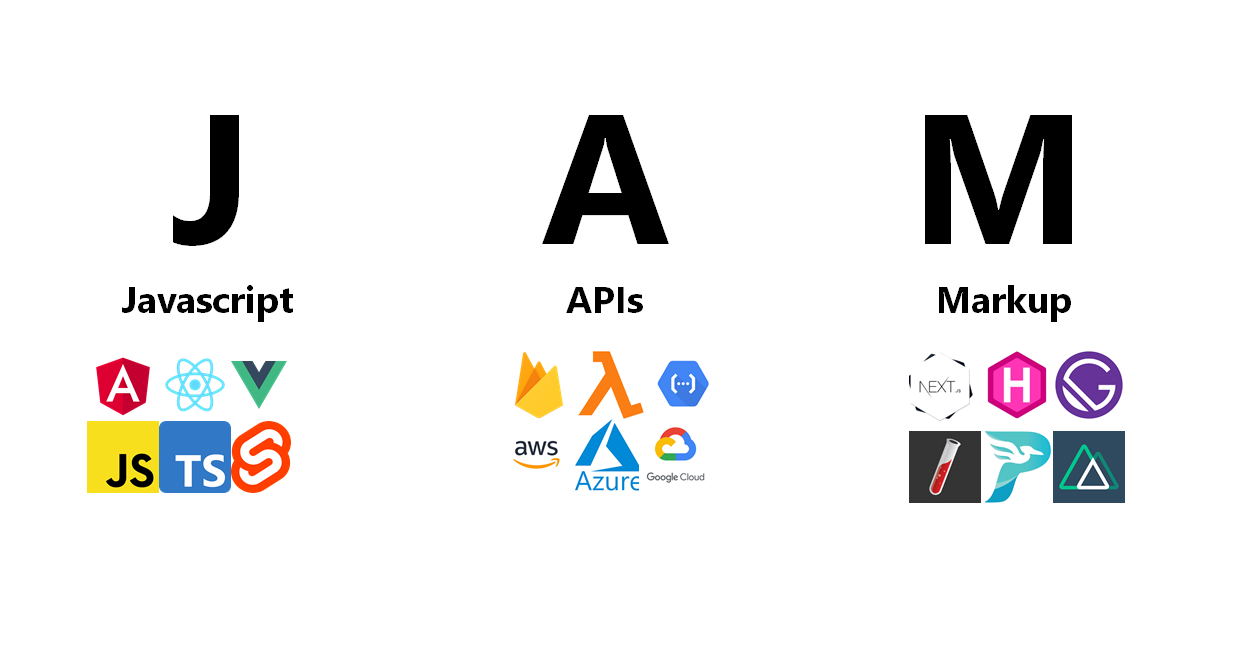
\includegraphics[height=8cm, keepaspectratio]{img/arquitetura/sigla JAM stack.png}
        \caption{ Significado da sigla JAM(Javascript, APIs e Markup)
     \\
            \textbf{Fonte:} Rehan Haider}
        \label{fig:jamStack sigla}
    \end{figure}
    De acordo com \cite{smashingmagazine}, a JAMstack tem ganhado popularidade devido à sua capacidade de simplificar o processo de desenvolvimento, permitindo que desenvolvedores se concentrem na experiência do usuário enquanto delegam tarefas complexas a APIs especializadas. Além disso, a pré-renderização de páginas estáticas contribui para uma melhor performance e segurança, reduzindo a superfície de ataque \citep{jamstackbook}.
    
    A flexibilidade da JAMstack permite a integração com diversas ferramentas e serviços, como CMS \textit{headless}, CDNs e ferramentas de automação, tornando-a uma escolha versátil para projetos de diferentes escalas \citep{netlifyjamstack}.
    
    A arquitetura JAMstack (Figura \ref{fig:jamStack Arquitetura}) se destaca em relação a abordagens mais tradicionais, como o modelo de servidor monolítico e as arquiteturas baseadas em servidores dinâmicos. No modelo monolítico, todo o \textit{back-end} e \textit{front-end} estão fortemente acoplados, exigindo que o servidor processe cada solicitação do usuário em tempo real. Isso pode gerar tempos de resposta mais lentos, especialmente em aplicações com alto tráfego, e torna mais difícil escalar ou implementar novas funcionalidades de maneira isolada.
    
    \begin{figure}[H]
        \centering
        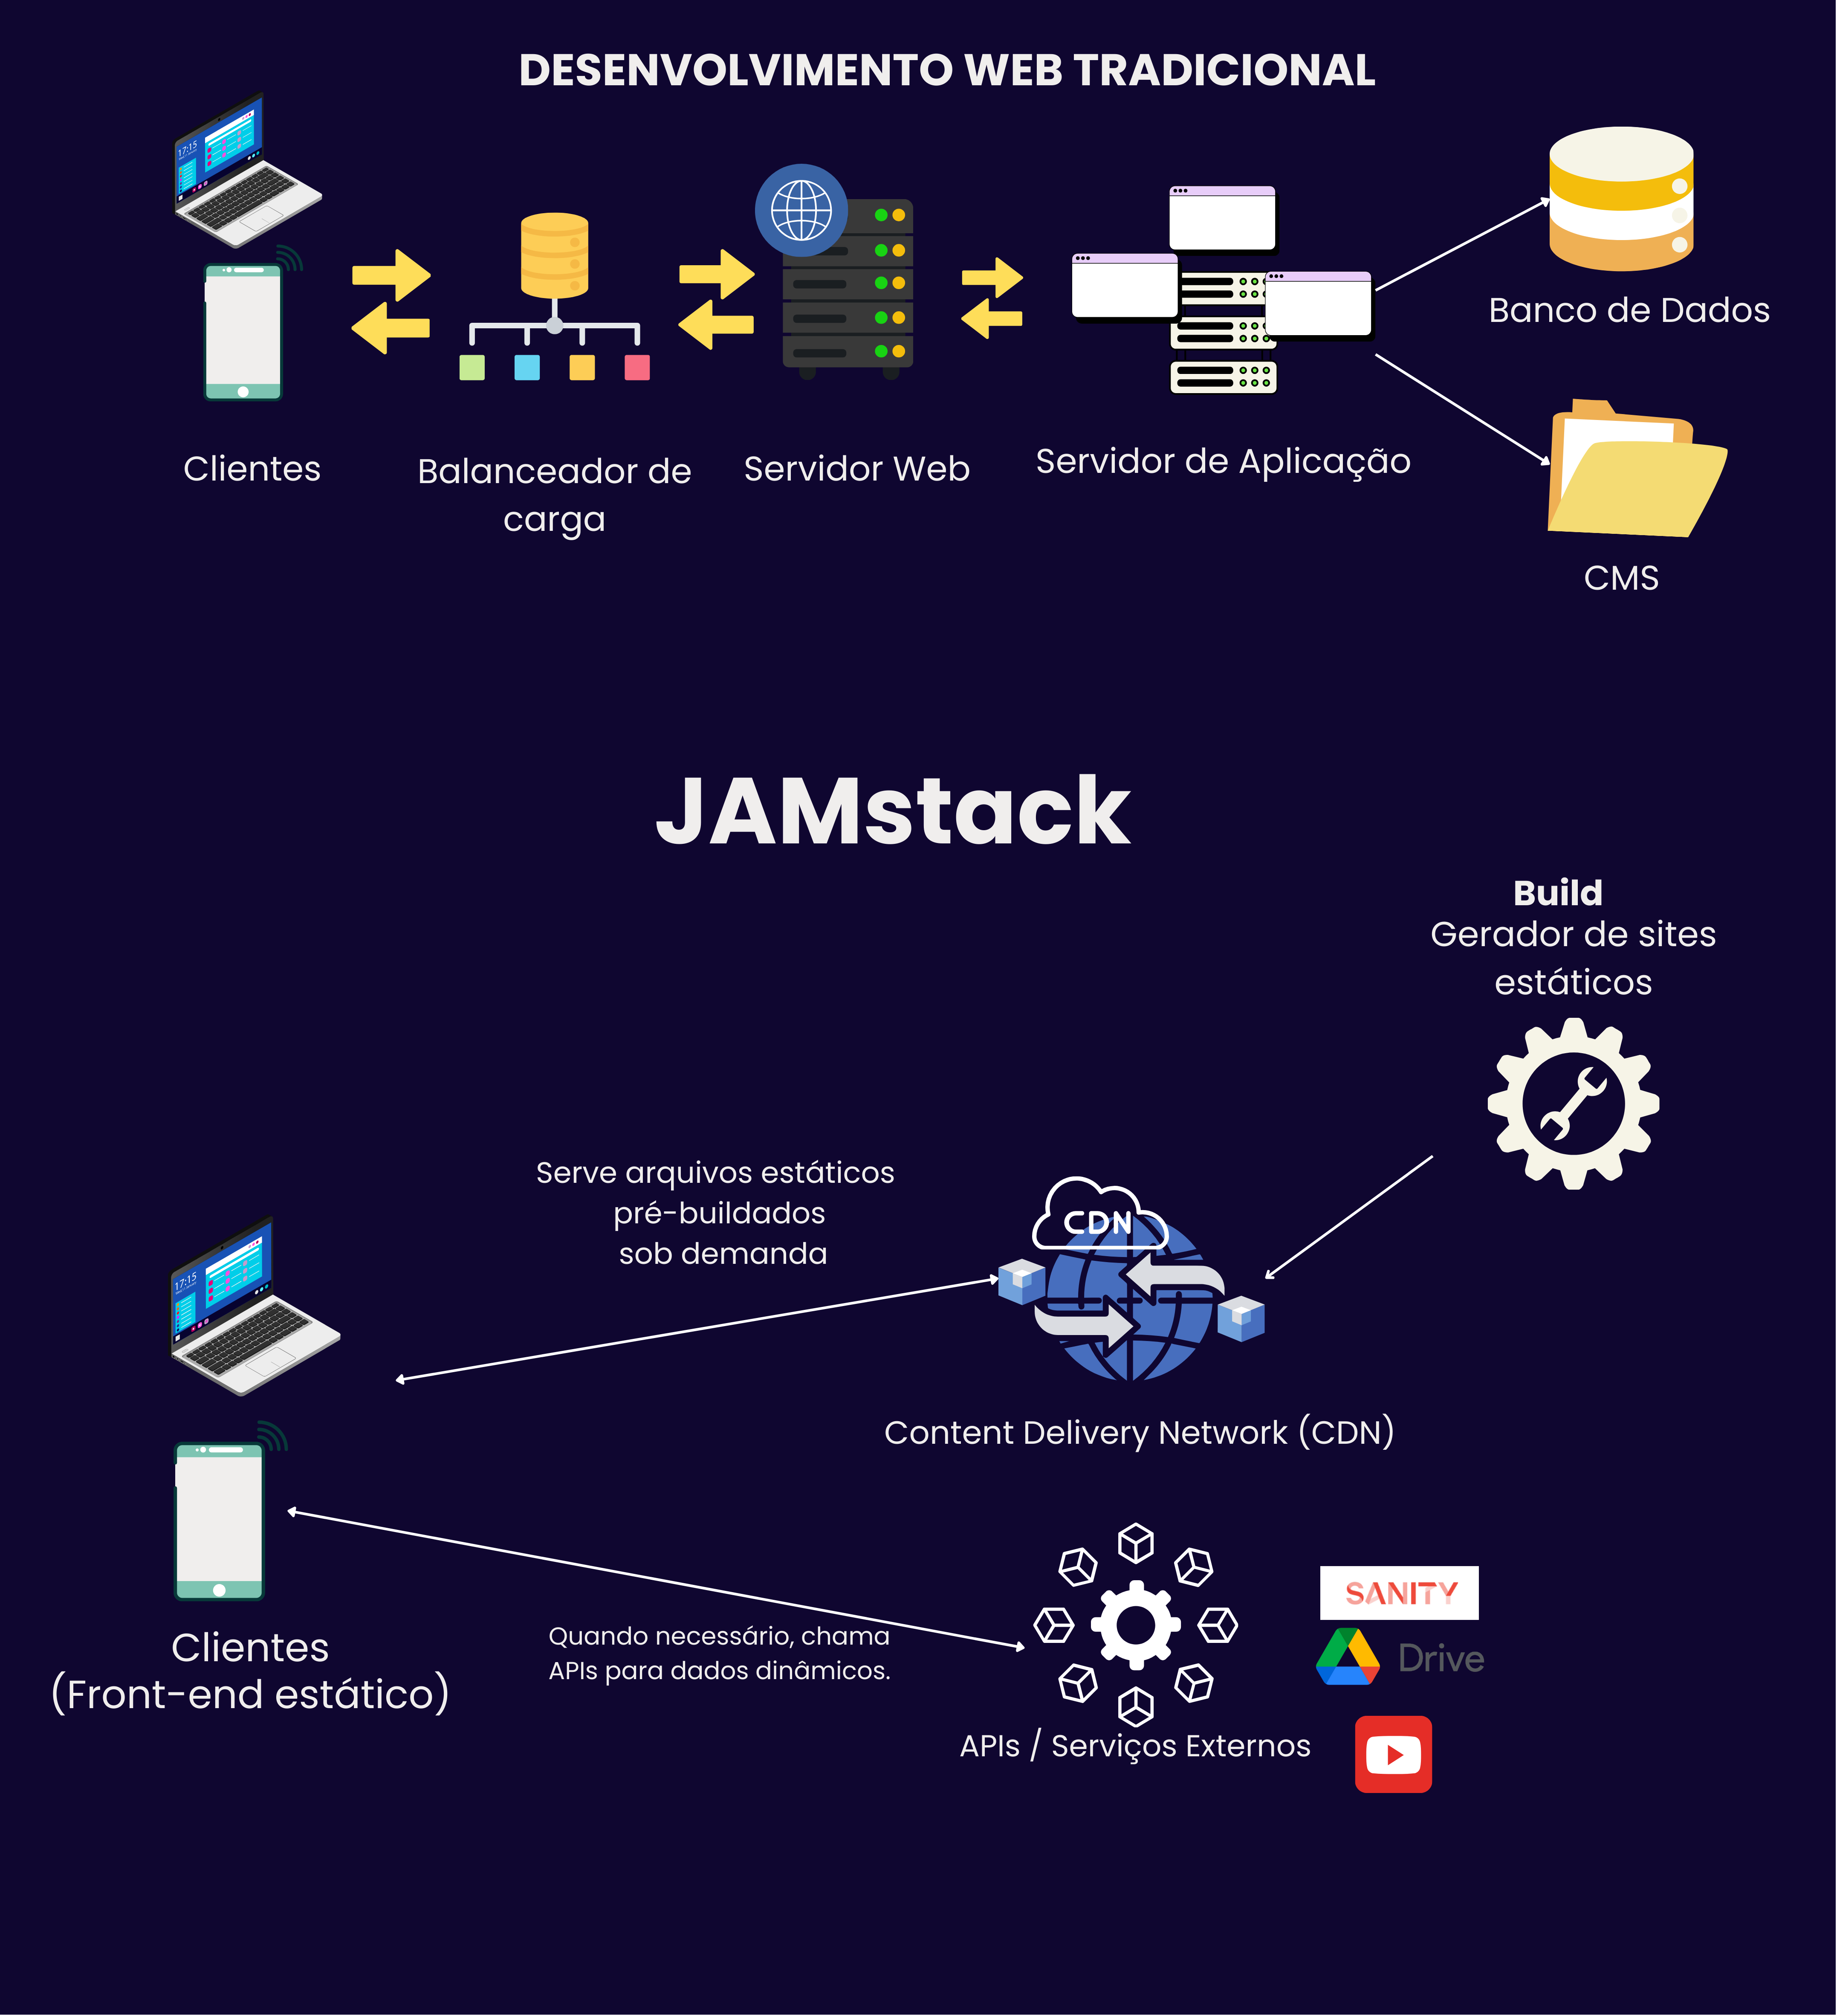
\includegraphics[height=15cm, keepaspectratio]{img/arquitetura/JAMstack explicação.png}
        \caption{ Comparação entre arquitetura tradicional e arquitetura JAMstack. \\
            \textbf{Fonte:} Elaborado pelo autor com base na documentação oficial do JAMstack, 2024.}
        \label{fig:jamStack Arquitetura}
    \end{figure}
    
    Já nas arquiteturas dinâmicas baseadas em servidores, como as utilizadas em sistemas gerenciadores de conteúdo tradicionais (ex.: \textit{WordPress}), cada requisição ao site frequentemente aciona o servidor para buscar dados no banco e gerar a página no momento da requisição. Esse modelo pode causar problemas de performance e segurança, principalmente em picos de tráfego, além de depender de uma infraestrutura robusta para manter a operação.
    Em contraste, a JAMstack evita a necessidade de renderização em tempo de execução, pré-gerando as páginas como arquivos estáticos no momento do \textit{build}\footnote{No contexto da tecnologia, build é o processo de compilar e construir um software a partir do código-fonte. Esse processo envolve a compilação do código e pode resultar em um ou mais arquivos que são considerados prontos para uso.}. Isso garante maior rapidez, segurança e escalabilidade, já que as páginas podem ser servidas diretamente por uma CDN sem passar por servidores intermediários. Além disso, ao desacoplar o \textit{front-end} do \textit{back-end}, a JAMstack permite maior flexibilidade, facilitando a integração com APIs e serviços especializados, como sistemas de pagamento ou autenticação.
    Por outro lado, a JAMstack apresenta limitações quando comparada a arquiteturas como microserviços ou serverless, que também oferecem modularidade e flexibilidade. Embora APIs desempenhem um papel fundamental na JAMstack, aplicações com lógica de negócios altamente complexa podem exigir um \textit{back-end} mais robusto, algo que arquiteturas \textit{serverless} ou baseadas em microserviços conseguem oferecer de forma mais eficiente.
    
    \section{Ferramentas Utilizadas}
    Nesta seção, são apresentadas as principais ferramentas utilizadas no desenvolvimento deste trabalho, destacando suas funcionalidades e relevância para o projeto.
    
    \subsection{Visual Studio Code}
    O \gls{vs-code} é um editor de código-fonte desenvolvido pela Microsoft, amplamente utilizado por desenvolvedores devido à sua leveza, extensibilidade e suporte a diversas linguagens de programação. Ele oferece recursos como depuração integrada, realce de sintaxe, autocompletar inteligente e integração com ferramentas de controle de versão, como Git. Além disso, o VS Code possui um mercado de extensões que permite personalizar e expandir suas funcionalidades, tornando-o uma das ferramentas mais populares para desenvolvimento de software \citep{vscode}.
    
    \subsection{Git e GitHub}
    O Git é um sistema de controle de versão distribuído amplamente utilizado para rastrear alterações no código-fonte durante o desenvolvimento de software. Ele permite que desenvolvedores trabalhem em \textit{branches} separados, facilitando a colaboração e a integração de mudanças. Já o GitHub é uma plataforma baseada em nuvem que hospeda repositórios Git, oferecendo funcionalidades adicionais como \textit{pull requests}, \textit{issues} e integração contínua. Juntos, Git e GitHub formam uma combinação poderosa para gerenciamento de projetos e colaboração em equipe \citep{git,github}.
    
    \subsection{\textit{Notion}}
     Notion é uma ferramenta de produtividade e organização que combina funcionalidades de notas, banco de dados, listas de tarefas e planejamento em uma única plataforma. Ele foi amplamente utilizado neste trabalho para a criação de quadros Kanban \footnote{Kanban é uma ferramenta de gestão visual que utiliza cartões para controlar tarefas e fluxos de atividades, permitindo maior organização e eficiência nos processos. O termo "\textit{Kanban}" significa "sinalização" ou "cartão" e propõe o uso de post-its para indicar e acompanhar o andamento das atividades \citep{aguiar2007compreendendo}} e calendários (Figura \ref{fig:kanban notion}), permitindo o gerenciamento visual de tarefas e o acompanhamento do progresso do projeto. Além disso, o \textit{Notion} foi empregado para o planejamento de etapas, organização de documentação e colaboração em equipe, graças à sua flexibilidade e integração de diferentes tipos de conteúdo em uma única interface. Sua capacidade de personalização e facilidade de uso o tornam uma ferramenta essencial para gestão de projetos e organização pessoal \citep{notion}.
     O \textit{Kanban} nesse trabalho não foi utilizado como metodologia e sim como ferramenta auxiliar. Nele as atividades foram colocadas em um quadro dividido em 4 colunas: Backlog, contendo tarefas planejadas do produto e prioritárias; Não iniciadas, contendo as tarefas a serem feitas; Em progresso, com as tarefas em andamento; Finalizadas, com as tarefas que foram concluídas.
     A Figura \ref{fig:notion inicial} mostra a página inicial usada para organização e planejamento do TCC no \textit{Notion}.
    
    \begin{figure}[H]
        \centering
        \caption{ Página inicial do \textit{Notion} para organização do TCC com etapas, \\ documentos úteis e ferramentas. \\
        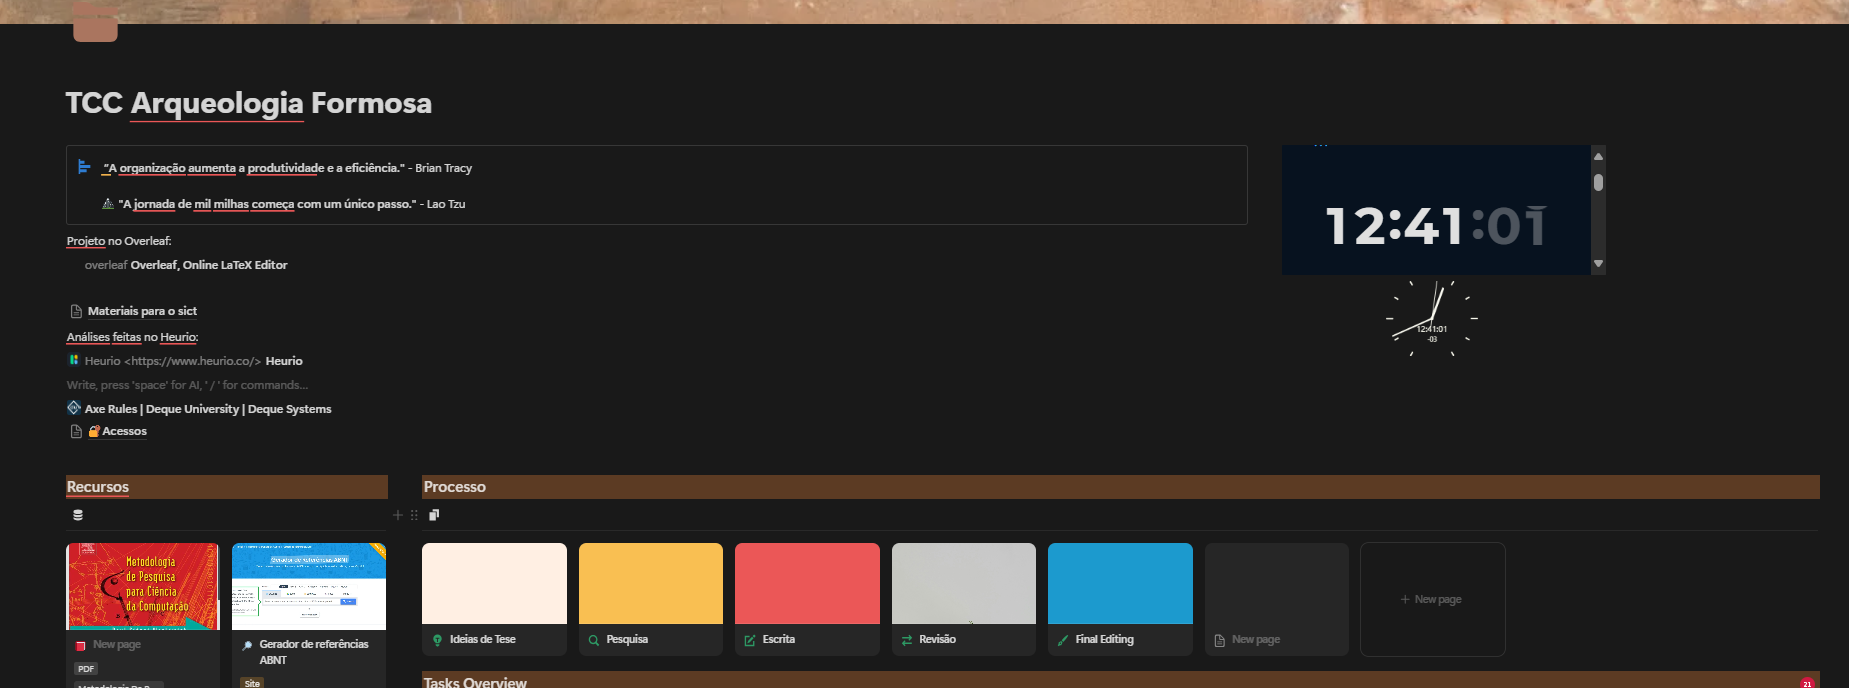
\includegraphics[height=6cm, keepaspectratio]{img/Notion/pagina inicial.png}
            \textbf{Fonte:} Elaborado pelo autor, 2024.}
        \label{fig:notion inicial}
    \end{figure}
    
    \begin{figure}[H]
        \centering
        \caption{ Quadro \textit{Kanban} e calendário para gerenciar atividades. \\
        \label{fig:kanban notion}
        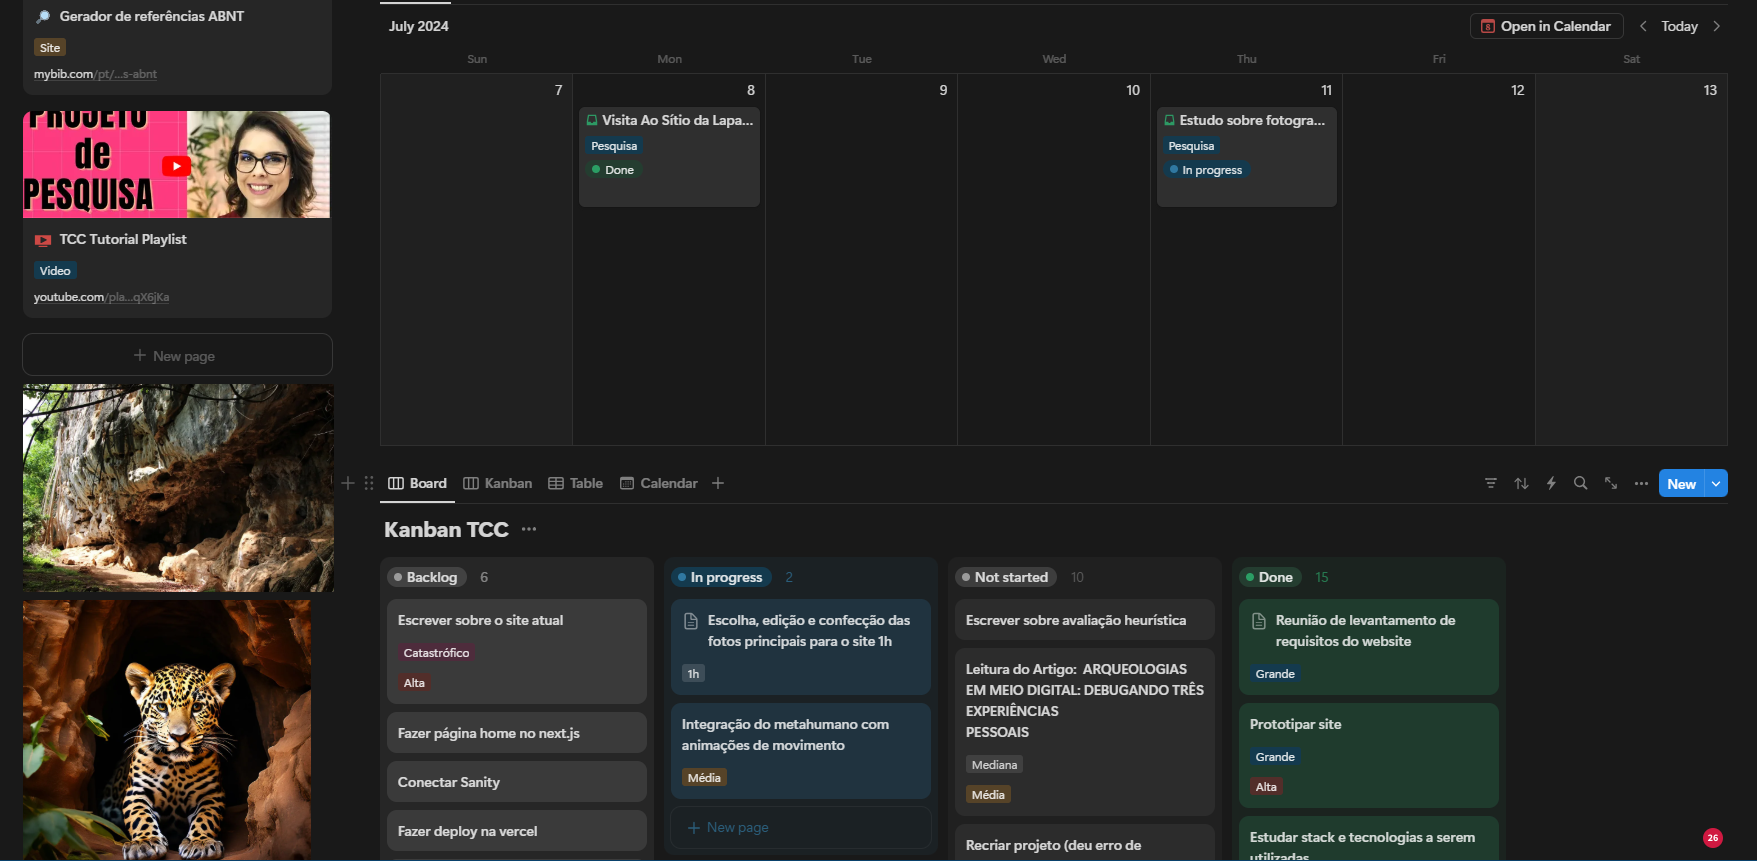
\includegraphics[height=8cm, keepaspectratio]{img/Notion/kanban.png}
            \textbf{Fonte:} Elaborado pelo autor, 2024.}
    \end{figure}

    \begin{figure}[H]
\centering
\caption{Sistema horizontal}  
\centering
\label{fig:horizontal}
\fbox{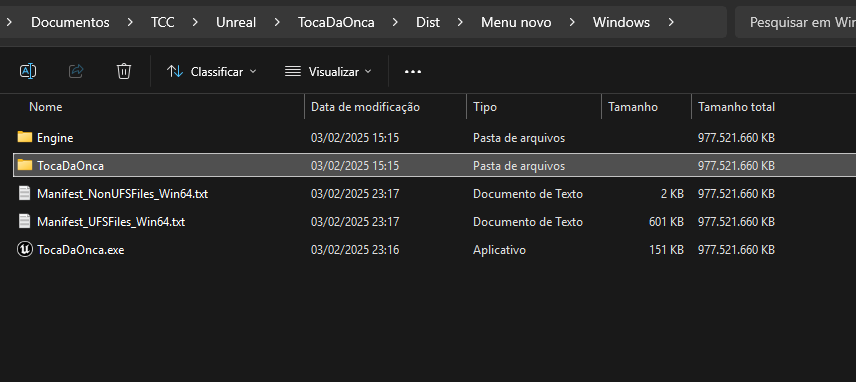
\includegraphics[width=0.78\textwidth, height=0.42\textheight]{img/Inno setup/pastas.png}}
\caption*{Fonte: \cite{de2004astronomia}}
\end{figure}
    
    \subsection{Figma}
    O \textit{Figma} é uma ferramenta de design de interfaces baseada em nuvem, amplamente utilizada para criação de protótipos, designs colaborativos e sistemas de design. Ele se destaca por permitir que múltiplos usuários trabalhem simultaneamente em um mesmo projeto, facilitando a colaboração em tempo real. Além disso, o \textit{Figma} oferece recursos como componentes reutilizáveis, autolayout e integração com outras ferramentas de desenvolvimento, tornando-o uma escolha popular entre designers e equipes de produto \citep{figma}.
    
    % \subsection{Reality Capture}
    % O \textbf{Reality Capture} é uma tecnologia de digitalização 3D que permite criar modelos tridimensionais altamente detalhados a partir de fotografias ou varreduras a laser. Essa ferramenta é amplamente utilizada em áreas como arquitetura, patrimônio cultural, produção cinematográfica e desenvolvimento de jogos, devido à sua capacidade de capturar objetos e ambientes reais com precisão e eficiência \citep{\textit{RealityCapture} 2023}.
    
    % Uma das principais vantagens do Reality Capture é a sua precisão na reprodução de detalhes, o que o torna ideal para projetos que exigem fidelidade ao mundo real. Além disso, a tecnologia é eficiente, permitindo a digitalização de grandes estruturas ou objetos em um tempo relativamente curto. Os modelos gerados podem ser facilmente integrados a softwares de edição 3D e motores de jogos, como o Unreal Engine, o que amplia suas aplicações práticas \citep{\textit{RealityCapture} 2023}.
    
    % No contexto de preservação do patrimônio cultural, o Reality Capture tem sido utilizado para digitalizar monumentos e sítios arqueológicos, garantindo que essas obras sejam preservadas digitalmente para futuras gerações. Na indústria de jogos e filmes, a ferramenta é empregada para criar assets 3D realistas, como personagens e cenários, que podem ser utilizados em produções de alta qualidade \citep{\textit{RealityCapture} 2023}.
    
    % \subsection{Unreal Engine}
    % A \textbf{Unreal Engine}, desenvolvida pela \textit{Epic Games} , é um dos motores de jogo mais populares e versáteis do mercado. Conhecido por sua capacidade de renderizar gráficos de alta qualidade e suportar experiências interativas em tempo real, o Unreal Engine é amplamente utilizado não apenas no desenvolvimento de jogos, mas também em áreas como arquitetura, cinema e educação \citep{UnrealEngine2023}.
    
    % Um dos recursos mais destacados do Unreal Engine é o sistema de \textit{Blueprints}, que permite a criação de lógica de jogo sem a necessidade de escrever código. Isso torna a ferramenta acessível para designers e artistas, que podem prototipar e desenvolver projetos de forma mais ágil. Além disso, o motor oferece suporte a tecnologias avançadas, como iluminação global e física realista, que contribuem para a criação de ambientes visualmente impressionantes \citep{UnrealEngine2023}.
    
    % A integração do Unreal Engine com ferramentas como o Reality Capture é outro ponto forte. Modelos 3D gerados a partir de digitalizações do mundo real podem ser importados diretamente para o motor, onde podem ser manipulados e incorporados em projetos interativos. Essa combinação de tecnologias tem sido amplamente utilizada na criação de jogos realistas, simulações arquitetônicas e até mesmo em produções cinematográficas \citep{UnrealEngine2023}.
    
    % Na área de educação, o Unreal Engine tem sido empregado para desenvolver simulações interativas e ambientes de aprendizagem imersivos. Sua flexibilidade e suporte a múltiplas plataformas, incluindo dispositivos móveis e realidade virtual, tornam-no uma escolha popular para projetos que exigem inovação e engajamento \citep{UnrealEngine2023}.
    
    \subsection{Sanity}
    O \textit{Sanity} é um CMS (\textit{Content Management System}) headless\footnote{ Um Sistema de Gerenciamento de Conteúdo (CMS) é uma ferramenta ou plataforma que permite criar, gerenciar e organizar conteúdo digital, como textos, imagens e vídeos, sem a necessidade de conhecimento técnico avançado. Tradicionalmente, um CMS inclui tanto o \textit{back-end} (onde o conteúdo é criado e armazenado) quanto o \textit{front-end} (onde o conteúdo é exibido). No caso de CMSs \textit{headless}, como o \textit{Sanity}, o \textit{front-end} é desacoplado, permitindo maior flexibilidade na forma como o conteúdo é consumido e apresentado.} que se destaca por sua flexibilidade e arquitetura baseada em \textit{NoSQL}, permitindo a criação de esquemas personalizados e facilitando a entrega de conteúdo em múltiplos canais digitais \citep{sanity_official}. Ele é frequentemente utilizado em conjunto com \textit{frameworks} modernos, como o Next.js, para criar soluções eficientes e escaláveis, onde o \textit{Sanity} atua como \textit{back-end} de conteúdo e o Next.js como \textit{front-end} responsivo e performático. Essa integração reflete uma abordagem contemporânea de desenvolvimento web, alinhada à ideia de sistemas modulares e desacoplados, conforme discutido por \cite{gamma2000padrões} que exploram a evolução das arquiteturas de software, além de funcionar muito bem com a arquitetura JAMstack. 
    
    
    \subsection{Vercel}
    A Vercel é uma plataforma de hospedagem e \textit{deploy} voltada para aplicações modernas, especialmente aquelas construídas com frameworks como \textit{Next.js}, \textit{React} e outros. Ela oferece integração contínua, escalabilidade automática e um desempenho otimizado para aplicações \textit{web} estáticas e dinâmicas. Com foco na experiência do desenvolvedor, a Vercel simplifica o processo de publicação, permitindo que atualizações sejam feitas rapidamente através de integração com \gls{repositorio-git}. Sua infraestrutura global de \glsboth{cdn} garante baixa latência e alta disponibilidade para usuários finais \citep{vercel}.
    
    \subsection{Heurio}
    A extensão Heurio é uma ferramenta desenvolvida para auxiliar na realização de análises heurísticas de sites e interfaces digitais. Disponível como uma extensão para navegadores, o Heurio permite que profissionais de UX apliquem as heurísticas de usabilidade de forma prática e organizada, identificando problemas de usabilidade e propondo melhorias. \citep{Heurio}.
    
    Dentre as funcionalidades do Heurio que facilitam a análise heurística estão:
    
    \begin{itemize}
        \item \textbf{Lista de Heurísticas Integrada}: A extensão inclui uma lista de heurísticas de usabilidade, como as de Nielsen, que podem ser selecionadas e aplicadas diretamente durante a avaliação da interface.
        
        \item \textbf{Anotações e Comentários}: O Heurio permite que o avaliador faça anotações e comentários sobre problemas identificados, associando-os às heurísticas correspondentes. Isso facilita a documentação e a comunicação dos resultados.
        
        \item \textbf{Captura de Tela}: A ferramenta permite capturar telas da interface sendo avaliada, facilitando a visualização e a referência aos problemas encontrados.
        
        \item \textbf{Relatórios Automatizados}: Após a análise, o Heurio gera relatórios automatizados que organizam as anotações, capturas de tela e heurísticas aplicadas. Esses relatórios podem ser exportados e compartilhados com a equipe.
        
        \item \textbf{Colaboração em Equipe}: O Heurio suporta a colaboração entre múltiplos avaliadores, permitindo que equipes trabalhem juntas na mesma análise e compartilhem insights.
    \end{itemize}
    
    Essa ferramenta é particularmente útil em projetos de \textit{redesign} de sites, avaliação de protótipos e testes de usabilidade. Ela pode ser utilizada por equipes de \gls{ux}, designers e desenvolvedores para garantir que as interfaces atendam aos princípios de usabilidade e proporcionem uma experiência positiva ao usuário. Além disso, a ferramenta é flexível o suficiente para ser adaptada a diferentes contextos e metodologias de avaliação. \citep{Heurio}.
    
    \subsection{\textit{Inno Setup}}
    O \textit{Inno Setup} é um instalador gratuito para programas Windows, amplamente utilizado devido à sua facilidade de configuração e flexibilidade. Ele permite a criação de scripts de instalação personalizados, suportando recursos como criação de atalhos, registro de DLLs e desinstalação completa. Sua sintaxe é baseada em arquivos de texto no formato \texttt{.iss}, que são compilados para gerar executáveis de instalação. Por ser leve e de código aberto, o \textit{Inno Setup} é uma escolha popular para desenvolvedores que buscam uma solução eficiente para distribuição de \textit{software} \citep{innosetup}.
\chapter{Metodologia}
\label{cap:metodologia}

O presente trabalho adota a metodologia \gls{dsr}, conforme descrita por \cite{peffers2007design}, que propõe um modelo estruturado para a construção e avaliação de artefatos tecnológicos. A \gls{dsr} é amplamente utilizada em pesquisas de computação e engenharia de software, pois permite a criação de soluções inovadoras baseadas em problemas reais \citep{horita2019design}.

\section{Fases da Design Science Research}

\cite{peffers2007design} definem seis fases principais para a DSR:

\begin{enumerate}
    \item \textbf{Identificação do Problema e Motivação}: Definição do problema e justificativa de sua relevância;
    \item \textbf{Definição dos Objetivos da Solução}: Especificação do que a solução deve alcançar;
    \item \textbf{Design e Desenvolvimento}: Construção do artefato proposto dividida em ciclos;
    \item \textbf{Demonstração}: Aplicação da solução em um contexto real;
    \item \textbf{Avaliação}: Verificação da eficácia da solução.
    \item \textbf{Comunicação}: Divulgação dos resultados para a comunidade científica e profissionais da área.
\end{enumerate}

Neste trabalho, as fases da DSR foram adaptadas para um modelo de cinco etapas, de forma a organizar melhor o fluxo do projeto:

\begin{enumerate}
    \item \textbf{Identificação do Problema};
    \item \textbf{Definição dos Objetivos da Solução};
    \item \textbf{Design e Desenvolvimento};
    \item \textbf{Avaliação};
    \item \textbf{Comunicação}.
\end{enumerate}

Essa adaptação mantém a essência da DSR ao abranger a identificação do problema, definição dos objetivos, construção da solução, avaliação e comunicação dos resultados, garantindo uma abordagem estruturada e alinhada aos objetivos do projeto.

\section{Fase 1: Identificação do Problema}\label{definicao_do_problema}
As abordagens tradicionais de divulgação digital, baseadas em imagens estáticas e textos, limitam a interatividade e a imersão necessárias para explorar sítios arqueológicos. Essa falta de recursos modernos reduz o engajamento do público e dificulta a compreensão espacial desses patrimônios.
No caso do patrimônio arqueológico de Formosa, Goiás, o site original no Blogger desempenhou um papel importante na documentação inicial e na democratização do acesso a pesquisas sobre o Bisnau. No entanto, suas limitações técnicas, como baixa usabilidade, identidade visual desatualizada e restrições de personalização, comprometem a experiência do usuário e o alcance do conteúdo.
Para superar essas limitações, propôs-se o desenvolvimento de um Ambiente Virtual 3D, que permitirá uma exploração imersiva dos sítios arqueológicos e poderá ser baixado pelo novo site. A validação da proposta incluiu:

\begin{itemize}
\item \textbf{Visitas de campo}: Coleta de imagens e informações sobre os sítios, observando deteriorações como pichações e erosão.
\item \textbf{Análise Heurística}: Avaliação do site original com base nas 10 heurísticas de Nielsen, identificando falhas críticas como navegação confusa e falta de acessibilidade.
\end{itemize}

\subsection{Visitas de Campo}
As visitas de campo foram realizadas no sítio arqueológico da Lapa da Pedra, localizado na região nordeste de Formosa, Goiás. Conforme descrito no Referencial Teórico (\ref{sec:sitio lapa da pedra}), o sítio abriga 29 grutas, das quais sete contêm registros de arte rupestre. A Gruta IV S. = Gruta XIV M.–-47.302462,-15.493179 foi o foco principal deste trabalho, sendo a maior e a que contém mais desenhos.

Durante as visitas, observou-se que as pinturas estão distribuídas em alturas variáveis, desde 0,40 metros até 7,50 metros, em superfícies lisas, saliências e reentrâncias naturais do calcário. Apesar de sua relevância histórica, foram identificados sinais de deterioração tanto natural quanto antrópica. Entre os danos naturais, destacam-se a descamação da tinta, infiltrações e fissuras nas rochas, conforme discutido na seção sobre ameaças à preservação (\ref{sec:amecas a preservação}).

Quanto à ação humana, notou-se pichações e escritas superpostas às pinturas originais (Figura \ref{fig:degradacao vera}), reflexo da falta de conscientização sobre a importância cultural do sítio. Esses indícios reforçam a necessidade de estratégias de preservação digital e divulgação ampla, como discutido na Introdução.
\begin{figure}[H]
    \centering
    \includegraphics[height=8cm, keepaspectratio]{img/Visitas tecnicas/depredacao vera.JPG}
    \caption{Escritas superpostas à pinturas original. \\ Está escrito "Vera visitou em 28 de 10 de 62". \\
        \textbf{Fonte:} Acervo pessoal do Ramon Almeida, 2024.}
    \label{fig:degradacao vera}
\end{figure}

Além disso, a localização do sítio em uma propriedade privada, a Fazenda Pedra, contribuiu para sua preservação parcial, mas também limita o acesso e a visibilidade do patrimônio para a população local. Essa constatação evidencia a urgência de iniciativas que promovam a democratização do acesso ao patrimônio cultural, alinhadas ao objetivo deste projeto.

\subsection{Análise Heurística do Antigo Site}
A análise heurística foi realizada no site antigo hospedado na plataforma Blogger com o auxílio da ferramenta Heurio, utilizando como referência as 10 heurísticas de usabilidade propostas por Jakob Nielsen (1994). A análise foi feita por quatro avaliadores: Naoki Rafael Miura, Victor Hugo Sales dos Reis, Sara Candido Fernandes e Erik Takeshi Miura, que identificaram problemas de usabilidade e navegabilidade.
A Figura \ref{fig:interface heurio} mostra a interface do Heurio, enquanto as Figuras \ref{fig:comentario heurio} e \ref{fig:fluxo heurio} mostram o fluxo para inserir as observações da análise, que envolve a identificação do problema, a sugestão de melhoria e a indicação de qual heurística o problema está relacionado.
\begin{figure}[H]
    \centering
    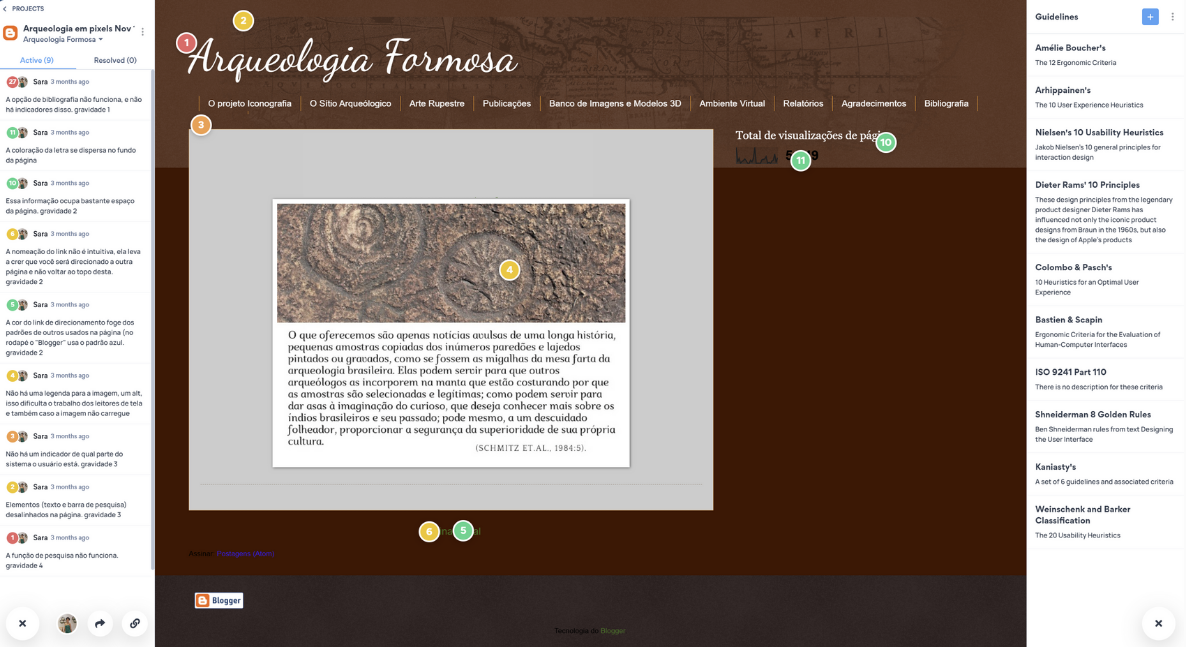
\includegraphics[height=8cm, keepaspectratio]{img/heurio/interface heurio.png}
    \caption{ Interface da ferramenta Heurio. Ela exibe o site a ser analisado, \\ os comentários já feitos no lado esquerdo e os grupos de heurísticas do lado direito. \\
        \textbf{Fonte:} Elaborado pelo autor, 2024.}
    \label{fig:interface heurio}
\end{figure}

\begin{figure}[H]
    \centering
    \includegraphics[height=8cm, keepaspectratio]{img/heurio/habilitar comentários.png}
    \caption{ Botão de habilitar comentários no Heurio.\\
        \textbf{Fonte:} Elaborado pelo autor, 2024.}
    \label{fig:comentario heurio}
\end{figure}

\begin{figure}[H]
    \centering
    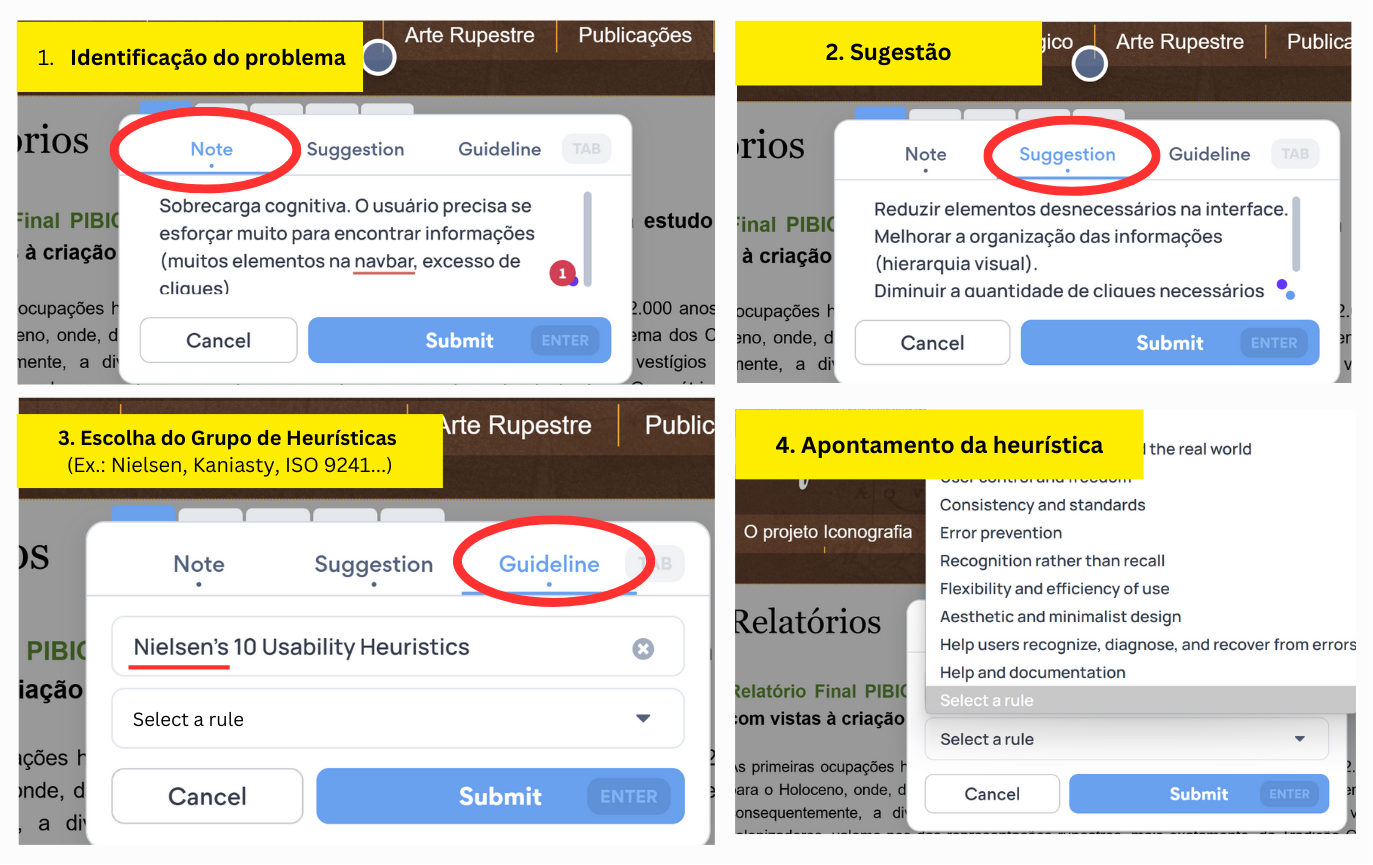
\includegraphics[height=8cm, keepaspectratio]{img/heurio/fluxo heurio.png}
    \caption{ Fluxo de observações incluindo identificação \\do problema, sugestão e heurística relacionada. \\
        \textbf{Fonte:} Elaborado pelo autor, 2024.}
    \label{fig:fluxo heurio}
\end{figure}

% \begin{figure}[H]
%     \centering
%     \begin{minipage}[b]{0.48\textwidth}
%         \centering
%         \includegraphics[height=6cm, keepaspectratio]{img/heurio/habilitar comentários.png}
%         \caption{Botão de habilitar comentários no Heurio.  \\
%             \textbf{Fonte:} Elaborado pelo autor, 2024.}
%         \label{fig:comentario heurio}
%     \end{minipage}
%     \hfill
%     \begin{minipage}[b]{0.48\textwidth}
%         \centering
%         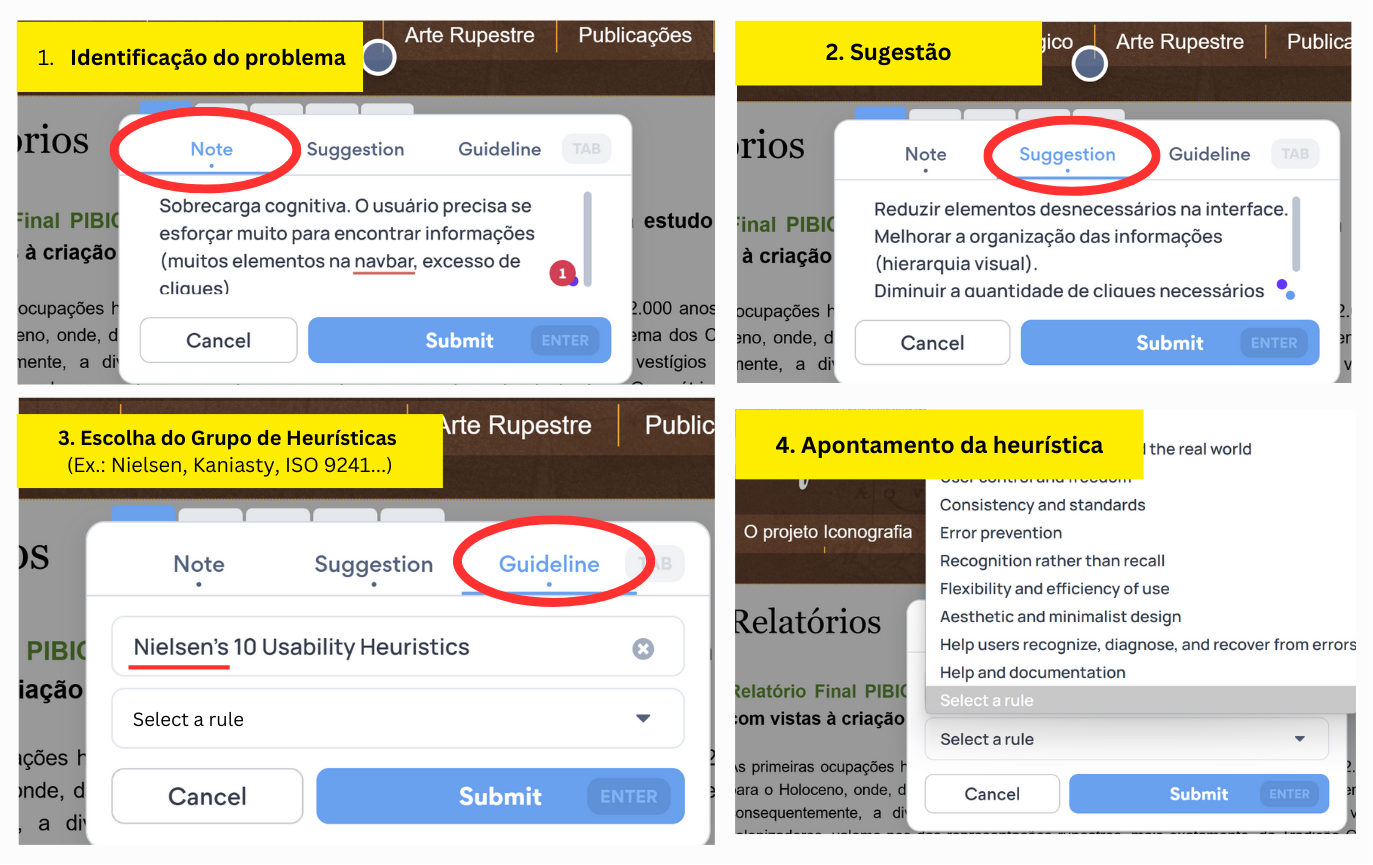
\includegraphics[height=6cm, keepaspectratio]{img/heurio/fluxo heurio.png}
%         \caption{Fluxo de observações incluindo identificação \\do problema, sugestão e heurística relacionada. \\
%             \textbf{Fonte:} Elaborado pelo autor, 2024.}
%         \label{fig:fluxo heurio}
%     \end{minipage}
% \end{figure}

Por fim, a ferramenta Heurio gera um quadro para visualização como se fosse um relatório (Figura \ref{fig:quadro resultados}). Essas observações de cada um dos analistas foram reunidas e contribuíram para a identificação do problema, possibilitando a melhoria do site. 
\begin{figure}[H]
    \centering
    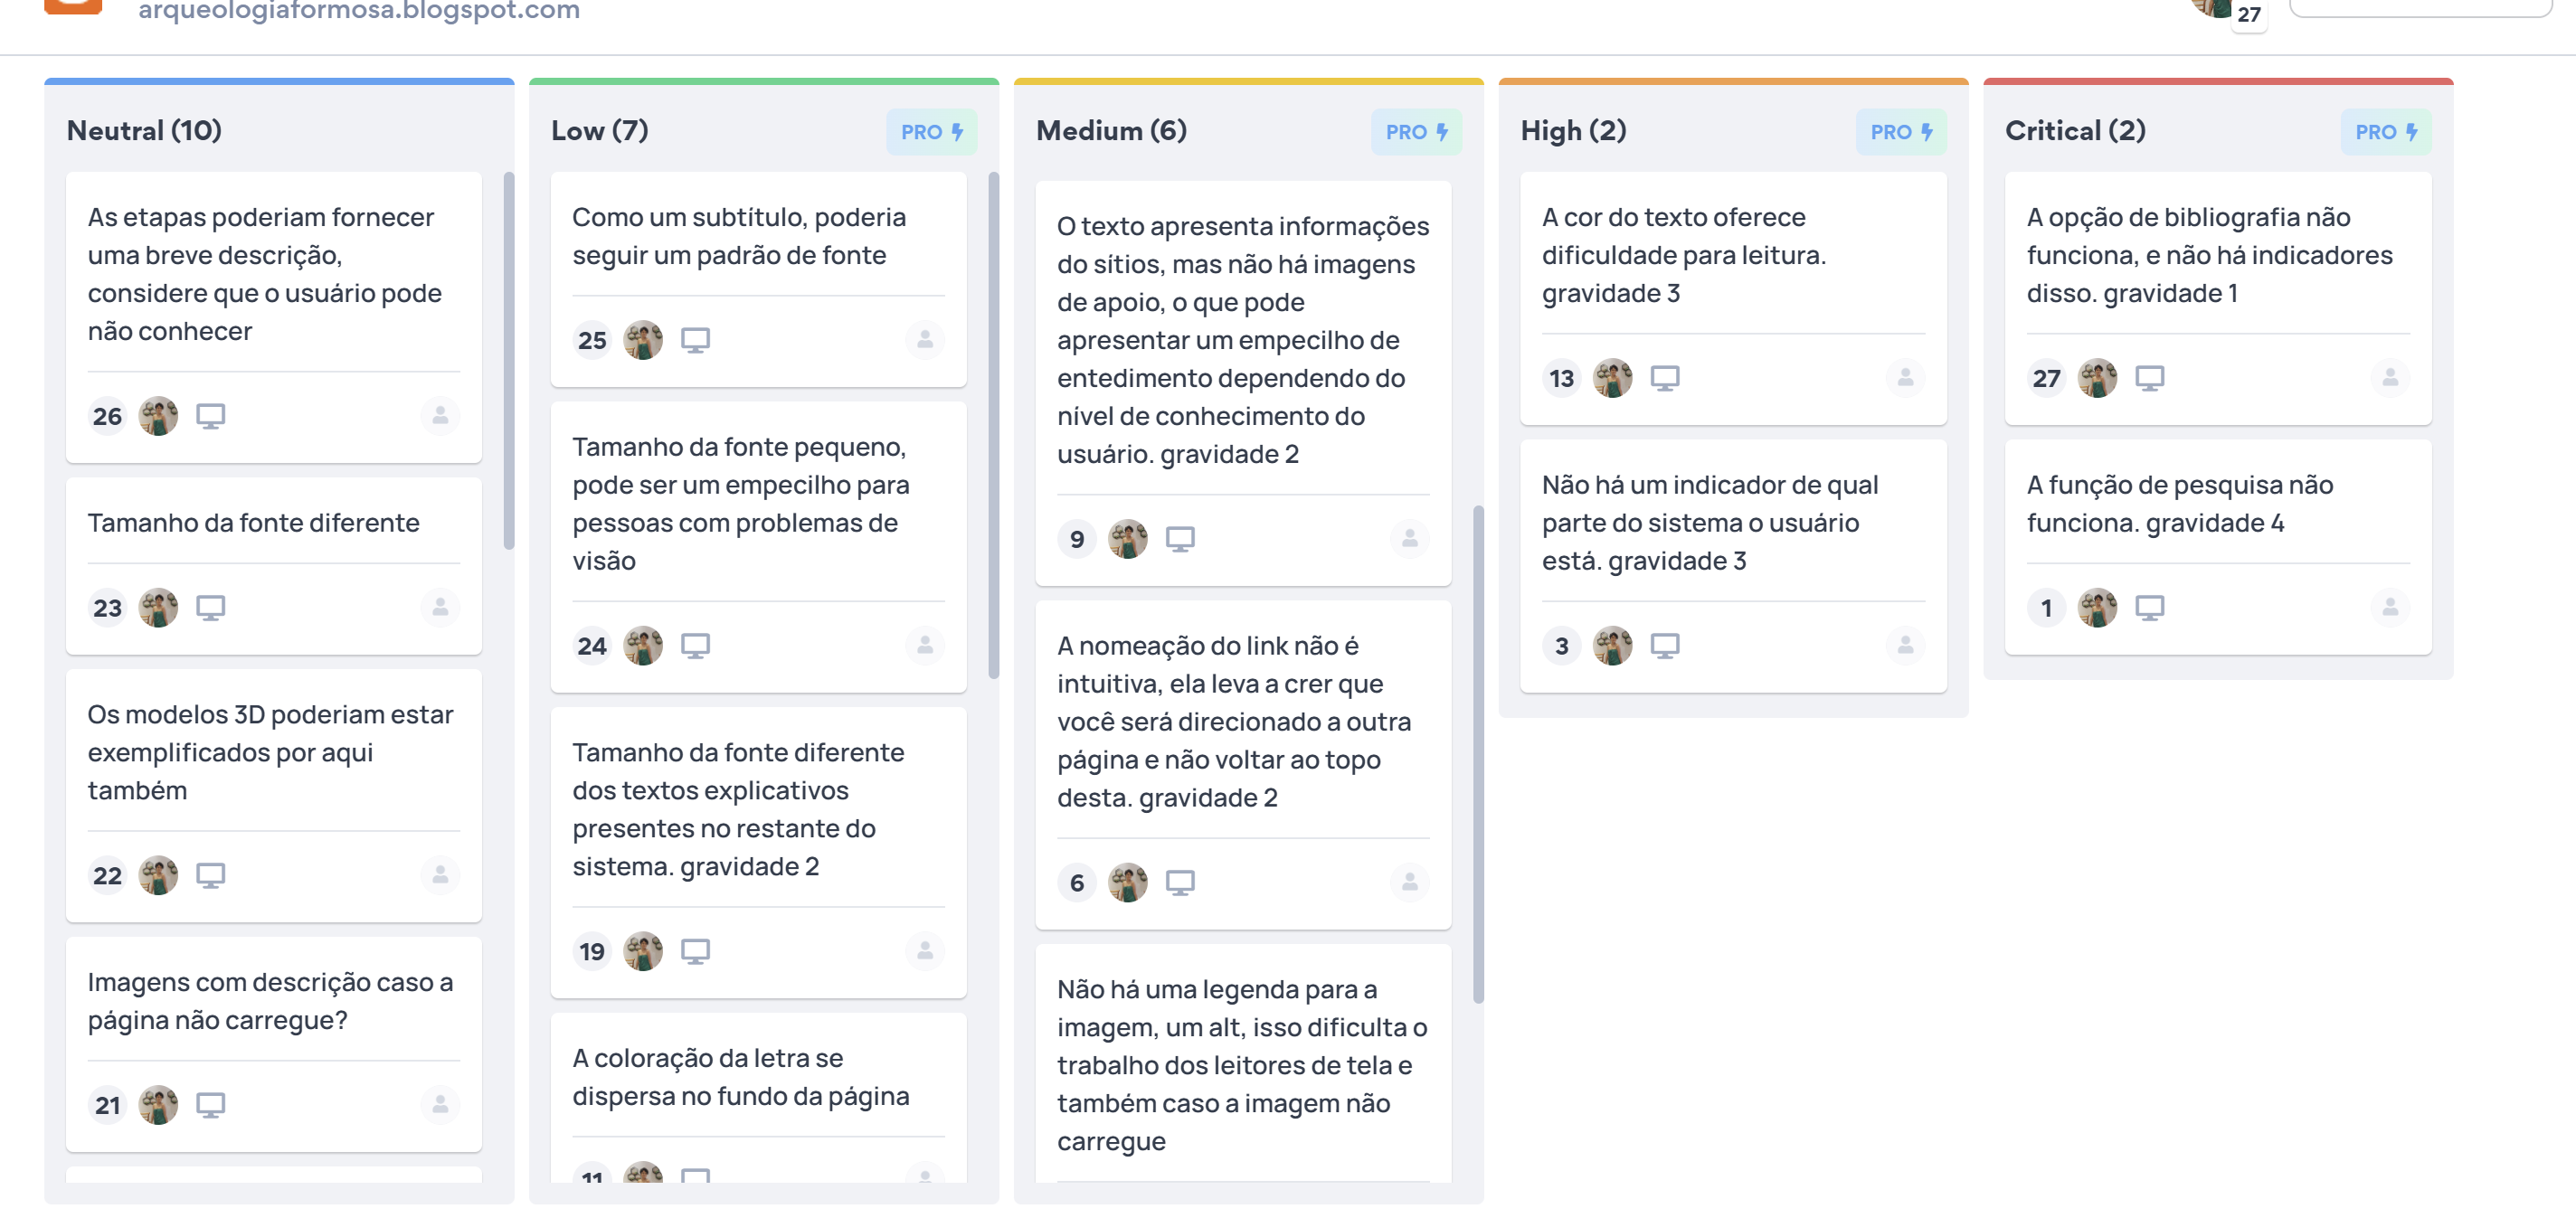
\includegraphics[height=8cm, keepaspectratio]{img/heurio/quadro resultados.png}
    \caption{ Quadro de resultados gerado após a análise do Heurio. \\
        \textbf{Fonte:} Elaborado pelo autor, 2024.}
    \label{fig:quadro resultados}
\end{figure}


\section{Fase 2: Definição dos Objetivos da Solução}\label{definicao_dos_objetivos_da_solucao}
Essa fase envolve a especificação do que a solução deve alcançar. Para isso foi utilizada a técnica de engenharia de requisitos.
\subsection{Coleta de Requisitos}
Coleta de requisitos foi realizada por meio de questionário online e entrevistas formais e informais com professores do IFG, resultando em 13 requisitos funcionais (Apêndice \ref{ap:requisitos-site-table}) e 13 não funcionais (Apêndice \ref{ap:requisitos-nao-funcionais-site-table}) para o site. Para o ambiente virtual há quatro requisitos funcionais (Apêndice \ref{ap:requisitos-ambiente-table}) e 2 requisitos não funcionais (Apêndice \ref{ap:requisitos-nao-funcionais-ambiente}). Todos os requisitos podem ser consultados no apêndice. 

\subsubsection{Identificação dos Requisitos}
\label{sec:identificacao_requisitos}

Por convenção e para facilitar a identificação dos casos de uso junto aos contextos, a referência é feita de acordo com o esquema abaixo:

\textbf{Sigla de subseção | numeração}

Os requisitos são identificados por uma sigla que representa a subseção (por exemplo, "RFS" para Requisitos Funcionais do site, “RNFA” para Requisitos Não Funcionais do Ambiente Virtual) seguida de um número sequencial.

\subsubsection{Prioridades dos Requisitos}
\label{sec:prioridades_requisitos}

Para estabelecer a prioridade dos requisitos, foram adotadas as denominações: essencial, importante e desejável. Abaixo temos a descrição de significado de cada uma dessas denominações:

\begin{table}[H]
\centering
\caption{Prioridades dos Requisitos}
\label{tab:prioridades_requisitos}
\begin{tabular}{|l|p{10cm}|}
\hline
\textbf{Prioridade} & \textbf{Descrição} \\ \hline
Essencial & Requisito sem o qual o sistema não entra em funcionamento. \\ \hline
Importante & Requisito que, sem ele, o sistema entra em funcionamento, mas de forma não satisfatória. \\ \hline
Desejável & Requisito que pode ser deixado para versões futuras sem comprometer as funcionalidades básicas. \\ \hline
\end{tabular}
\end{table}

\subsubsection{Requisitos Documentados}
\label{sec:requisitos_documentados}
{\small 
\begin{longtable}{|p{2.5cm}|p{4cm}|p{6cm}|p{2cm}|}
\caption{Exemplo da Tabela de Requisitos gerada}
\label{table:exemplo_tabela_requisitos} \\
\hline
\textbf{Identificador} & \textbf{Nome} & \textbf{Descrição} & \textbf{Prioridade} \\
\hline
\endfirsthead
\hline
\textbf{Identificador} & \textbf{Nome} & \textbf{Descrição} & \textbf{Prioridade} \\
\hline
\endhead
RFS001 & Exemplo de Nome & Exemplo de descrição do requisito & Essencial, Importante ou Desejável \\ \hline
\end{longtable}
}
Para acessar os requisitos gerados na íntegra, consulte os Apêndices \ref{apendice} e \ref{Apendice B}.


\section{Fase 3: Design e Desenvolvimento}\label{sec: Fase 3 design e desenvolvimento}
Após a identificação do problema \ref{definicao_do_problema} e a definição dos objetivos \ref{definicao_dos_objetivos_da_solucao} da solução, esta seção descreve o processo de design e desenvolvimento do projeto. Seguindo a abordagem da \gls{dsr}, conforme descrita por \cite{peffers2007design}, o desenvolvimento foi estruturado em ciclos iterativos, permitindo refinamento contínuo dos artefatos conforme novas descobertas e avaliações eram feitas.
Neste projeto, os ciclos foram organizados de forma a contemplar as principais etapas do desenvolvimento da solução:

% Ciclo 1
\subsection*{Ciclo 1: Fotogrametria e Construção do Modelo 3D} \label{subsec:ciclo1}

\subsubsection*{Objetivo do Ciclo}
Criar um modelo 3D detalhado baseado em imagens capturadas em campo. Atender ao RFA001 (Modelo 3D de Alta Qualidade) e garantir compatibilidade com \textit{Unreal Engine} 5.4. 

\subsubsection*{Ações Realizadas}
\begin{enumerate}
    \item Captura de imagens de alta resolução de diferentes ângulos do sítio da Lapa da Pedra e seleção para remover fotos com ruídos;
    \item Processamento no \textit{RealityCapture} para reconstrução fotogramétrica, resultando em um modelo inicial com 102 milhões de polígonos;
    \item Simplificação do modelo para 5 milhões de polígonos, garantindo compatibilidade com a \textit{Unreal Engine} (RFA001);
    \item Reprojeção de textura do modelo de alta resolução para o modelo simplificado, mantendo a qualidade visual.
\end{enumerate}

\textbf{Resultado}: Modelo 3D detalhado e otimizado para uso no ambiente virtual, garantindo fidelidade visual e desempenho adequado na \textit{Unreal Engine} 5.4 (RFA001).

% Ciclo 2
\subsection*{Ciclo 2: Construção do Ambiente Virtual na \textit{Unreal Engine} 5.4} \label{subsec:ciclo2}

\subsubsection*{Objetivo do Ciclo}
Atender aos requisitos RFA002 (Navegação em Terceira Pessoa), RFA003 (Alternância de Câmera), RFA004 (Avatar Personalizado), RNFA001 (Compatibilidade com Windows), RNFA002 (Documentação de Instalação) e RNFA003 (Instalação Simplificada).

\subsubsection*{Ações Realizadas}
\begin{enumerate}
    \item Importação do modelo 3D otimizado na \textit{Unreal Engine} 5.4;
    \item Criação do cenário virtual com texturas realistas e iluminação dinâmica;
    \item Implementação do sistema de navegação em terceira pessoa com controle de um avatar interativo (RFA002);
    \item Criação de um avatar personalizado no Metahuman com aparência semelhante ao professor Edson Borges (RFA004);
    \item Desenvolvimento de um sistema de alternância de câmera, permitindo troca entre visão em primeira e terceira pessoa (RFA003);
    \item Configuração de otimizações gráficas para garantir um bom desempenho em máquinas com Windows 10 ou superior (RNFA001);
    \item Empacotamento do ambiente virtual em um arquivo executável (.exe) para distribuição, garantindo instalação simplificada para usuários finais (RNFA003);
    \item Desenvolvimento de um guia de instalação e configuração para orientar os usuários na utilização do ambiente virtual (RNFA002).
\end{enumerate}

\textbf{Resultado}: Ambiente virtual interativo e otimizado, permitindo exploração em terceira pessoa com opção de alternância para visão em primeira pessoa, avatar personalizado, compatibilidade com Windows 10+ e um instalador simplificado para facilitar a distribuição e configuração pelos usuários finais (RFA002, RFA003, RFA004, RNFA001, RNFA002, RNFA003).

% Ciclo 3
\subsection*{Ciclo 3: Prototipação do Novo Site} \label{subsec:ciclo3}

\textbf{Objetivo do Ciclo}: Desenvolver um protótipo o novo site, atendendo aos requisitos funcionais RFS002 (Exibir Galeria de Imagens), RFS006 (Buscar Trabalhos por Filtros) e RFS007 (Informações de Contato), bem como aos requisitos não funcionais RNFS006 (Acessibilidade), RNFS008 (Responsividade) e RNFS012 (SEO).

\subsection{Ações Realizadas}
\begin{enumerate}
    \item Análise das referências e inspirações enviadas pelo professor Edson Borges por meio de um questionário.
    \item Reorganização da arquitetura da informação, agrupando conteúdos relevantes e reduzindo cliques (RNFS006).
    \item Criação de wireframes para estruturar a interface e definir a disposição dos elementos visuais (RNFS008).
    % \item Definição da paleta de cores e tipografia, garantindo coerência visual e acessibilidade (RNFS006).
    \item Criação de uma nova logo, inspirada nas cores das artes rupestres da Lapa da Pedra.
    \item Desenvolvimento de um protótipo de alta fidelidade no Figma, representando a versão final do site.
    \item Validação e refinamento do protótipo a partir de feedbacks coletados com o professor e colegas.
    \item Organização eficiente do projeto no Figma, facilitando futuras iterações e implementações.
\end{enumerate}

\textbf{Resultado}: Protótipo de alta fidelidade bem estruturado e validado, garantindo acessibilidade, melhor navegação, identidade visual consistente e um layout flexível para futuras alterações e desenvolvimento (RNFS006, RNFS008, RNFS014).
% 4
\subsection*{Ciclo 4: Desenvolvimento do Novo Site} \label{subsec:ciclo4}

\subsubsection*{Objetivo do Ciclo}
Atender aos requisitos funcionais e não funcionais do site. O desenvolvimento abrange a maioria dos requisitos especificados nas tabelas \ref{ap:requisitos-site-table} e \ref{ap:requisitos-nao-funcionais-site-table}, garantindo acessibilidade, responsividade, gerenciamento dinâmico de conteúdo e otimização de desempenho.

\subsubsection*{Ações Realizadas}
\begin{enumerate}
\item \textbf{Configuração do ambiente de desenvolvimento}: Definição da arquitetura \textit{JAMstack}, utilizando o \textit{framework} \textit{Next.js} e a biblioteca \textit{Schema UI} no \textit{front-end} e \textit{Sanity} como CMS headless, além da configuração do repositório no Git e escolha da hospedagem na Vercel para otimização de desempenho e redução de custos (RNFS001, RNFS008, RNFS011).

    
    \item \textbf{Implementação da estrutura e funcionalidades do site}
    \begin{enumerate}
        \item Implementação de páginas-chave:
        \begin{enumerate}
            \item Página inicial com navegação hierárquica
            \item Seções específicas para sítios arqueológicos
            \item Página de Contato
            \item Página de trabalhos escritos com filtros
        \end{enumerate}
    \end{enumerate}
    
\end{enumerate}

\section{Fase 4: Avaliação} \label{sec:avaliacao-dsr}

    \textbf{Validação Técnica}
    \begin{enumerate}
        \item Testes de performance com Lighthouse;
        \item Verificação de compatibilidade em 6 navegadores diferentes;
        \item Avaliação heurística do novo site e \textit{feedbacks}.
    \end{enumerate}
    

\section{Fase 5: Comunicação} \label{sec:comunicacao-dsr}

Os resultados foram divulgados através de:
\begin{itemize}
    \item \textbf{Documentação Acadêmica}: Este TCC;
    \item \textbf{Publicação Online}: Site em \url{https://arqueologiaformosa.com.br}.
\end{itemize}

Além disso, o código-fonte desenvolvido neste trabalho está disponível publicamente no GitHub, permitindo que a comunidade acesse e contribua com o sistema. O repositório pode ser acessado em: \href{https://github.com/Takeshi-mi/arqueologiaFormosa}{https://github.com/Takeshi-mi/arqueologiaFormosa}
\chapter{Desenvolvimento}
\label{cap:desenvolvimento}

Nesta seção, detalha-se o processo de desenvolvimento do projeto, abrangendo todas as etapas desde a concepção inicial até a implementação final utilizando os ciclos de desenvolvimento da metodologia DSR descritas na Seção \ref{sec: Fase 3 design e desenvolvimento} do capítulo de Metodologia. São apresentados os métodos, ferramentas e tecnologias utilizadas, além dos desafios enfrentados e as soluções adotadas.


\section{Ciclo 1: Fotogrametria e Construção do Modelo 3D}
\label{sec:ciclo1_fotogrametria}

\textbf{Objetivo do ciclo}: Criar um modelo 3D detalhado baseado em imagens capturadas em campo. Atender ao RFA001 (Modelo 3D de Alta Qualidade) e garantir compatibilidade com Unreal Engine 5.4. 

A seguir o processo é descrito detalhadamente.
    \subsection{Visitas de campo e Captura de Imagens} 
    Ao todo foram realizadas 3 visitas ao local de estudo, a Lapa da Pedra. 
    As primeiras visitas de campo, guiadas pelo Guia Ambiental e Condutor Cultural Noel José dos Santos, foram para estudo e planejamento da captura das imagens. O objetivo era analisar o terreno, identificar os pontos de interesse (pictoglifos e estrutura da gruta), e definir a melhor estratégia para a captura das imagens.

    Com a localização definida, e com a colaboração do professor Dr. Leomar Rufino Alves Júnior, especialista em fotogrametria, topografia, geodésia e sensoriamento remoto, deu-se início à etapa de aquisição de dados. Um veículo aéreo não tripulado (VANT) modelo Phantom 4 Standard (Figura \ref{fig:phantom 4}), equipado com câmera de alta resolução, foi utilizado para capturar imagens aéreas (Figuras \ref{fig:drone voando} e \ref{fig:drone dentro da caverna}) com superposição de pelo menos 70\% (Figura \ref{fig:fotos tiradas}, garantindo a cobertura completa da área e a precisão do modelo 3D. Simultaneamente, imagens terrestres foram coletadas com câmeras de celular e câmera fotográfica DSLR semi-profissional modelo Lumix Fz80 Panasoni, focando em detalhes específicos dos pictoglifos e da estrutura da gruta, principalmente os que estavam no teto - àrea que o drone não conseguia pegar com detalhes.

\begin{figure}[H]
    \centering
    \begin{minipage}{0.45\textwidth} 
        \centering
    \includegraphics[height=8cm, keepaspectratio]{img/Visitas tecnicas/phantom 4.png}
    \caption{ Drone modelo Phantom 4, utilizado \\ para as capturas das imagens.\\
        \textbf{Fonte:} Acervo pessoal do Ramon Almeida.}
    \label{fig:phantom 4}   
    \end{minipage}
    \hspace{1cm} 
    \begin{minipage}{0.45\textwidth}
        \centering
        \includegraphics[height=8cm, keepaspectratio]{img/Visitas tecnicas/drone voando.png}
        \caption{Processo de captura de imagens com o \\ drone no exterior da caverna.\\
            \textbf{Fonte:} Acervo pessoal do professor Edson Borges.}
        \label{fig:drone voando}
    \end{minipage}
\end{figure}

\begin{figure}[H]
    \centering
        \includegraphics[height=8cm, keepaspectratio]{img/Visitas tecnicas/drone dentro da caverna.jpg}
        \caption{Processo de captura de imagens com o drone \\
        no interior da caverna. \\
            \textbf{Fonte:} Acervo pessoal do Ramon Almeida.}
        \label{fig:drone dentro da caverna}
\end{figure}

 Ao todo foram capturadas 1.493 imagens cobrindo diferentes ângulos do sítio arqueológico. Dessas fotos, 1018 foram selecionadas e as outras foram removidas por conter ruídos, desfoque ou má qualidade que poderiam atrapalhar o processo seguinte (Figura \ref{fig:fotos tiradas}).

\begin{figure}[H]
    \centering
    \includegraphics[height=8cm, keepaspectratio]{img/reality e fotogrametria processo/imagens capturas.png}
    \caption{Fotografias capturadas com superposição de 70\%.\\
        \textbf{Fonte:} Elaborado pelo autor, 2025.}
    \label{fig:fotos tiradas}   
\end{figure}

    \subsection{Processamento no Reality Capture para reconstrução fotogramétrica}
    \begin{enumerate}
\item \textbf{Alinhamento das Fotos} \\
Com as fotos devidamente selecionadas pôde-se seguir para a etapa de alinhamento, que ocorre no software Reality Capture. O software identifica pontos correspondentes nas imagens e calcula suas posições espaciais relativas (Figura \ref{fig:alinhamento}). Este processo resulta na criação de uma nuvem de pontos esparsa, que representa os principais elementos da cena. 
A partir da nuvem de pontos esparsa, o software gera uma nuvem de pontos densa (Figura \ref{fig:nuvem de pontos}), que contém uma quantidade significativamente maior de pontos e oferece maior detalhamento. Esta etapa é computacionalmente intensiva e depende da qualidade das imagens de entrada.

\begin{figure}[H]
    \centering
        \centering
        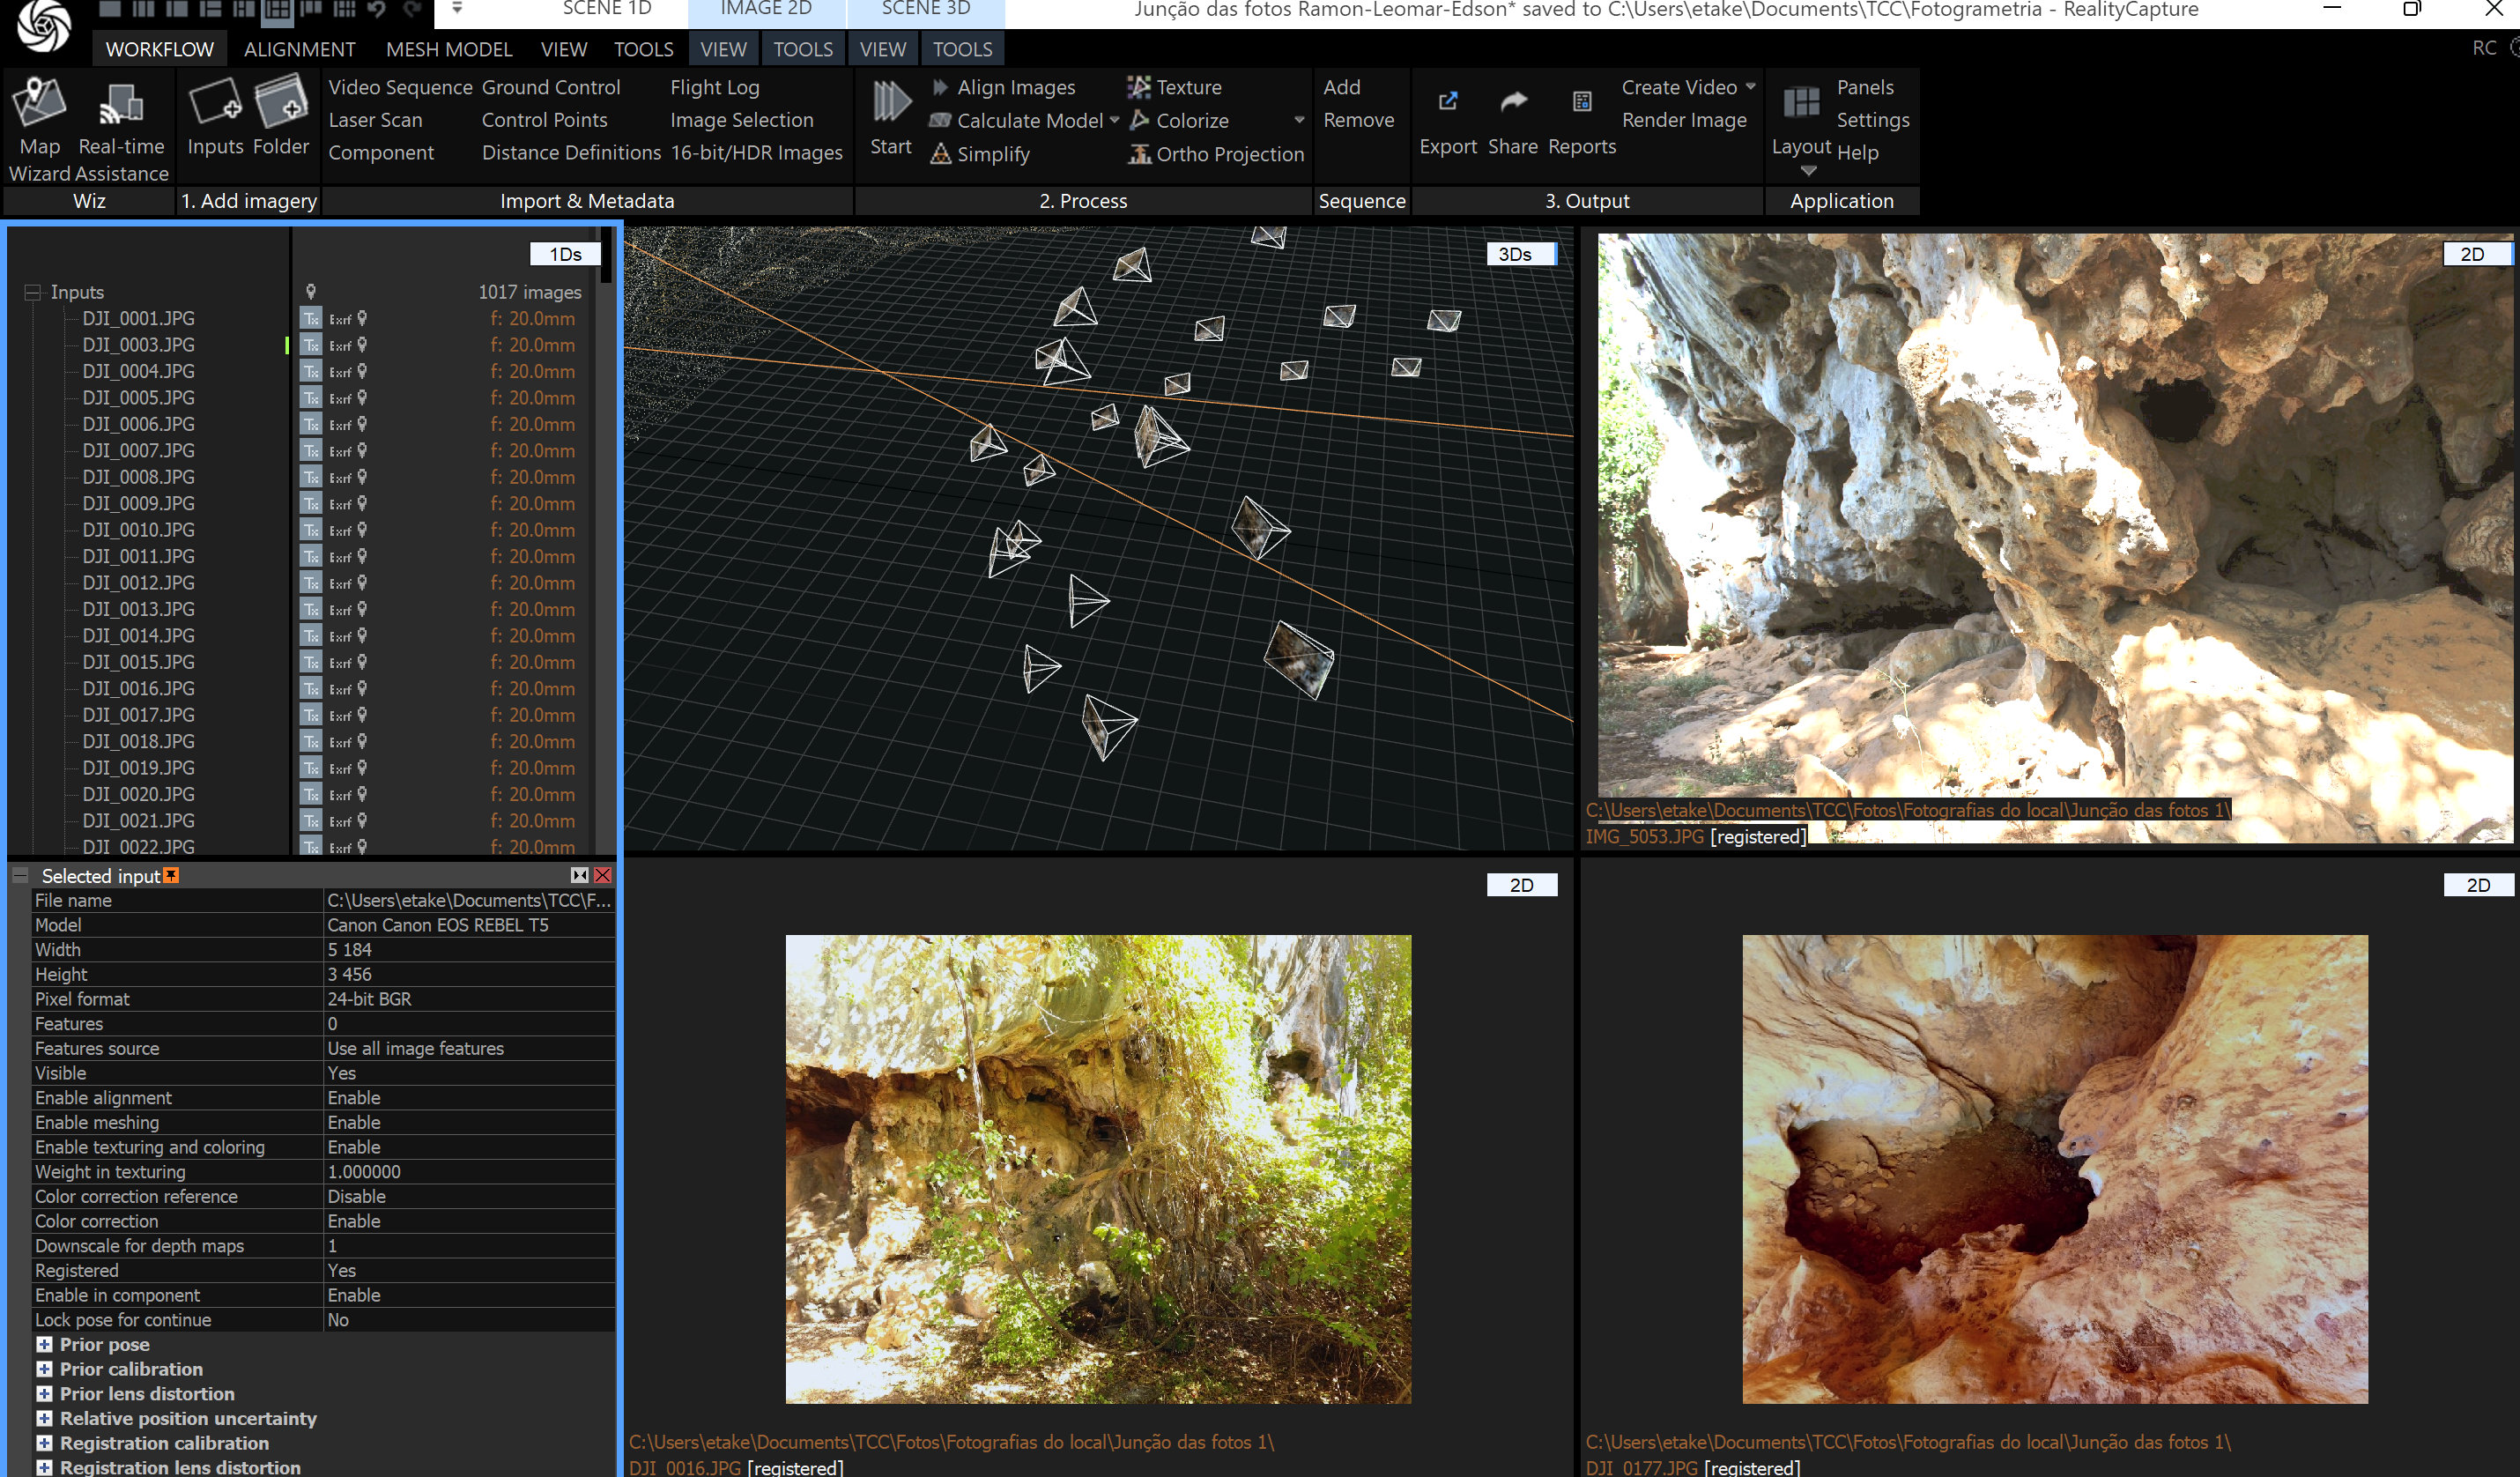
\includegraphics[height=8cm, keepaspectratio]{img/reality e fotogrametria processo/cameras alinhamento.png}
        \caption{Alinhamento das imagens pelo software Reality Capture. \\
            \textbf{Fonte:} Elaborado pelo autor, 2025.}
        \label{fig:alinhamento}
\end{figure}

\begin{figure}[H]
        \centering
        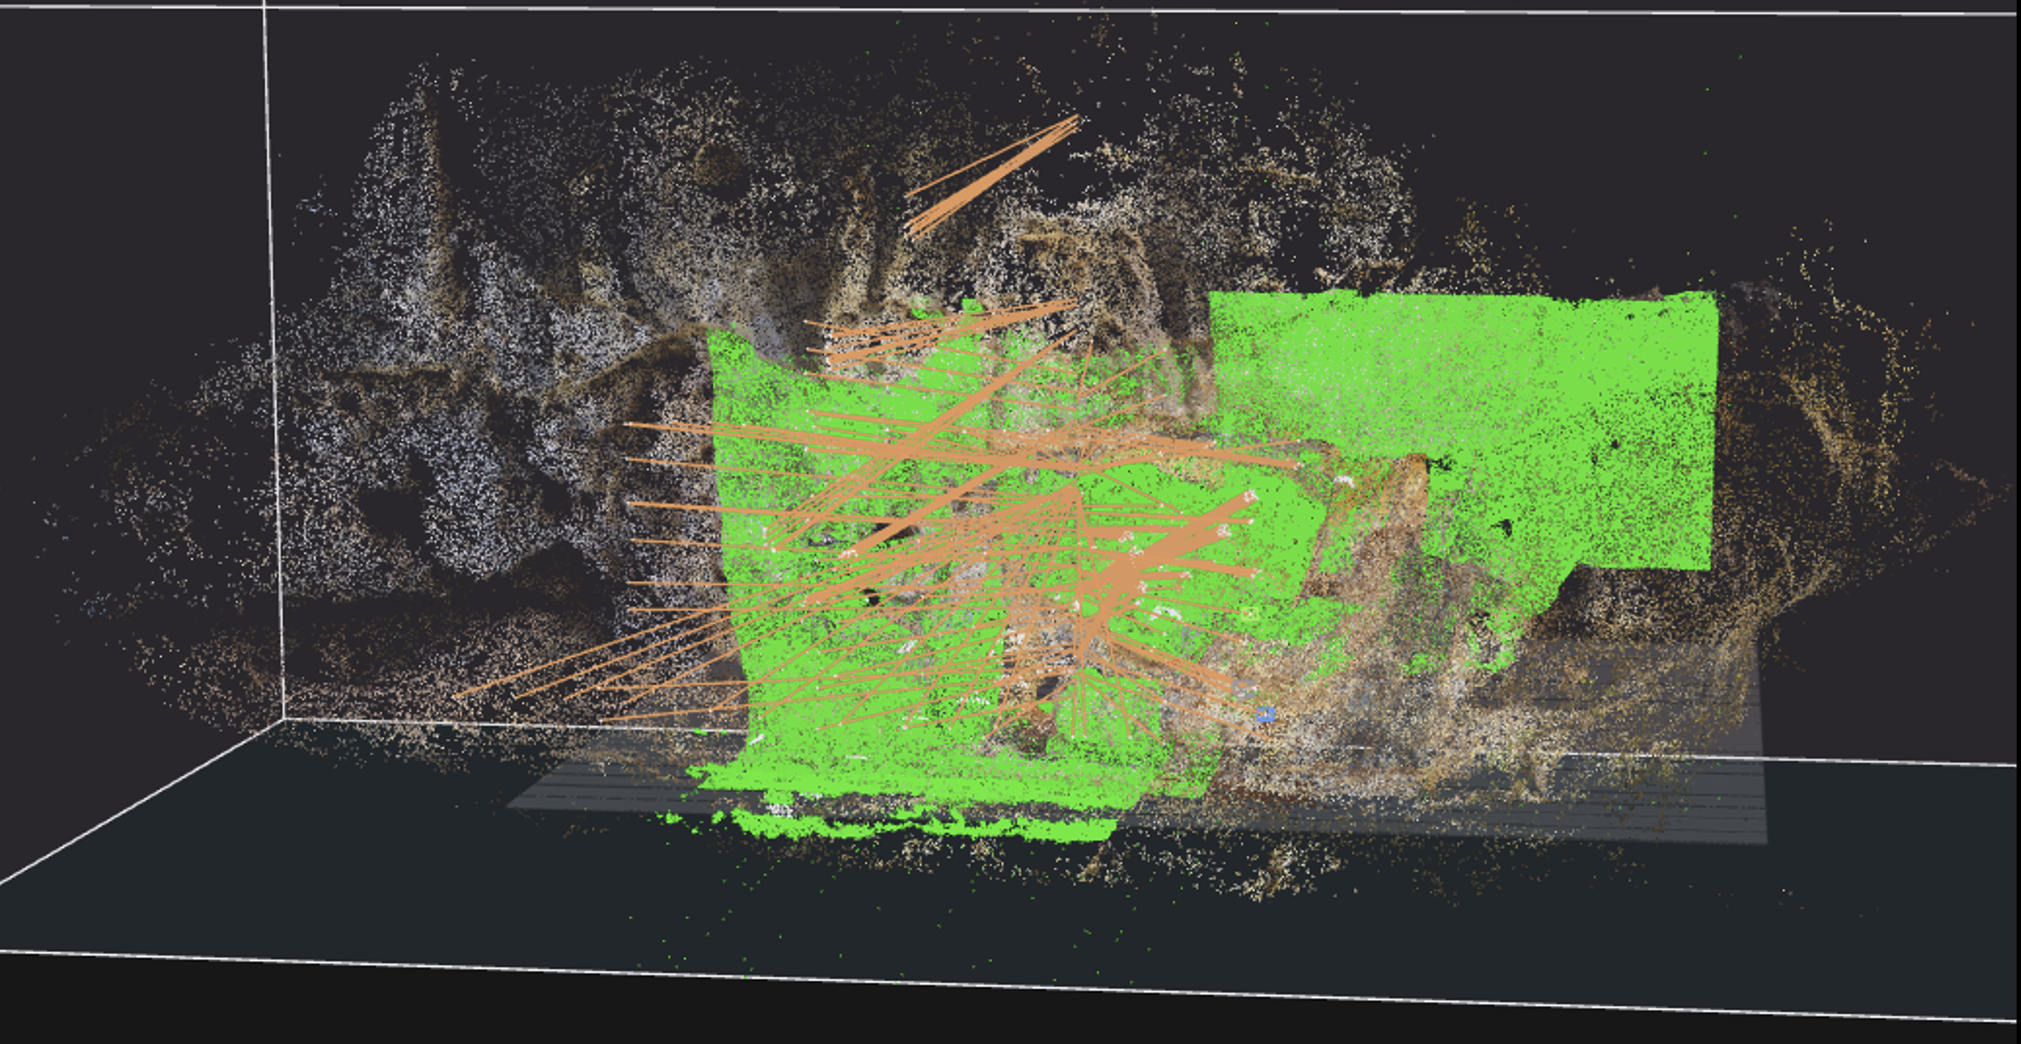
\includegraphics[height=8cm, keepaspectratio]{img/reality e fotogrametria processo/primeiro modelo componente.png}
        \caption{Nuvem de pontos densa. \\
            \textbf{Fonte:} Elaborado pelo autor, 2025.}
        \label{fig:nuvem de pontos}
\end{figure}


\item \textbf{Filtragem e Recorte} \\
Para eliminar pontos indesejados, como vegetação ou objetos móveis, foi realizada uma filtragem manual iterativa. Esta etapa é essencial para garantir que apenas os elementos relevantes sejam incluídos no modelo final.
\begin{figure}[H]
        \centering
        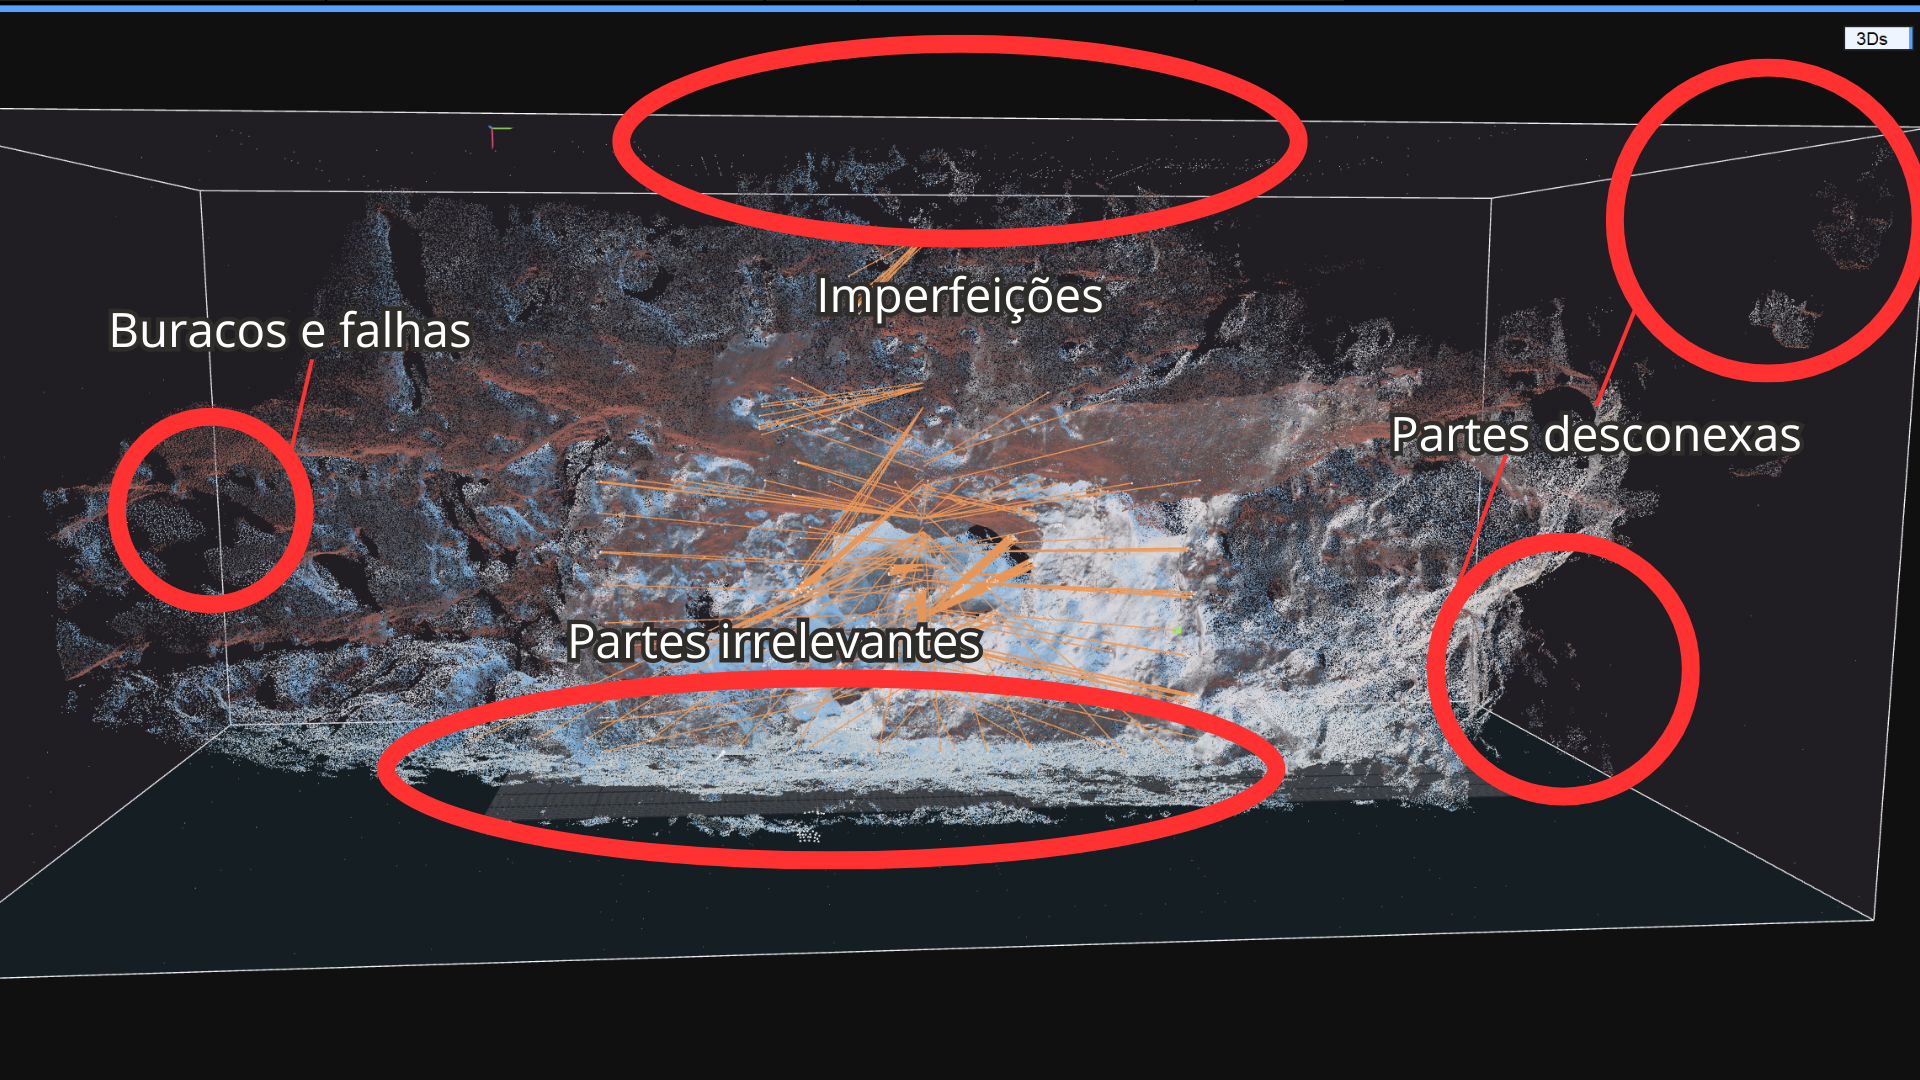
\includegraphics[height=8cm, keepaspectratio]{img/reality e fotogrametria processo/Criação de nuvem de pontos.png}
        \caption{Identificação dos pontos indesejados para filtragem. \\
            \textbf{Fonte:} Elaborado pelo autor, 2025.}
        \label{fig:filtragem}
\end{figure}

\item \textbf{Criação do Modelo 3D} \\
Com base na nuvem de pontos densa filtrada, o software gerou a malha poligonal do modelo 3D, como mostra a Figura \ref{fig:modelo 3D solido}. O modelo inicial continha 102 milhões de polígonos, resultando em um nível de detalhe extremamente alto, mas também em um arquivo muito pesado.
\begin{figure}[H]
        \centering
        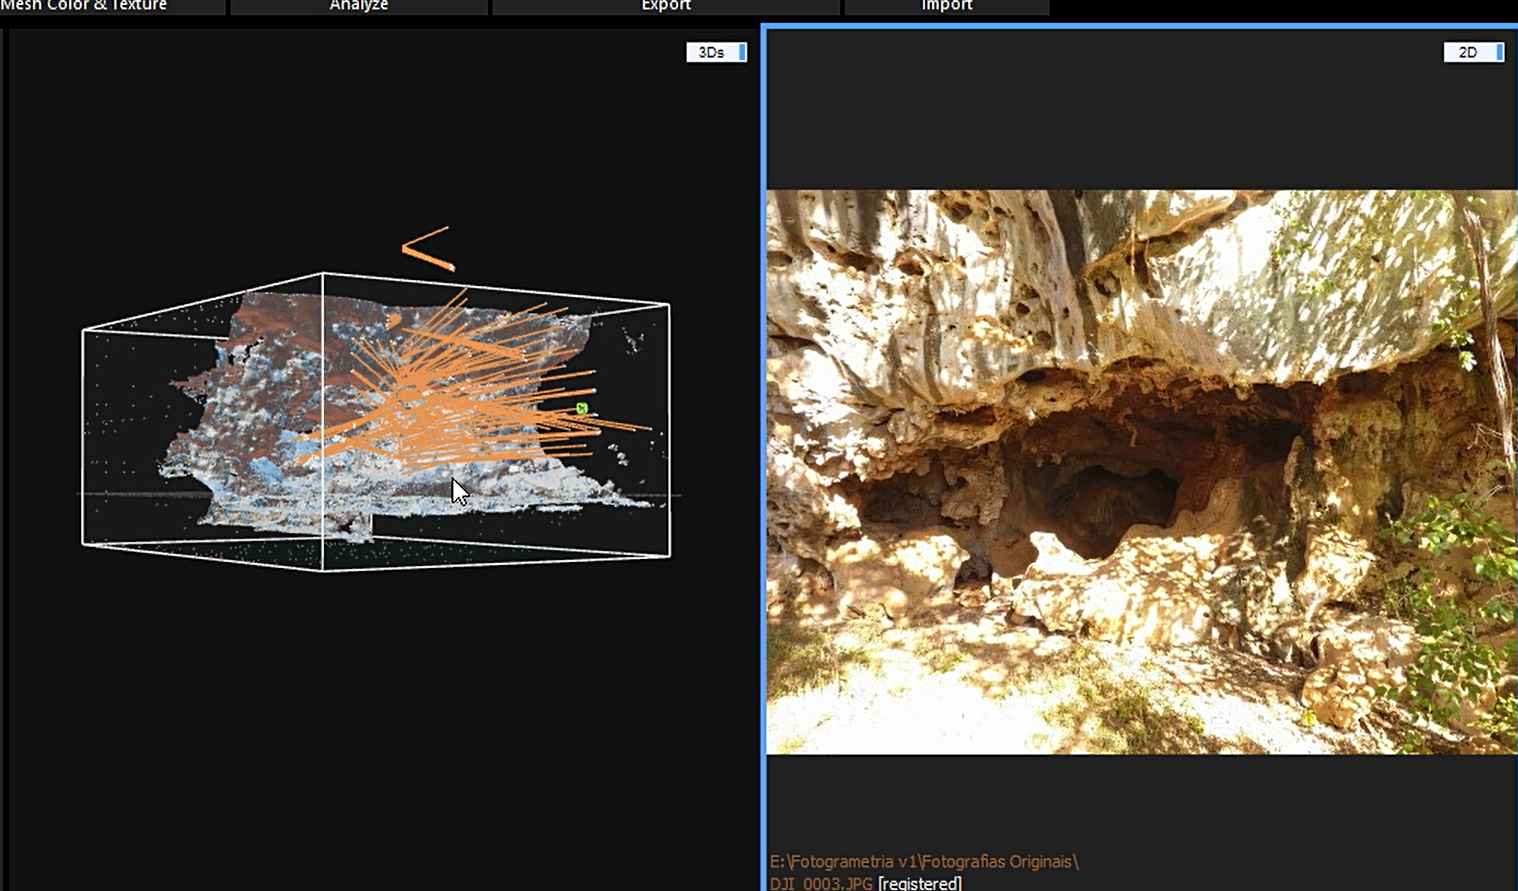
\includegraphics[height=8cm, keepaspectratio]{img/reality e fotogrametria processo/modelo solido e foto.png}
        \caption{Identificação dos pontos indesejados para filtragem. \\
            \textbf{Fonte:} Elaborado pelo autor, 2025.}
        \label{fig:modelo 3D solido}
\end{figure}

\item \textbf{Texturização} \\
O processo de texturização atribuiu cores e detalhes visuais à malha poligonal, utilizando informações das imagens originais. A textura gerada foi de alta qualidade, refletindo fielmente as características do ambiente capturado (Figura \ref{fig:texturizado}). Com esse modelo as figuras pré-históricas no interior da gruta ficaram nítidas e altamente visíveis, como mostra a Figura \ref{fig:interior}.

\begin{figure}[H]
        \centering
        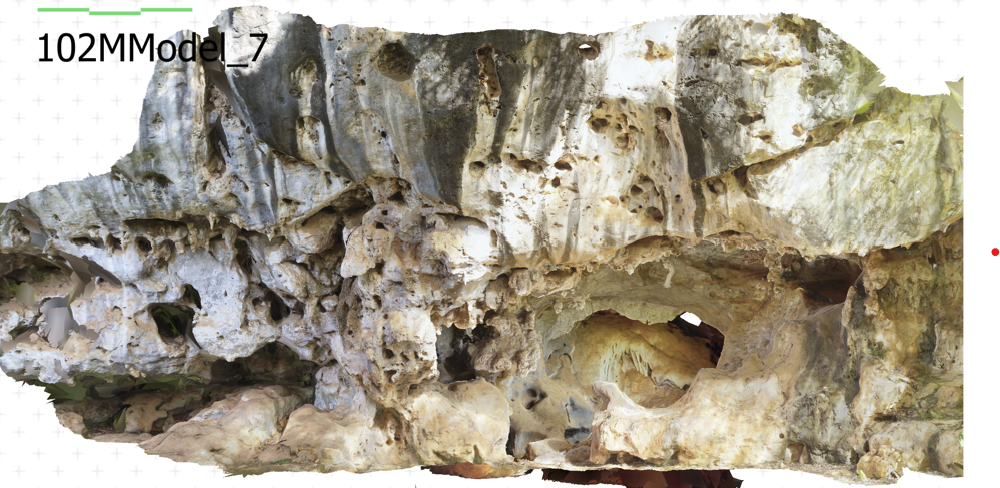
\includegraphics[height=8cm, keepaspectratio]{img/reality e fotogrametria processo/102M textura.png}
        \caption{Modelo texturizado de alta qualidade com 102 milhões de polígonos, parte exterior. \\
            \textbf{Fonte:} Elaborado pelo autor, 2025.}
        \label{fig:texturizado}
\end{figure}
\begin{figure}[H]
        \centering
        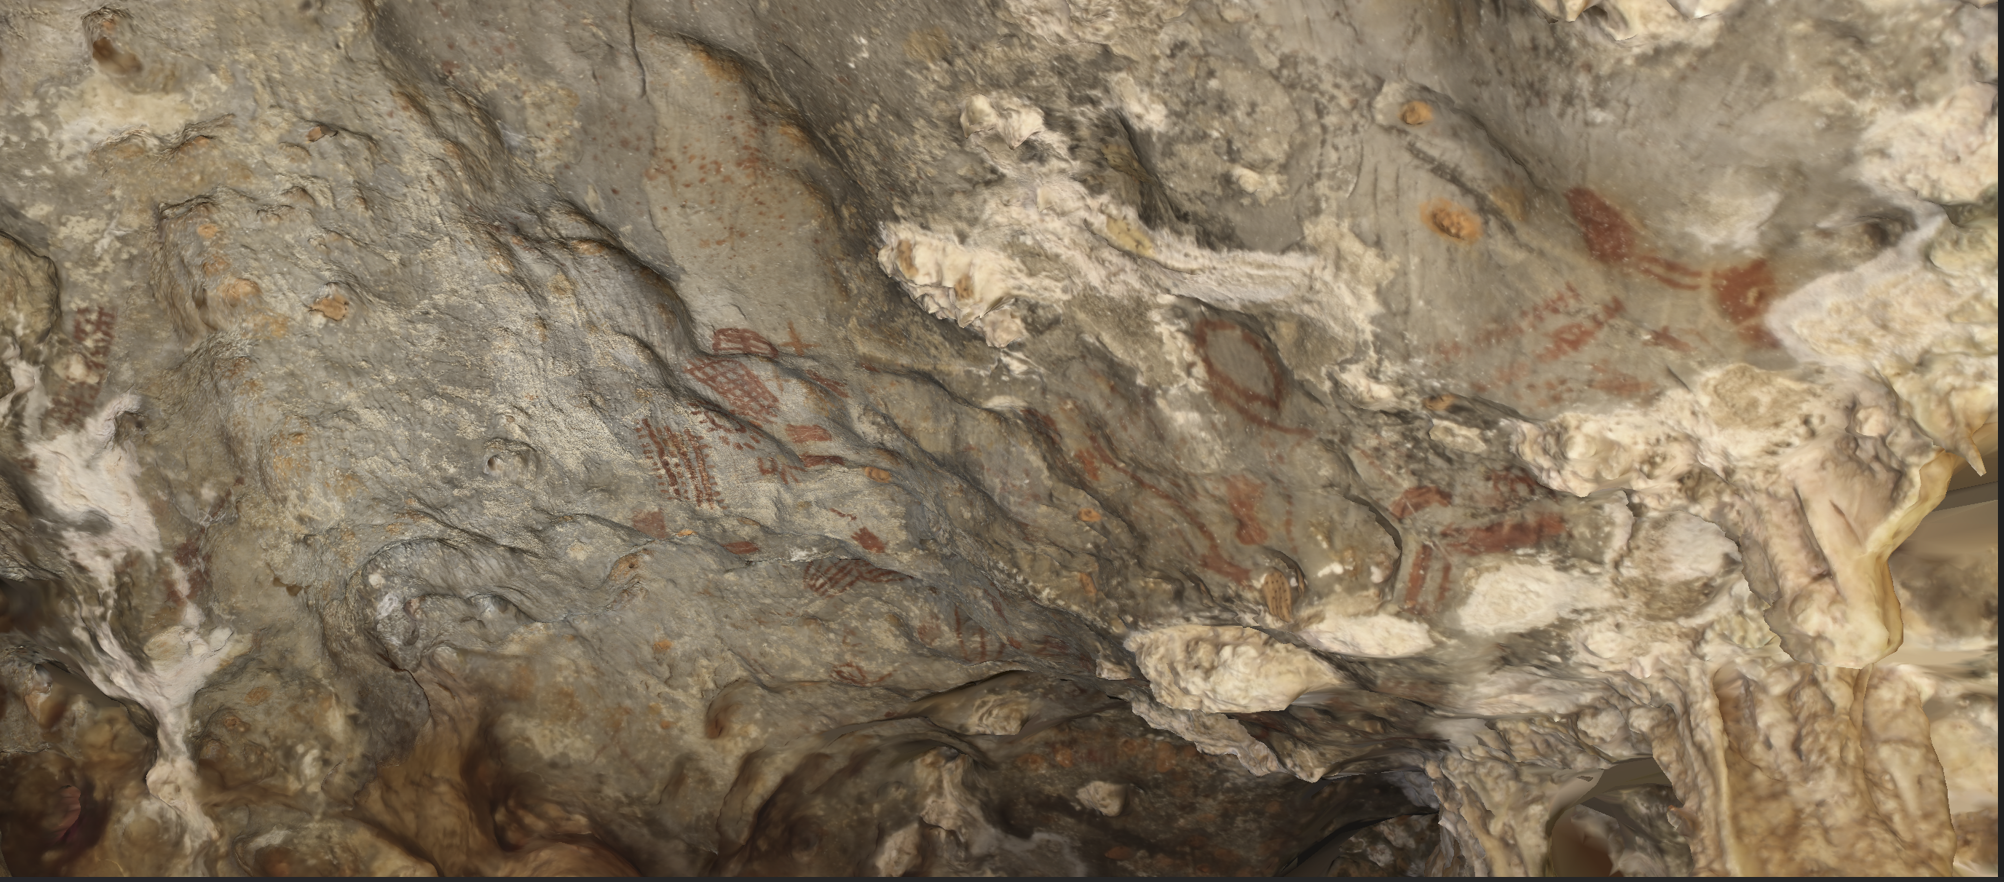
\includegraphics[height=8cm, keepaspectratio]{img/reality e fotogrametria processo/interior.png}
        \caption{Modelo texturizado de alta qualidade com 102 milhões de polígonos, parte interior. \\
            \textbf{Fonte:} Elaborado pelo autor, 2025.}
        \label{fig:interior}
\end{figure}
\end{enumerate}
    \subsection{Simplificação do Modelo 3D, garantindo compatibilidade com a Unreal Engine (RFA001).}
  
Devido ao tamanho do modelo inicial (102 milhões de polígonos), foi necessário realizar um processo de simplificação para torná-lo mais leve e compatível para uso em softwares como a Unreal Engine, que suporta bem até 5 milhões de polígonos. A malha foi reduzida consideravelmente tornando-o mais leve, porém a qualidade ficou muito ruim deixando os desenhos praticamente apagados, como mostra a Figura \ref{fig:modelo ruim}

\begin{figure}[H]
    \centering
    % Primeira figura
    \begin{minipage}{0.45\textwidth} % Reduzi a largura para 45%
        \centering
        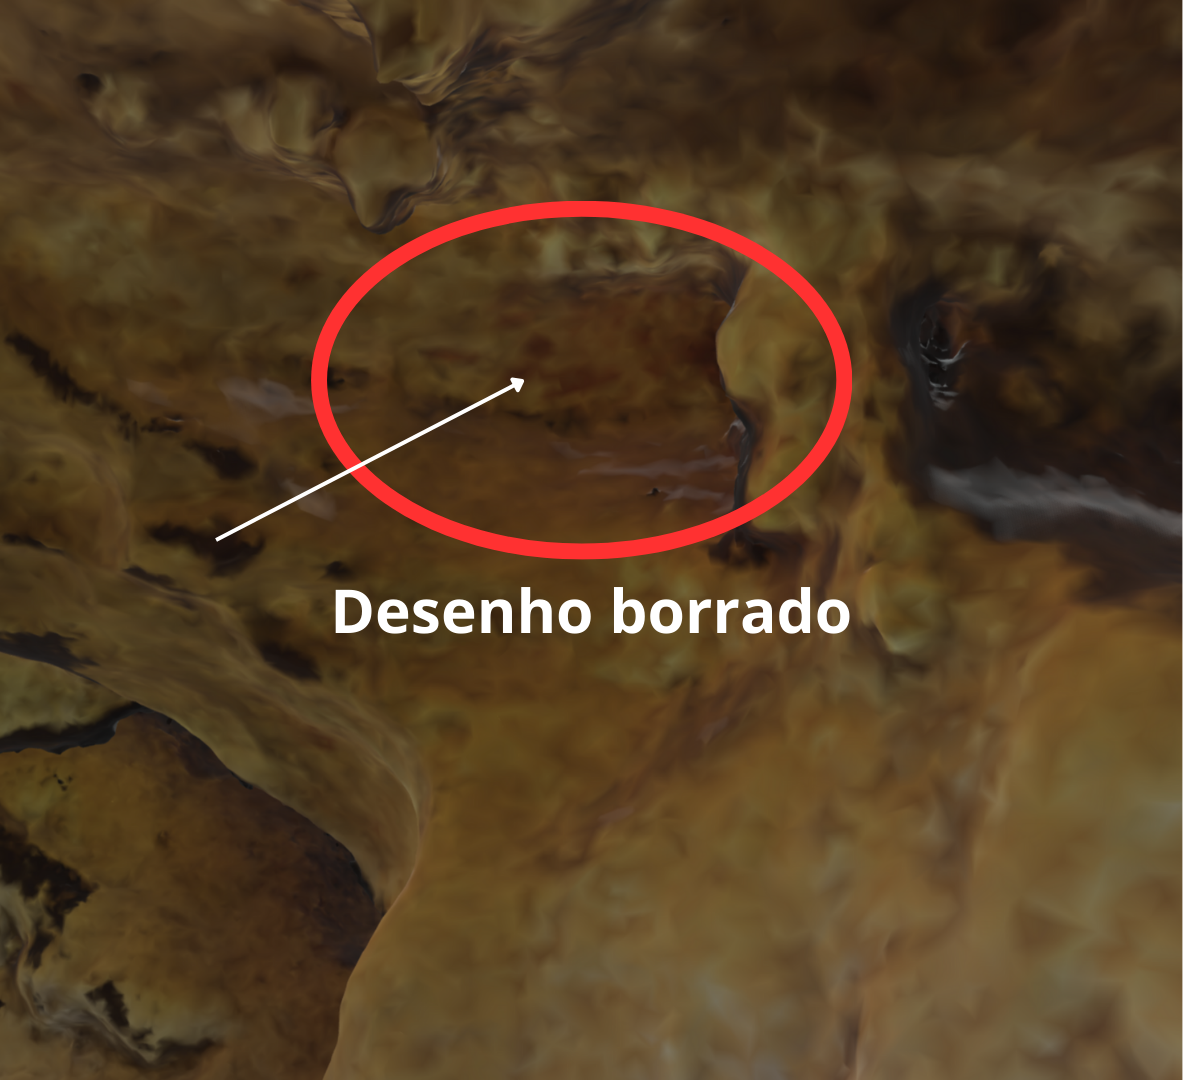
\includegraphics[height=5cm, keepaspectratio]{img/reality e fotogrametria processo/modelo ruim.png}
        \caption{Modelo simplificado com 5 milhões \\ de polígonos. Desenho apagado. \\
            \textbf{Fonte:} Elaborado pelo autor, 2025.}
        \label{fig:modelo ruim}
    \end{minipage}
    \hspace{1cm} % Espaço fixo de 0.5cm entre as figuras
    % Segunda figura
    \begin{minipage}{0.45\textwidth} % Reduzi a largura para 45%
        \centering
        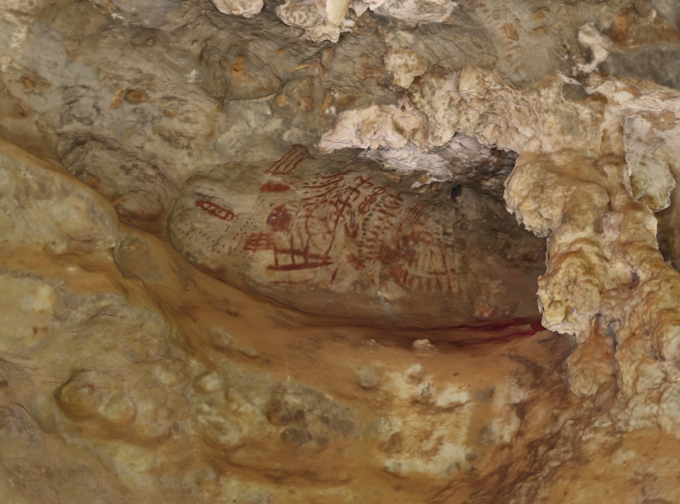
\includegraphics[height=5cm, keepaspectratio]{img/reality e fotogrametria processo/desenho bom retroprojeção.png}
        \caption{Modelo simplificado com reprojeção \\ de textura. \\
            \textbf{Fonte:} Elaborado pelo autor, 2025.}
        \label{fig:desenho bom}
    \end{minipage}
\end{figure}

  \subsection{Reprojeção de textura do modelo de alta resolução para o modelo simplificado, mantendo a qualidade visual.} 
  
Para manter a qualidade visual do modelo simplificado, foi aplicada a técnica de reprojeção de textura \ref{fig:desenho bom}. Essa técnica permite utilizar a textura do modelo original de alta qualidade no modelo simplificado, resultando em um equilíbrio ideal entre detalhamento visual e peso computacional. Primeiro é feito o processo de \textit{ uv unwrap}, que pode ser traduzido como "desdobramento UV" ou "mapeamento UV" (Figura \ref{fig:unwrap}). Esta etapa minimiza distorções e sobreposições, garantindo que a textura se encaixe ao objeto 3D de forma realística, facilitando a transposição de texturas de um modelo para o outro. 
\begin{figure}[H]
        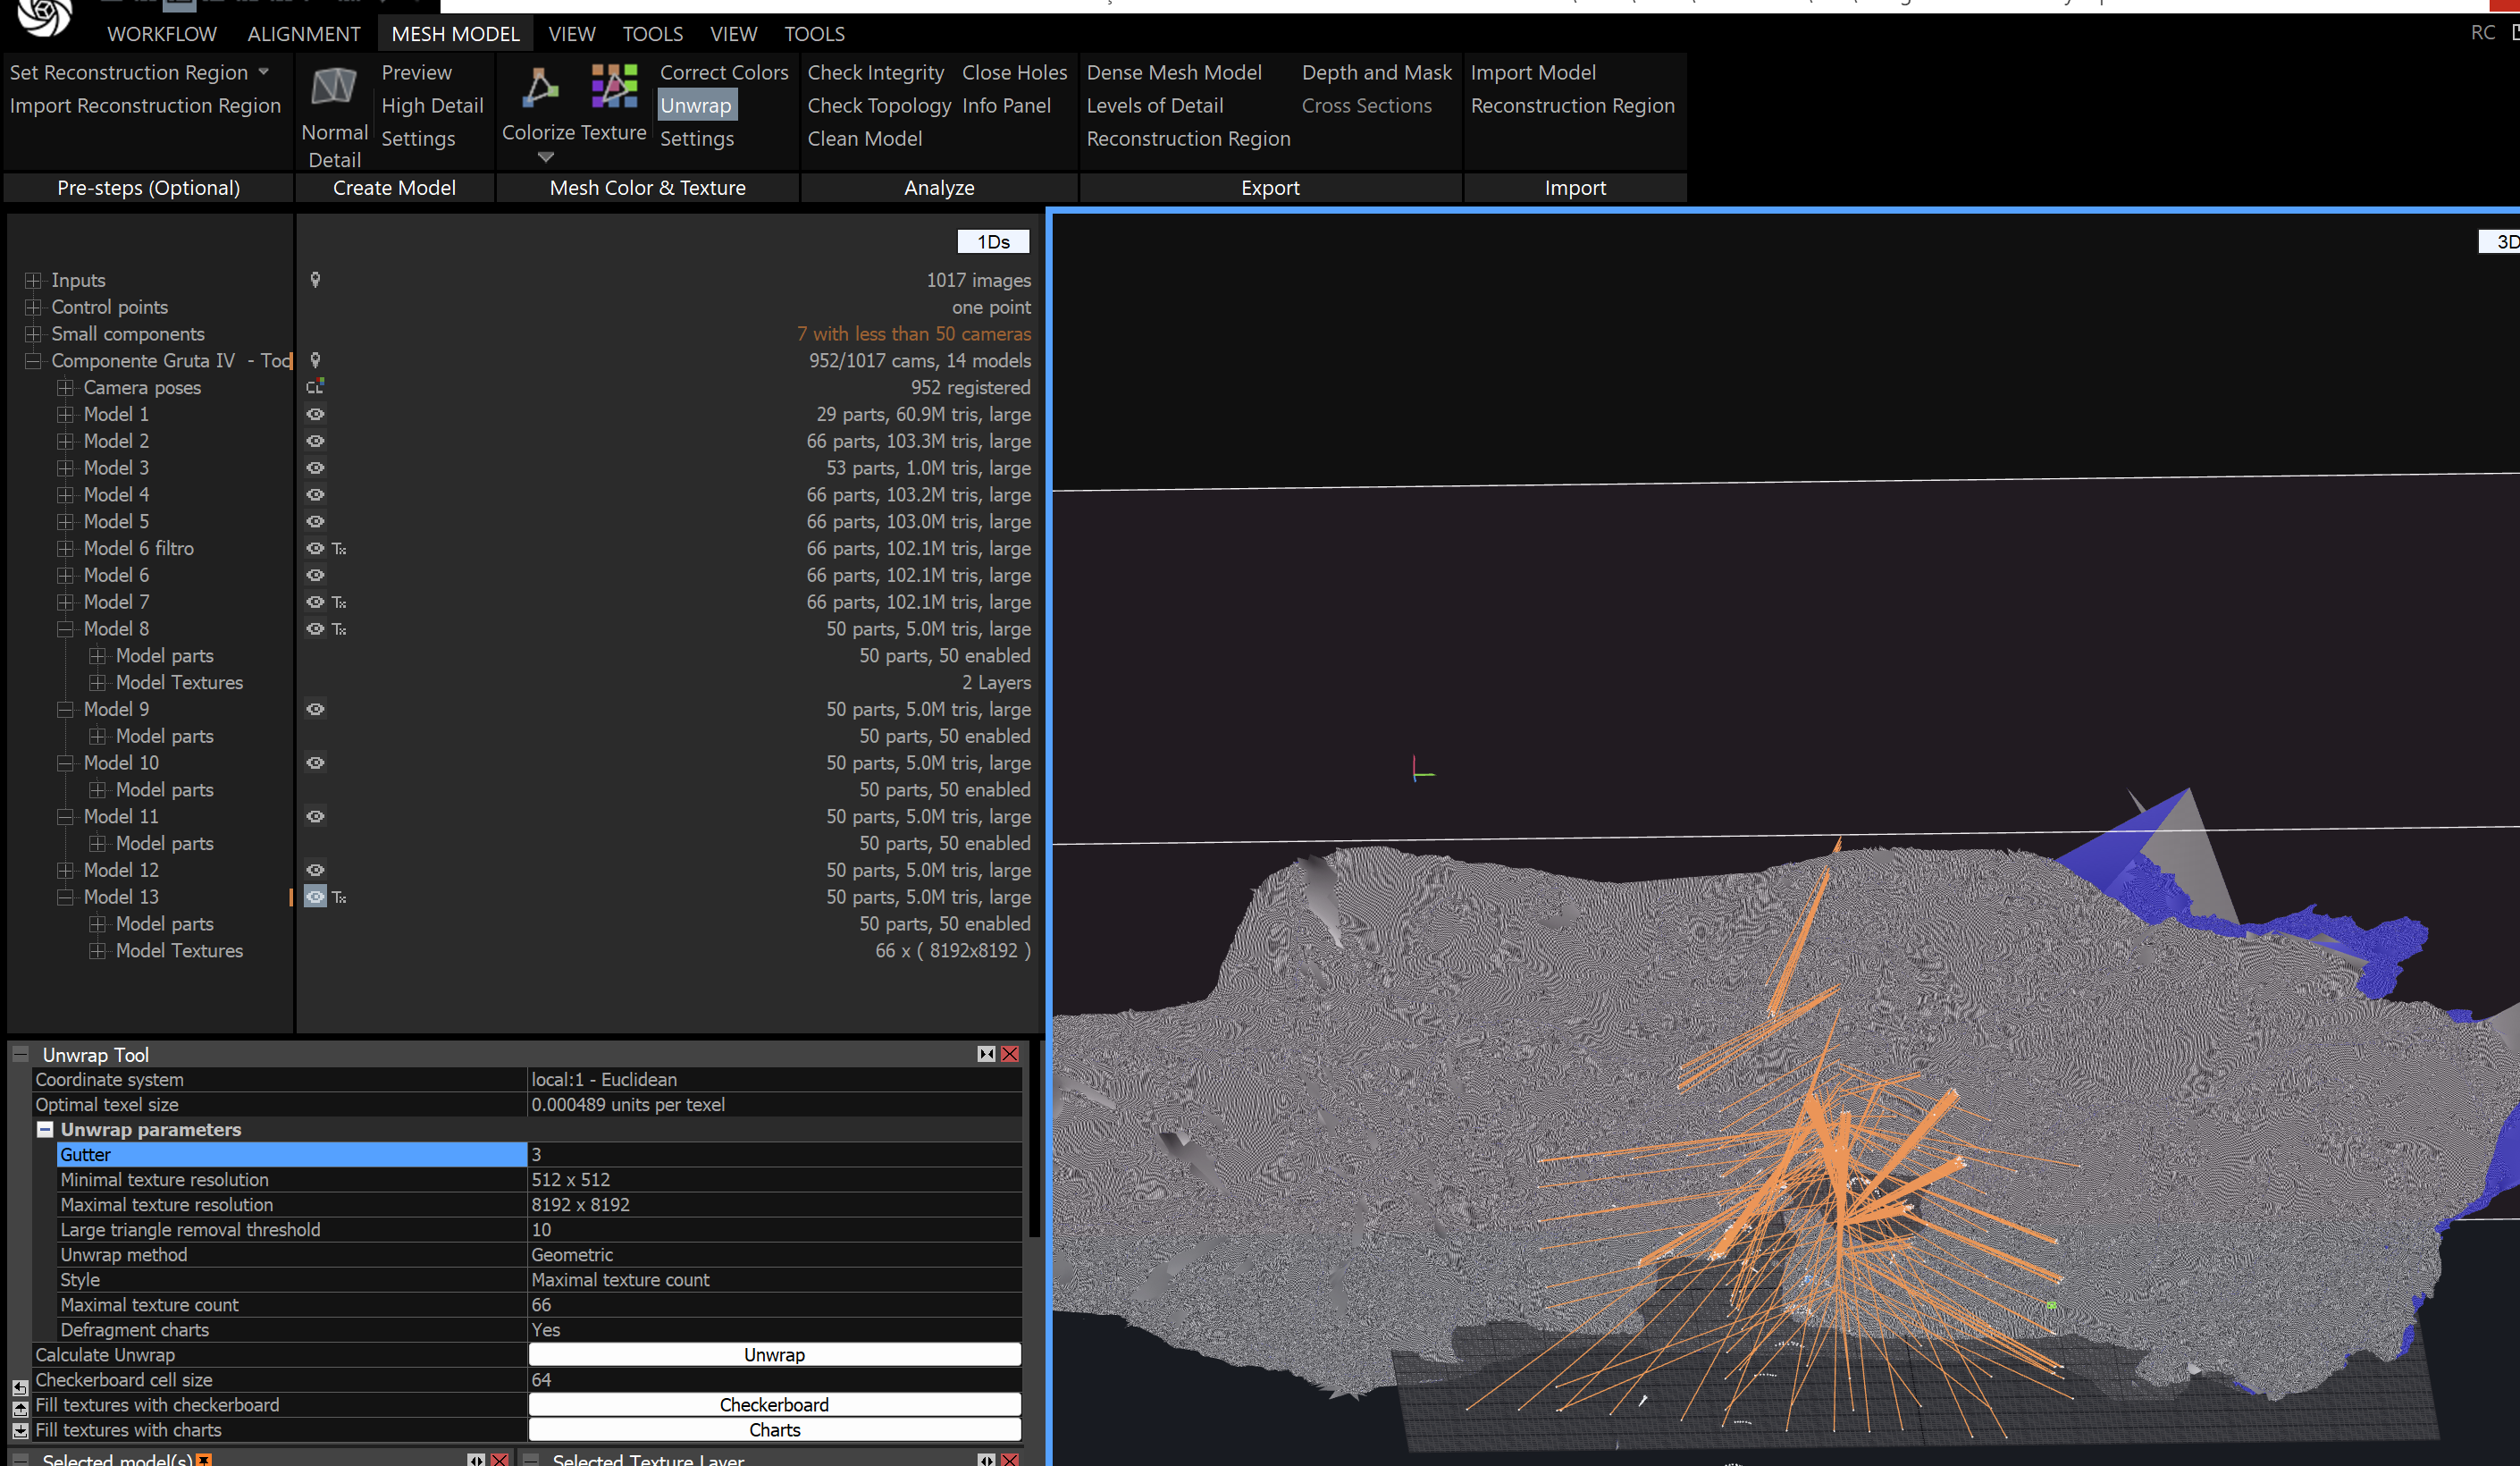
\includegraphics[height=8cm, keepaspectratio]{img/reality e fotogrametria processo/unwrap.png}
        \caption{Processo de Mapeamento UV. \\
            \textbf{Fonte:} Elaborado pelo autor, 2025.}
        \label{fig:unwrap}
\end{figure}

Todo o processo no Reality Capture é demorado e cada etapa pode consumir várias horas. Um dos processos mais rápidos foi o de reprojeção de textura que demorou cerca de apenas 2 horas utilizando um Galaxybook 4 ultra com 32 Gigas de memória RAM, placa de Vídeo NVIDIA 4070 e processador Intel(R) Core(TM) Ultra 9 185H   2.50 GHz com 22 núcleos. Na Figura \ref{fig:reprojecao tempo} pode ser vista uma captura de tela do software processando a reprojeção.
\begin{figure}[H]
        \centering
        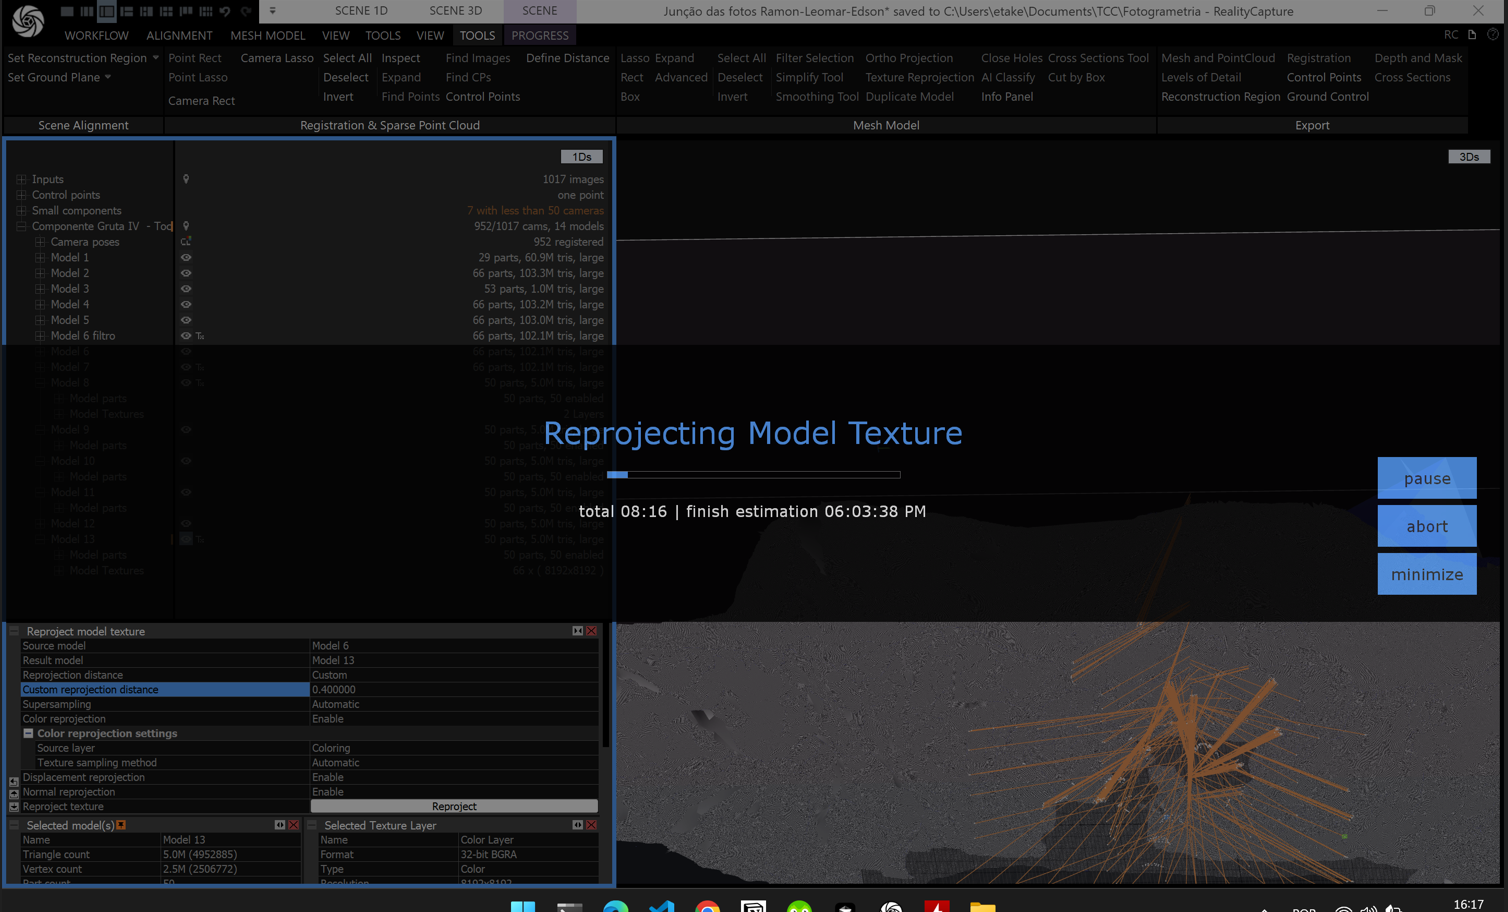
\includegraphics[height=8cm, keepaspectratio]{img/reality e fotogrametria processo/reprojeção.png}
        \caption{Processamento da reprojeção de textura. \\
            \textbf{Fonte:} Elaborado pelo autor, 2025.}
        \label{fig:reprojecao tempo}
\end{figure}


\end{enumerate}
\subsection*{Considerações Finais do Ciclo 1}
O processo de fotogrametria no Reality Capture demonstrou ser uma ferramenta poderosa para a geração de modelos 3D detalhados. A combinação de técnicas como a simplificação de malhas e a reprojeção de textura permitiu criar modelos otimizados para uso em softwares como a Unreal Engine, mantendo alta qualidade visual. Este fluxo de trabalho é essencial para aplicações em um ambiente virtual, a qual é a próxima etapa.


% Ciclo 2
\section{Ciclo 2: Construção do Ambiente Virtual na Unreal Engine}
\label{sec:ciclo2_unreal}
\label{sec:ciclo2_unreal}
A escolha da plataforma Unreal Engine 5.4 para a criação do ambiente virtual 3D se justifica pela sua capacidade de gerar experiências imersivas e interativas. O Unreal Engine é um motor de criação de jogos amplamente utilizado na indústria de jogos, cinema e arquitetura. A plataforma oferece recursos como simulação de luz, movimentações de câmera e personagens, e a possibilidade de interagir com os elementos do ambiente, tornando o ambiente virtual 3D mais realista e envolvente \citep{silva2022realidade}.

\textbf{Objetivo do ciclo}: Desenvolver um ambiente virtual interativo na Unreal Engine 5.4 que atenda aos requisitos funcionais RFA002 (Navegação em Terceira Pessoa), RFA003 (Alternância de Câmera), RFA004 (Avatar Personalizado), bem como aos requisitos não funcionais RNFA001 (Compatibilidade com Windows) e RNFA002  (Instalação Simplificada). Este ciclo aborda a importação do modelo 3D otimizado, a criação do cenário virtual, a implementação de funcionalidades interativas e a preparação para distribuição.

\subsection{Importação do Modelo 3D Otimizado na Unreal Engine 5.4}
O modelo 3D simplificado e texturizado, gerado no Reality Capture durante o Ciclo 1, foi importado para a Unreal Engine 5.4. Durante a importação, foram realizados ajustes nas propriedades do modelo, incluindo:
\begin{enumerate}
    \item \textbf{Escala e Posicionamento}: O modelo foi ajustado para corresponder à escala do ambiente virtual, garantindo que as proporções fossem consistentes com os outros elementos do cenário. A Figura \ref{fig:escala} mostra uma foto real de um ser humano como referência de tamanho para o ajuste de proporção do modelo 3D.
    \item \textbf{Otimização de Materiais}: Os materiais do modelo foram ajustados para aproveitar o sistema Nanite da Unreal Engine, que permite renderizar geometrias complexas sem comprometer o desempenho.
    \item \textbf{Colisão}: Foram configuradas colisões automáticas para permitir interações realistas entre o avatar e o ambiente. Em áreas específicas, como entradas e interior da gruta, foram criadas colisões personalizadas para garantir precisão. Como mostrado na Figura \ref{fig:colisao}
\end{enumerate}
% A Figura \ref{fig:modelo_importado} ilustra o modelo 3D após a importação e ajustes iniciais.

\begin{figure}[H]
        \centering
        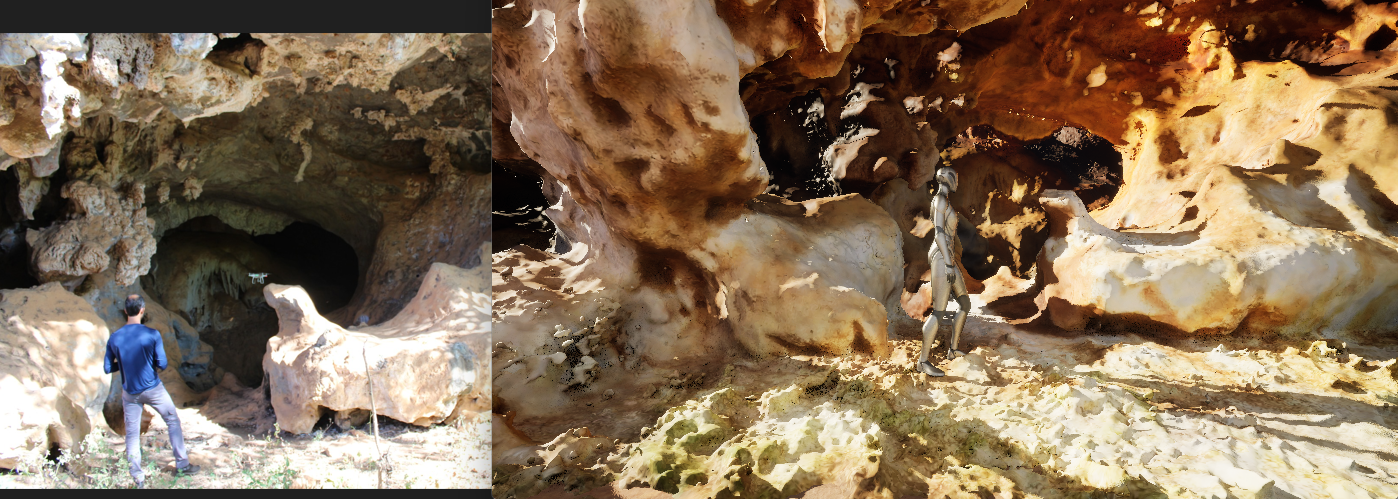
\includegraphics[height=6cm, keepaspectratio]{img/unreal/escala.png}
        \caption{Ajuste na escala comparando com uma foto real de\\ um ser humano na entrada da gruta. \\
            \textbf{Fonte:} Elaborado pelo autor, 2025.}
        \label{fig:escala}
\end{figure}

\begin{figure}[H]
        \centering
        \includegraphics[height=8cm, keepaspectratio]{img/unreal/colisão.png}
        \caption{Colisão dos objetos na cena dentro da Unreal Engine. \\
            \textbf{Fonte:} Elaborado pelo autor, 2025.}
        \label{fig:colisao}
\end{figure}


\subsection{Criação do Cenário Virtual}
Para enriquecer o ambiente virtual, foram adicionados elementos complementares ao modelo principal, como vegetação, gramado, pedras e um terreno detalhado. Esses elementos foram criados utilizando \textit{assets} disponíveis no \textit{Marketplace} da \textit{Unreal Engine} e customizados para se integrar harmoniosamente ao modelo 3D da Lapa da Pedra. As principais etapas incluem:
\begin{enumerate}
    \item \textbf{Texturas Realistas}: Foram aplicadas texturas de alta qualidade para criar uma aparência naturalista. A iluminação dinâmica foi configurada para interagir realisticamente com as superfícies, destacando detalhes como sombras e reflexos.
    \item \textbf{Iluminação Dinâmica}: Utilizando o sistema Lumen da Unreal Engine, foi implementada uma iluminação global dinâmica, que simula a interação de luz natural com o ambiente. Isso incluiu a configuração de fontes de luz direcionais para simular o sol e luzes pontuais para áreas internas da gruta.
    \item \textbf{Ambientação Sonora}: Sons ambientes, como vento e pássaros, foram adicionados para aumentar a imersão do usuário no cenário virtual.
\end{enumerate}
A Figura \ref{fig:grama} apresenta o cenário virtual sendo preenchido com elementos de paisagem como árvores, rochas, grama com o modelo 3D integrado ao ambiente.
\begin{figure}[H]
        \centering
        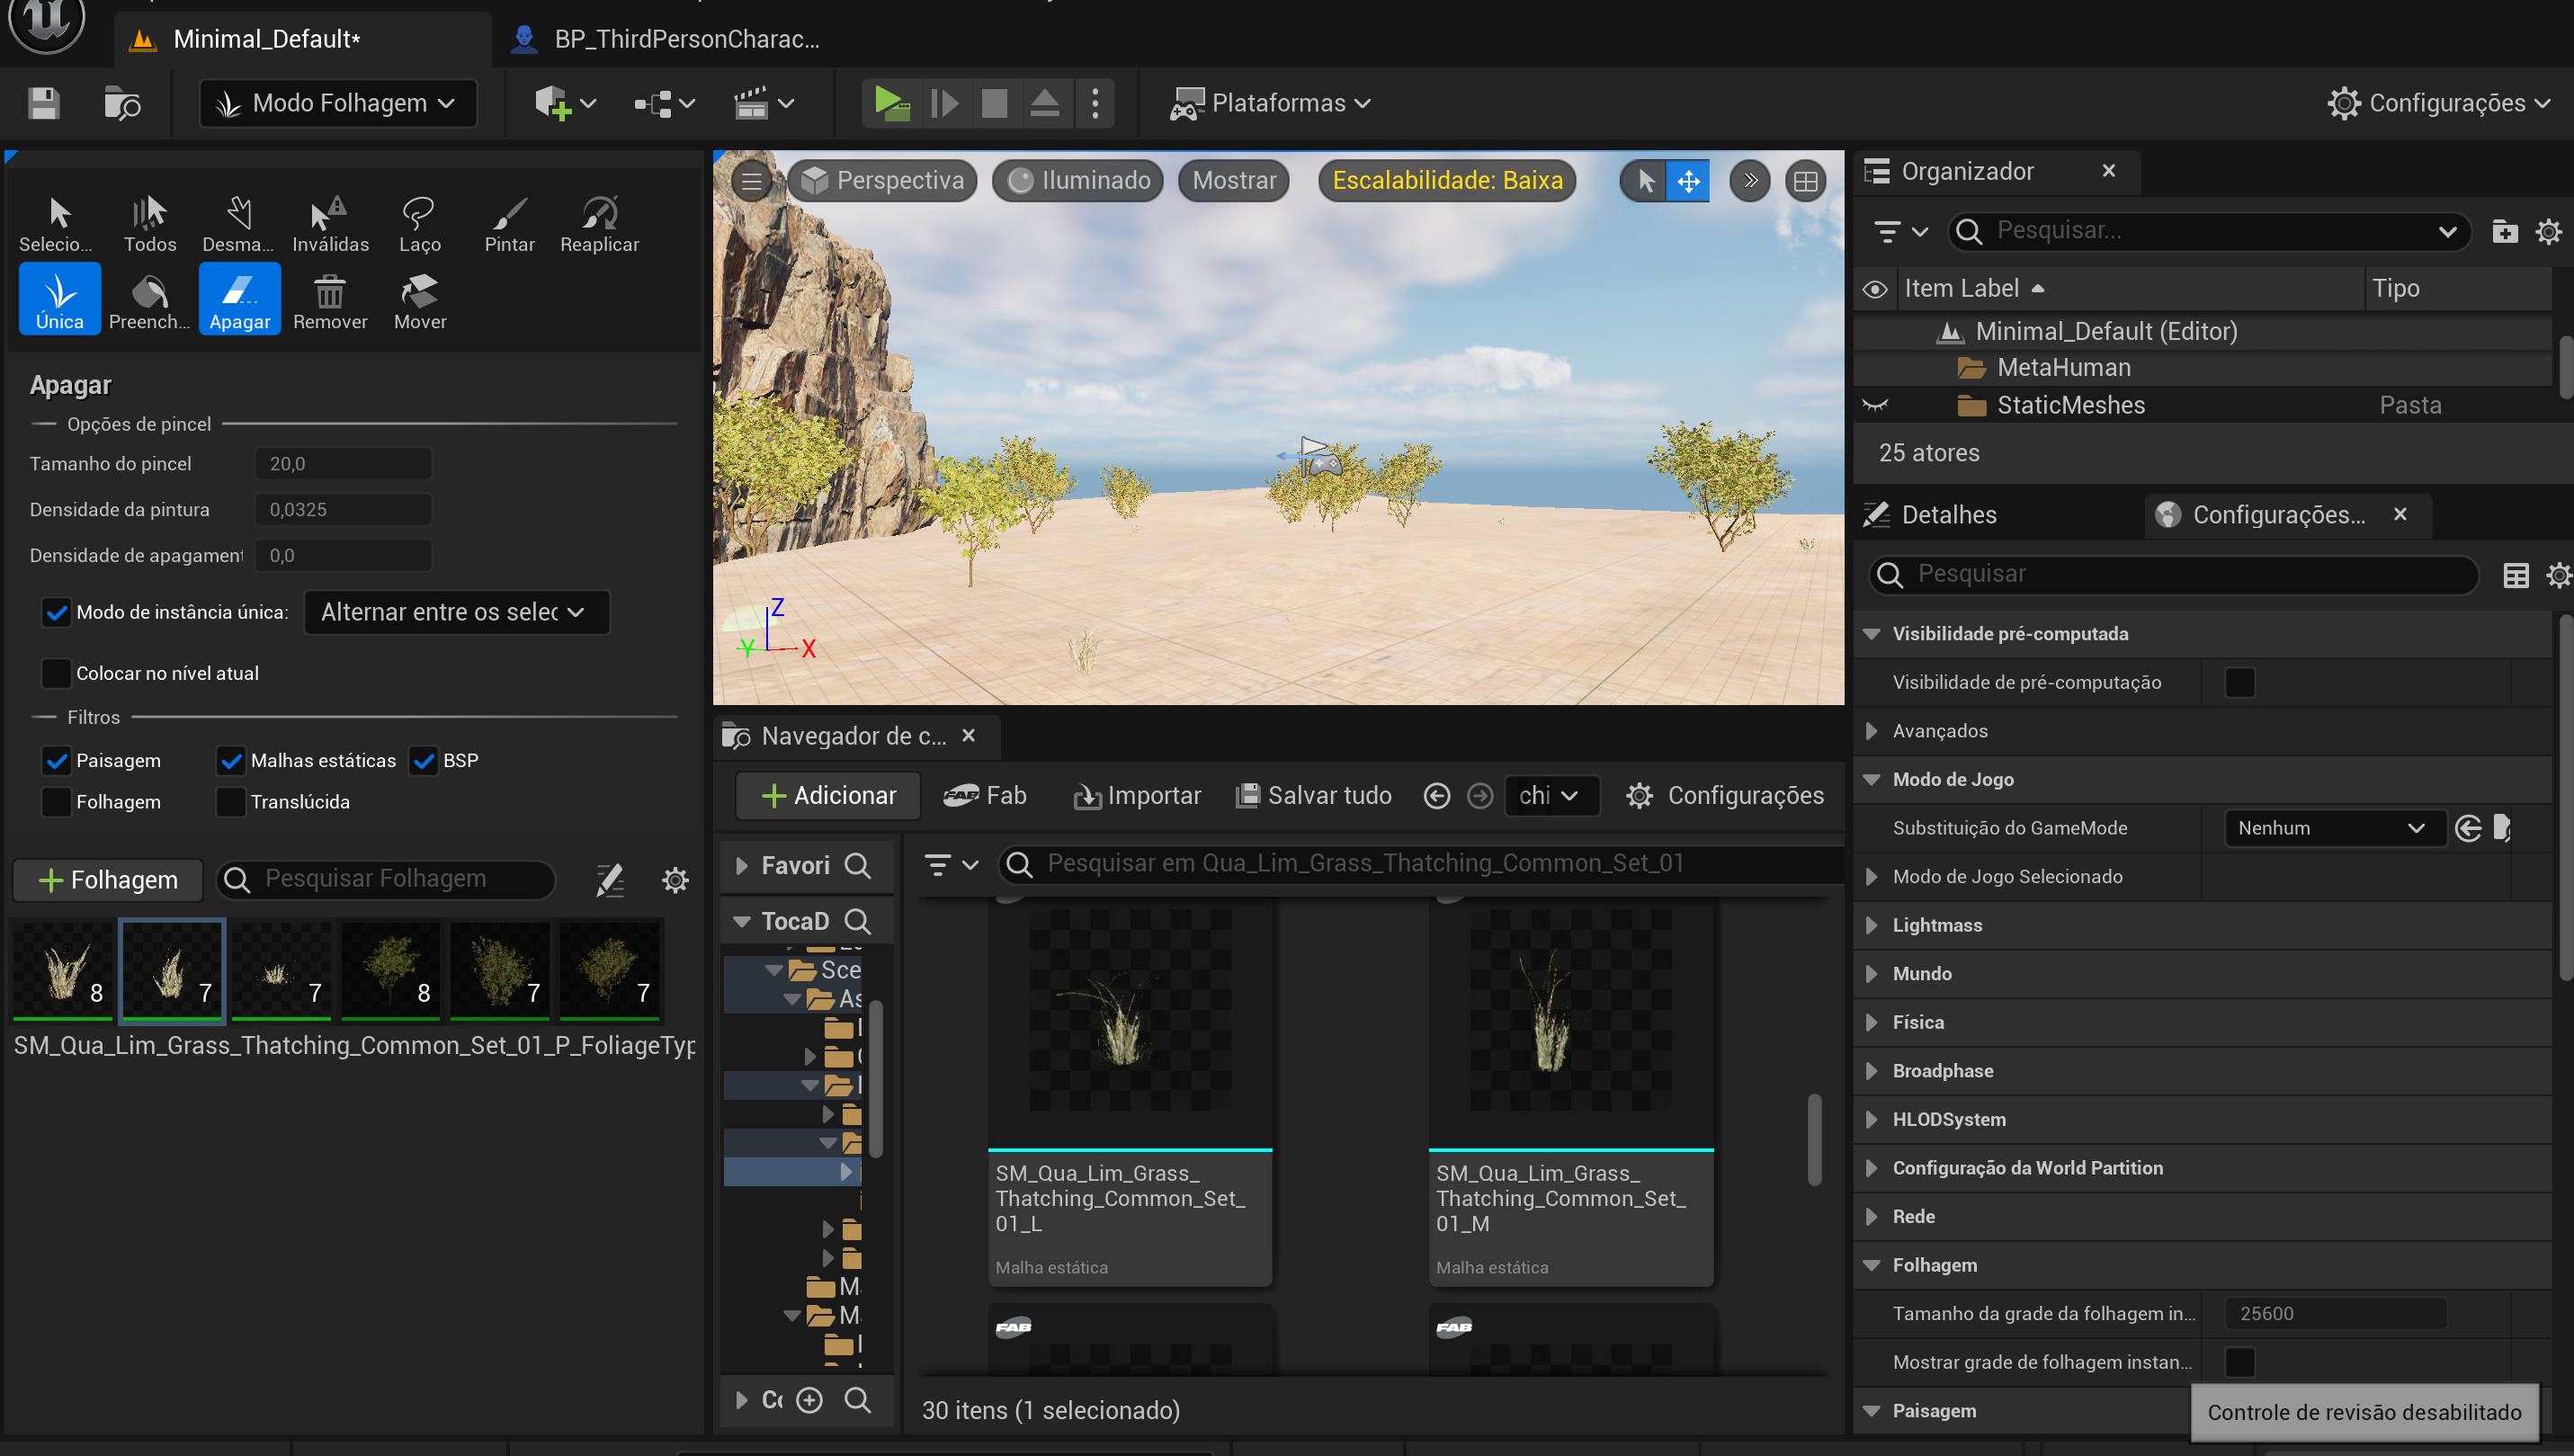
\includegraphics[height=8cm, keepaspectratio]{img/unreal/paisagem grass.png}
        \caption{Processo de criação e preenchimento do cenário. \\
            \textbf{Fonte:} Elaborado pelo autor, 2025.}
        \label{fig:grama}
\end{figure}


\subsection{Implementação do Sistema de Navegação em Terceira Pessoa (RFA002)}
Foi desenvolvido um sistema de navegação em terceira pessoa, permitindo que o usuário controle um avatar interativo e explore o ambiente virtual. Para isso, foi utilizado o Template de Terceira Pessoa fornecido pela Unreal Engine, que foi adaptado para atender às necessidades específicas do projeto. As principais funcionalidades incluem:
\begin{itemize}
    \item Movimentação suave do avatar com controles de teclado e mouse.
    \item Detecção de colisão para evitar que o avatar atravesse paredes ou obstáculos.
\end{itemize}

\subsection{Criação de Avatar Personalizado no Metahuman (RFA004)}
Um avatar personalizado foi criado utilizando o Metahuman Creator, uma ferramenta da Unreal Engine para geração de personagens humanos altamente realistas. O avatar foi projetado para se assemelhar ao professor Edson Borges, com base em referências fotográficas fornecidas. As etapas incluíram a modelagem facial detalhada no Metahuman Creator; a customização barba, roupas e acessórios para refletir a aparência do professor e a importação do avatar para a Unreal Engine e integração com o sistema de controle de personagem (Figura \ref{fig:metahumancamera}).
\end{enumerate}

A Figura \ref{fig:metahumanEdsonn} exibe o avatar finalizado no ambiente virtual.

\begin{figure}[H]
        \centering
\includegraphics[height=8cm, keepaspectratio]{img/unreal/ajuste de câmera edson.png}
        \caption{Importação do Metahuman do professor Edson \\ para se tornar um personagem controlável. \\
            \textbf{Fonte:} Elaborado pelo autor, 2025.}
        \label{fig:metahumancamera}
\end{figure}

\begin{figure}[H]
        \centering
\includegraphics[height=8cm, keepaspectratio]{img/unreal/metahuman dentro da caverna.png}
        \caption{Avatar digital do professor Edson Borges no ambiente virtual. \\
            \textbf{Fonte:} Elaborado pelo autor, 2025.}
        \label{fig:metahumanEdsonn}
\end{figure}


\subsection{Desenvolvimento do Sistema de Alternância de Câmera (RFA003)}
Foi implementado um sistema de alternância de câmera, permitindo que o usuário alterne entre visão em primeira e terceira pessoa. Essa funcionalidade foi desenvolvida utilizando \textit{Blueprints}\footnote{\href{https://dev.epicgames.com/community/learning/tutorials/K8Gx/unreal-engine-comparacao-entre-blueprints-e-c-casos-de-uso}{\textit{Blueprint}} é a linguagem de programação baseada em nós da Unreal Engine. Depois ela é convertida na linguagem de programação C++. }, a linguagem visual de programação da Unreal Engine. O sistema inclui ajustes na posição e orientação das câmeras para garantir uma experiência imersiva e um botão dedicado para alternar entre as câmeras.

A Figura \ref{fig:config_camera} mostra o processo de posicionamento e configuração da câmera. A Figura \ref{fig:alternarcamera} ilustra a alternância de câmera em funcionamento.
Foi configurada a tecla "C"  como sendo responsável por alternar entre as câmeras, e a configuração da \textit{Blueprint} utilizada pode ser vista na Figura \ref{fig:blueprint_camera}.

\begin{figure}[H]
        \centering
        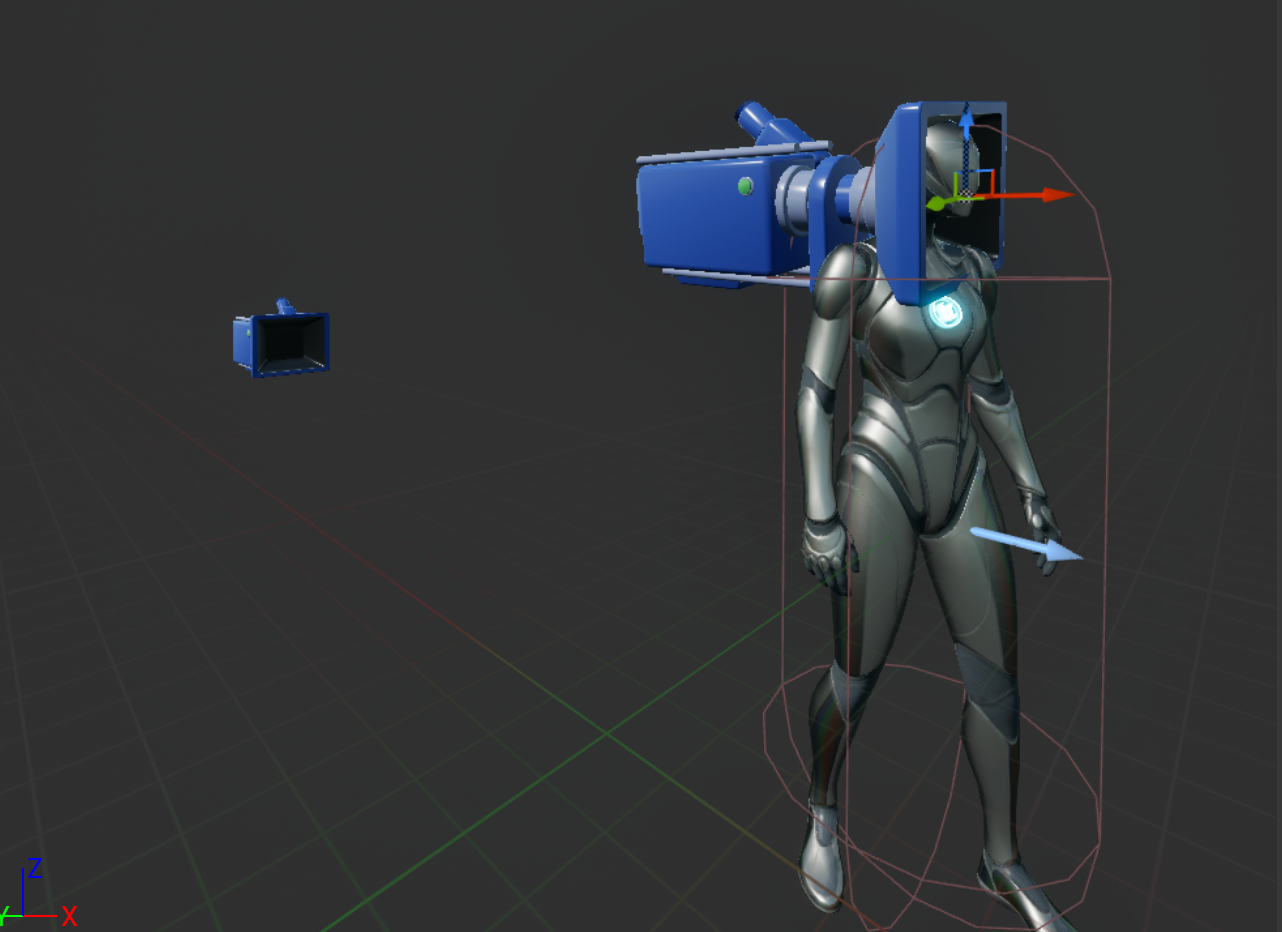
\includegraphics[height=8cm, keepaspectratio]{img/unreal/ajuste de câmera 1ºpessoa.png}
        \caption{Ajuste da câmera para visualização primeira pessoa. \\
            \textbf{Fonte:} Elaborado pelo autor, 2025.}
        \label{fig:config_camera}
\end{figure}

\begin{figure}[H]
        \centering
        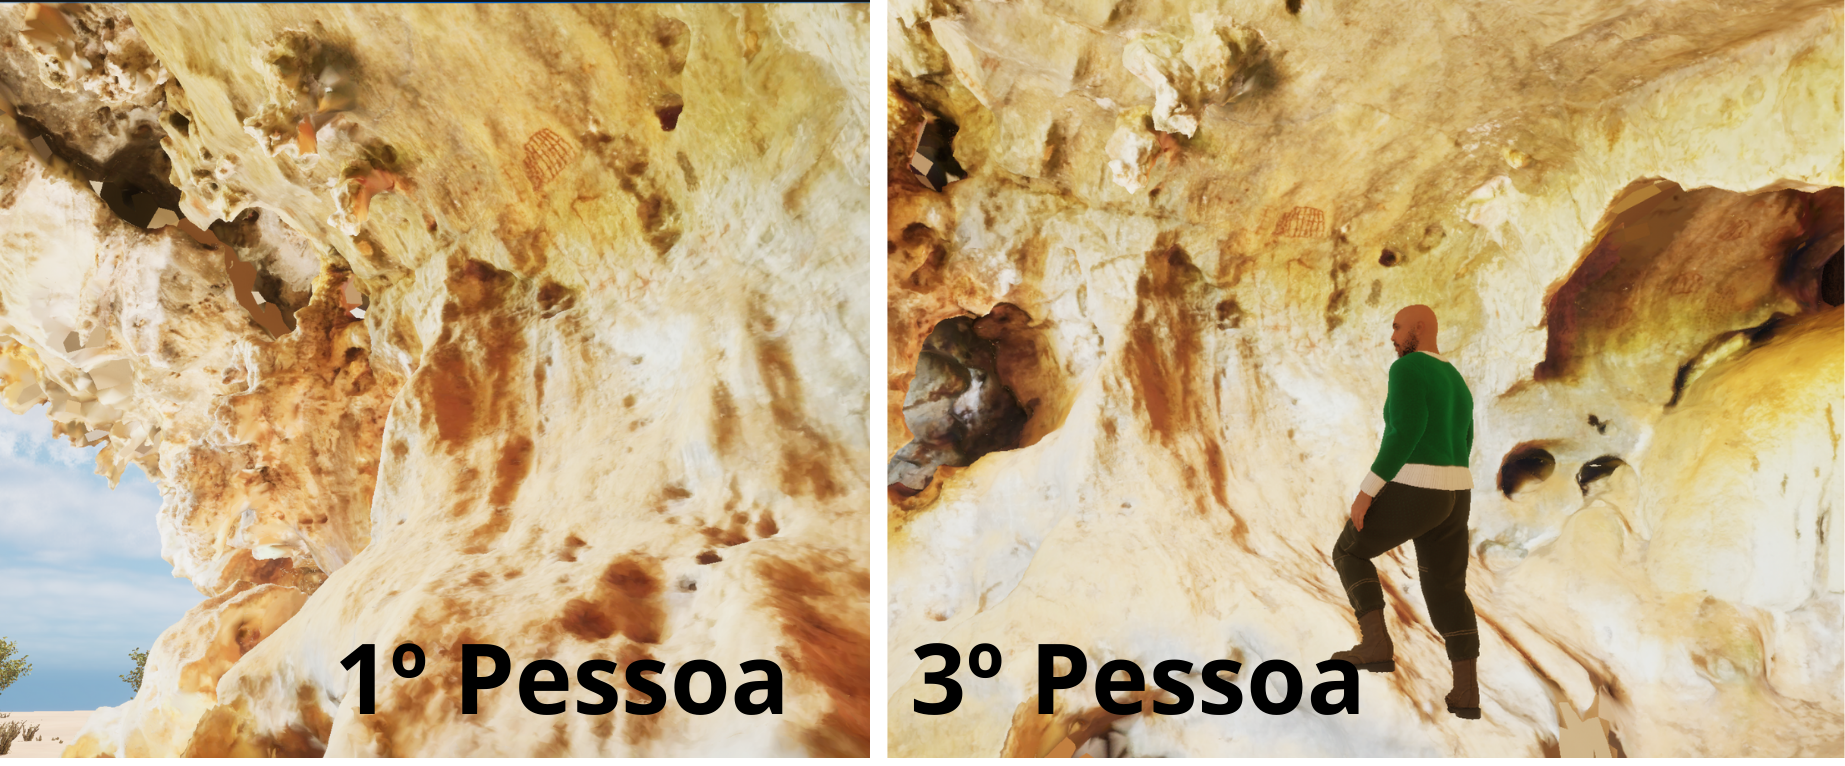
\includegraphics[height=6cm, keepaspectratio]{img/unreal/1 pessoa e 3 pessoa comparacao.png}
        \caption{Ajuste de posicionamento da câmera do avatar.
            \textbf{Fonte:} Elaborado pelo autor, 2025.}
        \label{fig:alternarcamera}
\end{figure}

\begin{figure}[H]
        \centering
        \includegraphics[height=8cm, keepaspectratio]{img/unreal/blueprint troca de câmera.png}
        \caption{Lógica da \textit{Blueprint} para troca de câmeras
            \textbf{Fonte:} Elaborado pelo autor, 2025.}
        \label{fig:blueprint_camera}
\end{figure}

\subsection{Criação de Tela de Menu}
Uma tela de menu inicial foi desenvolvida para facilitar a navegação e a interação do usuário. A tela inclui opções como iniciar o ambiente virtual, visitar o site, sair do aplicativo e descrição dos controles.
A interface foi projetada para ser intuitiva e esteticamente agradável, utilizando \textit{widgets}\footnote{Widgets são elementos de interação em interfaces gráficas, como janelas, botões e menus, que facilitam o acesso a aplicativos e ferramentas.} da \textit{Unreal Engine}. A Figura \ref{fig:tela_menu} mostra a tela de menu finalizada.

\begin{figure}[H]
        \centering
        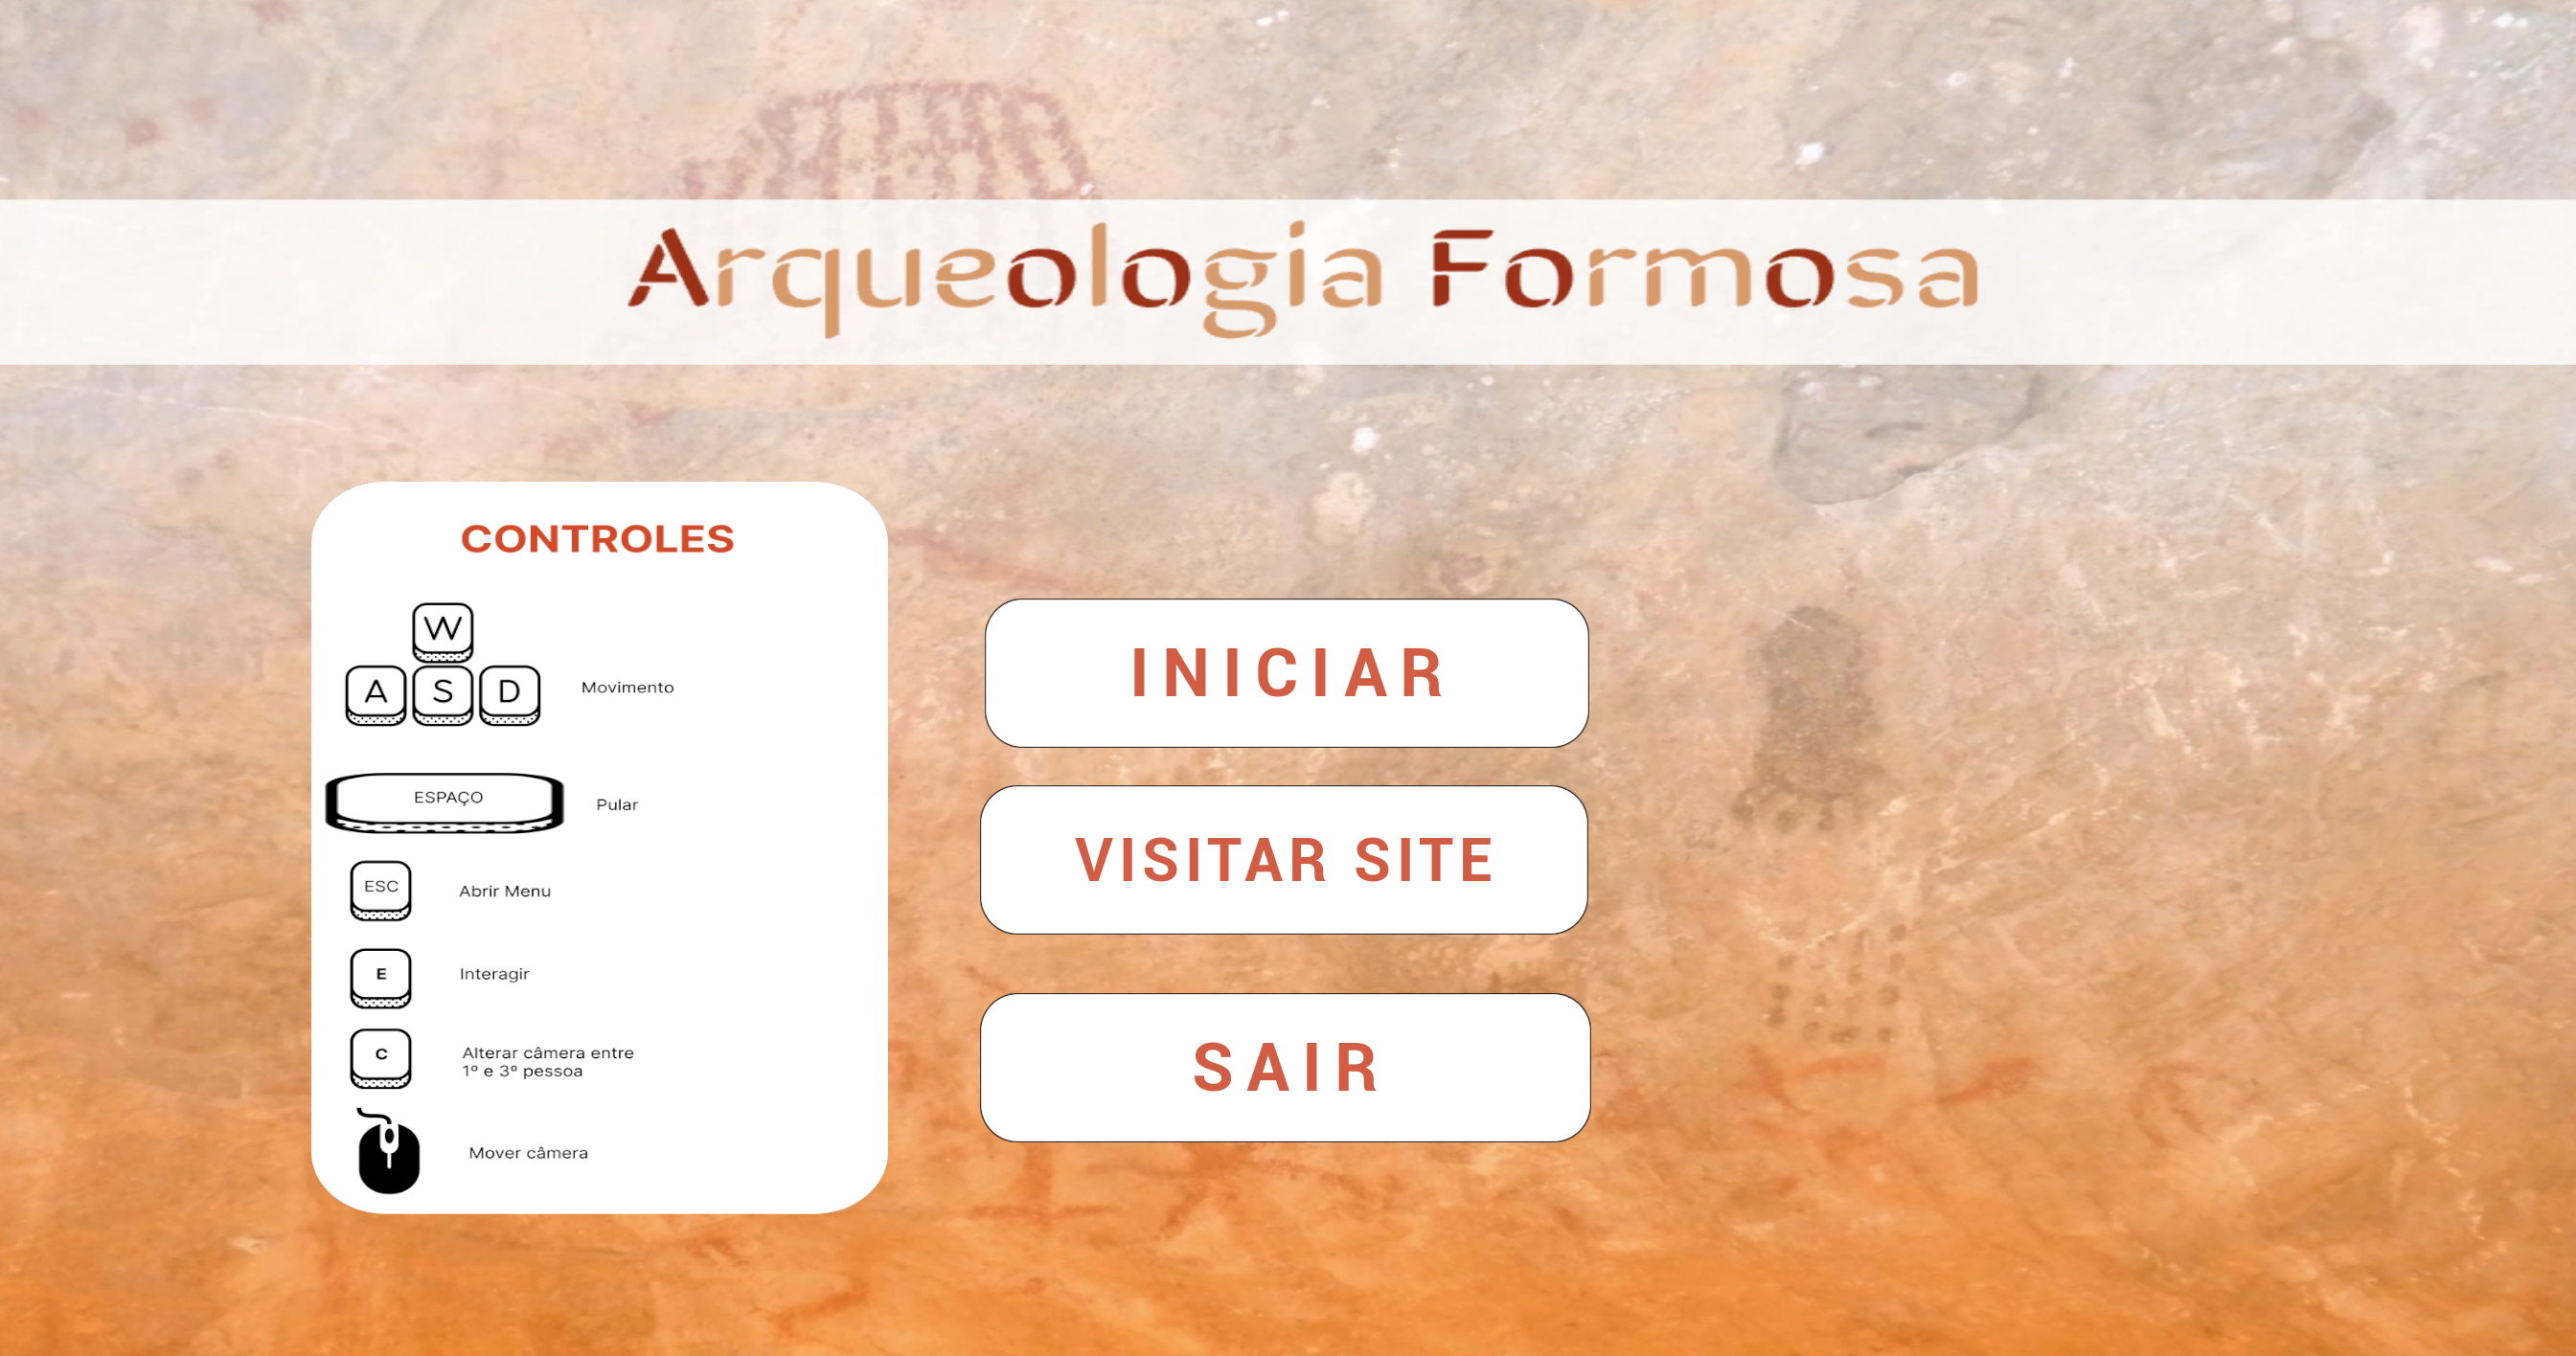
\includegraphics[height=8cm, keepaspectratio]{img/unreal/menu com controles.png}
        \caption{Tela de menu do ambiente virtual. \\
            \textbf{Fonte:} Elaborado pelo autor, 2025.}
        \label{fig:tela_menu}
\end{figure}


\subsection{Empacotamento do Ambiente Virtual e Criação de Instalador (RNFA003)}
O ambiente virtual foi empacotado em um arquivo executável (.exe) para distribuição. Para facilitar a instalação por usuários finais, foi criado um instalador utilizando o software \textit{Inno Setup}. A Figura \ref{fig:configuracao_inno_setup} representa a interface de desenvolvimento do instalador, que após configurado é compilado para ser executado em Windows.

\begin{figure}[H]
        \centering
        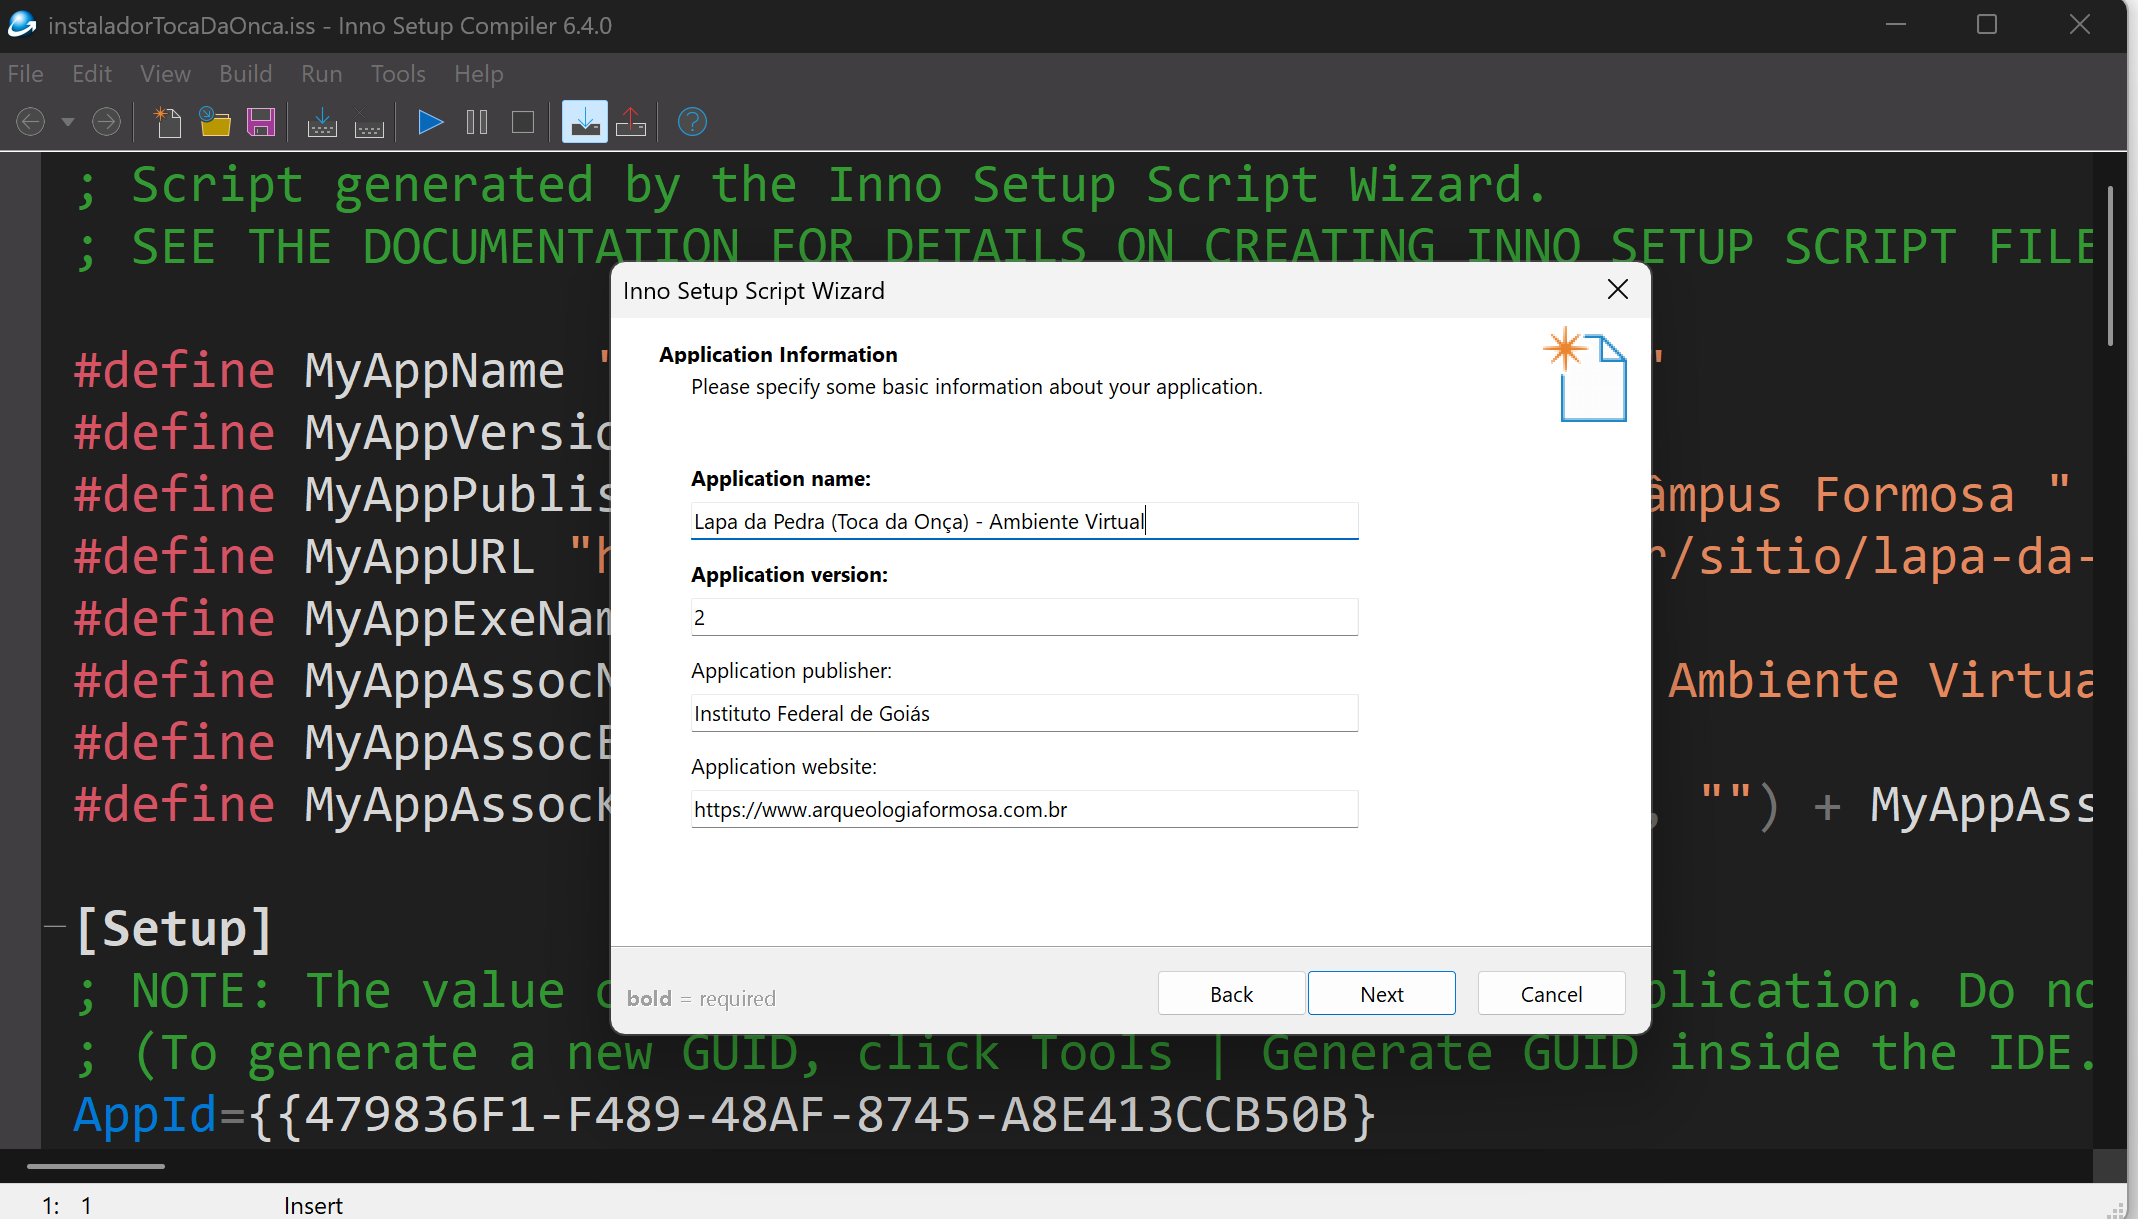
\includegraphics[height=8cm, keepaspectratio]{img/Inno setup/configuracao do instalador.png}
        \caption{Configurações iniciais para construir o instalador \\ na ferramenta Inno Setup \\
            \textbf{Fonte:} Elaborado pelo autor, 2025.}
        \label{fig:configuracao_inno_setup}
\end{figure}

Com o instalador criado basta dar um duplo clique no arquivo para começar o processo. O instalador inclui:
\begin{itemize}
    \item Suporte para instalação em múltiplos idiomas, demonstrado na Figura \ref{fig:idiomas};
    \begin{figure}[H]
        \centering
        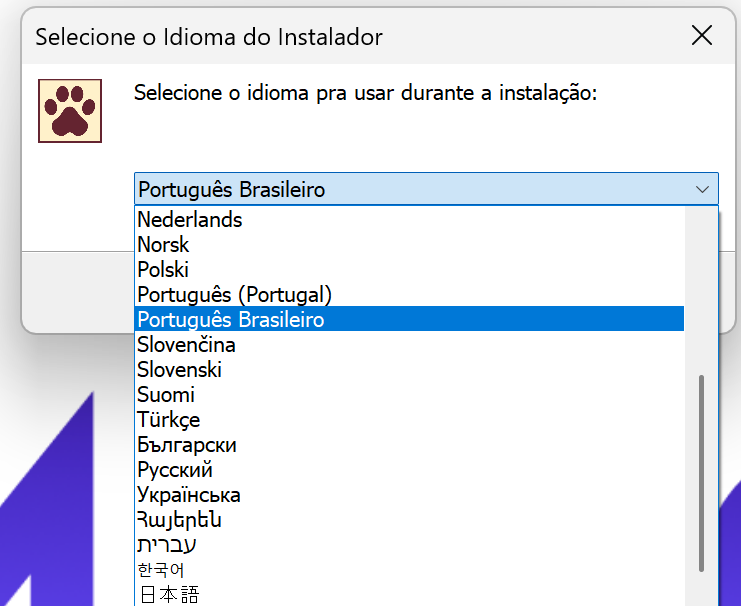
\includegraphics[height=8cm, keepaspectratio]{img/Inno setup/multiidiomas.png}
        \caption{Interface do instalador do ambiente virtual personalizado pelo \textit{Inno Setup }\\ com suporte a múltiplos idiomas \\
            \textbf{Fonte:} Elaborado pelo autor, 2025.}
        \label{fig:idiomas}
\end{figure}

    \item Interface simples e intuitiva, como demonstrado no fluxo de instalação da Figura \ref{fig:fluxo};
    \begin{figure}[H]
        \centering
        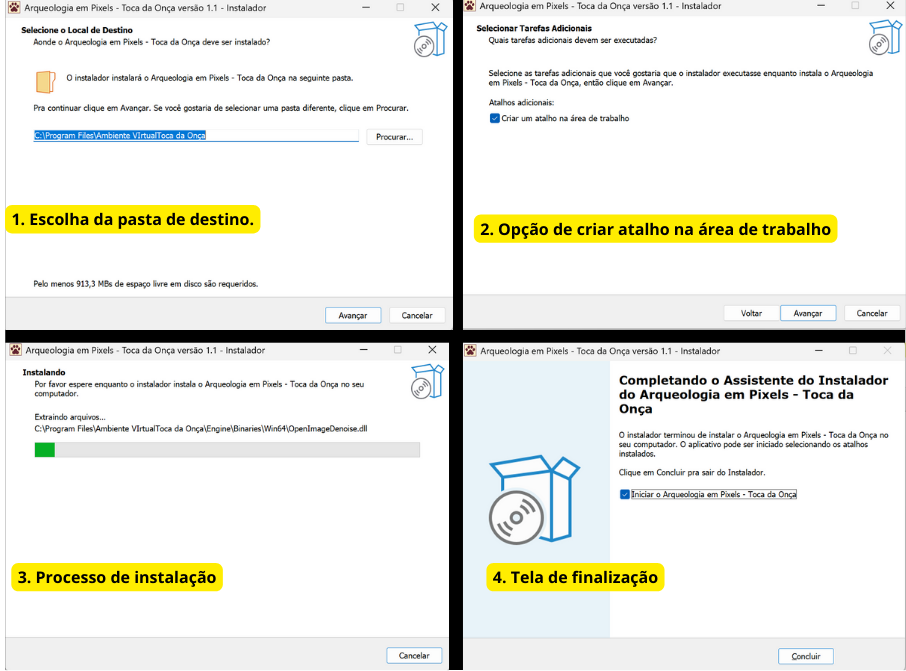
\includegraphics[height=12cm, keepaspectratio]{img/Inno setup/fluxo de instalação.png}
        \caption{Fluxo de instalação após a escolha do idioma. \\
            \textbf{Fonte:} Elaborado pelo autor, 2025.}
        \label{fig:fluxo}
\end{figure}

    \item Atalhos para a Área de Trabalho e Menu Iniciar (Figura \ref{fig:atalho_icone}). 
    \begin{figure}[H]
        \centering
        \includegraphics[height=8cm, keepaspectratio]{img/Inno setup/íconearea de trabalho.png}
        \caption{Atalho para o programa gerado na área de trabalho \\
            \textbf{Fonte:} Elaborado pelo autor, 2025.}
        \label{fig:atalho_icone}
\end{figure}
    
\end{itemize}




\subsection*{Considerações Finais do Ciclo 2}
O Ciclo 2 resultou na criação de um ambiente virtual interativo e imersivo, integrando o modelo 3D otimizado da Lapa da Pedra a um cenário rico e funcional na Unreal Engine 5.4. O ambiente virtual gerado nessa etapa está pronto para ser disponibilizado para distribuição no site que será construído nas etapas posteriores.



% Ciclo 3

% \textbf{Objetivo}: Criar um protótipo de alta fidelidade para o site.

% \textbf{Processo}:
% \begin{itemize}
%     \item Criação de uma identidade visual
%     \item Definição da arquitetura da informação e wireframes.
%     \item Desenvolvimento do protótipo no Figma.
%     \item Validação do design com stakeholders.
% \end{itemize}

\section{Ciclo 3: Prototipação do Novo Site}
\label{sec:ciclo3_site}

\textbf{Objetivo do Ciclo}: Desenvolver um protótipo o novo site, atendendo aos requisitos funcionais RFS002 (Exibir Galeria de Imagens), RFS006 (Buscar Trabalhos por Filtros) e RFS007 (Informações de Contato), bem como aos requisitos não funcionais RNFS006 (Acessibilidade), RNFS008 (Responsividade) e RNFS012 (SEO).

\subsection{Análise das Referências e Inspirações}
O processo teve início com uma análise detalhada das referências e inspirações fornecidas pelo professor Edson Borges por meio de entrevista e questionário, disponível no Apêndice \ref{ap:entrevista}. Essas referências incluíam exemplos de sites educacionais, culturais e interativos, que serviram como base para alinhar as expectativas e a visão do projeto. A análise permitiu identificar elementos-chave, como estilo visual minimalista e moderno, ênfase na acessibilidade e usabilidade, e coerência com a identidade cultural de páginas de Arqueologia. A Figura \ref{fig:inpirações} ilustra algumas das referências analisadas durante esta etapa, que foram colocadas lado a lado no Figma.

\begin{figure}[H]
    \centering
    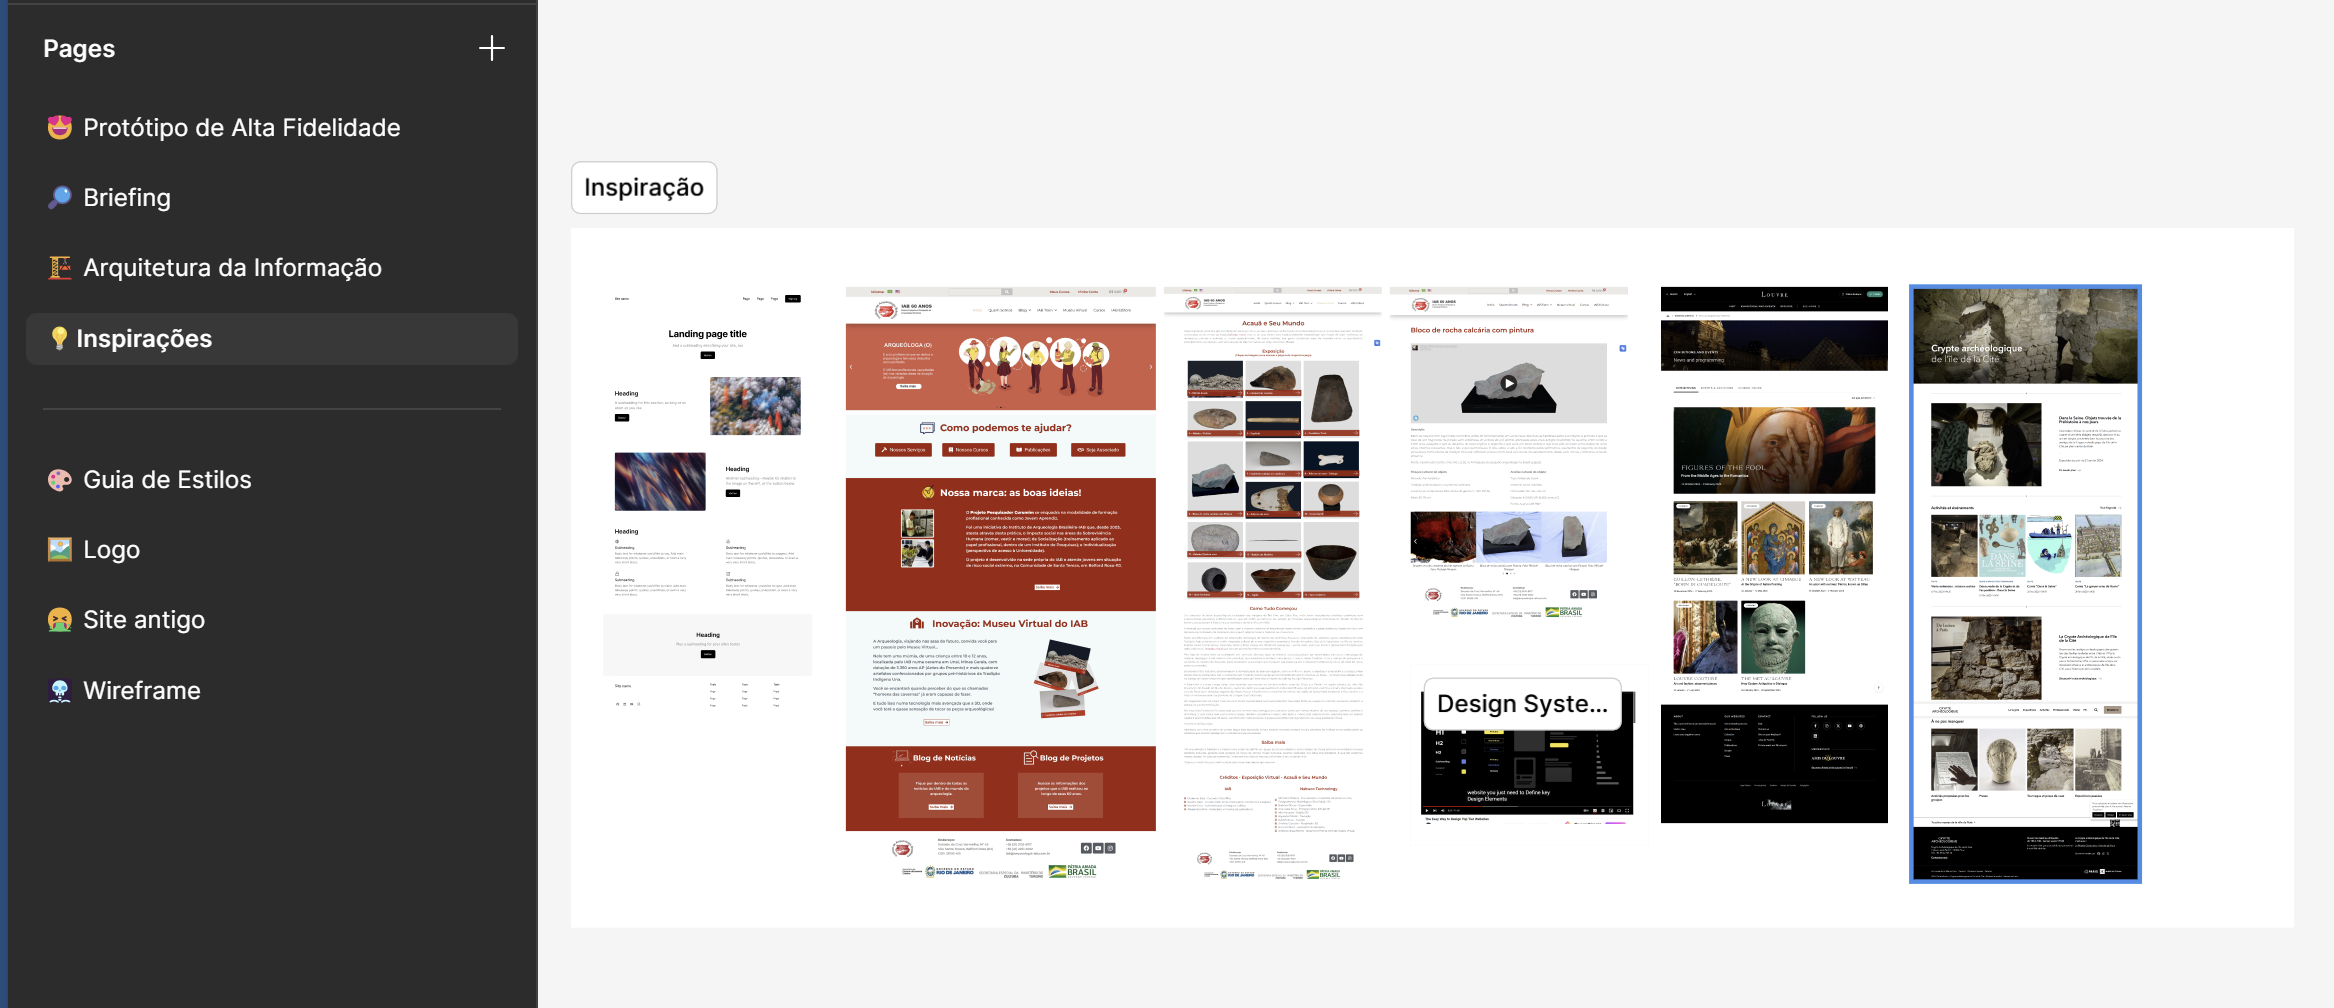
\includegraphics[height=6cm, keepaspectratio]{img/Protótipo/inspiração.png}
    \caption{ Inspirações de outros sites de Arqueologia, sites com boa estética, \\ paleta de cores ou forma atrativa. \\
        \textbf{Fonte:} Elaborado pelo autor, 2025.}
    \label{fig:inpirações}
\end{figure}

\subsection{Reorganização da Arquitetura da Informação}
Com base nas referências, foi realizada uma reorganização da arquitetura da informação do site, agrupando conteúdos relevantes, reduzindo informações desnecessárias e minimizando a quantidade de cliques necessários para que os usuários encontrassem as informações desejadas. Foi criada uma navegação hierárquica clara, com menus organizados por categorias principais, como "Página Inicial", "Sítios Arqueológicos", "Trabalhos Escritos", "Blog" e "Contato". Além disso, páginas secundárias foram eliminadas para evitar sobrecarga de conteúdo, e links rápidos foram adicionados para facilitar o acesso às principais funcionalidades do site, como o ambiente virtual e o download do instalador. Essas mudanças garantiram maior eficiência na navegação.

\subsection{Criação de Wireframes}
Para estruturar a interface do site, foram criados \textit{wireframes}\footnote{Wireframes são esboços visuais simplificados que representam a estrutura básica de uma interface, sem detalhes de design final, como cores ou imagens. Eles ajudam a planejar a disposição dos elementos na tela.} que definiram a disposição dos elementos visuais e interativos. Os \textit{wireframes} focaram em um layout responsivo, adaptável a diferentes dispositivos, como desktops, tablets e celulares, além de garantir um posicionamento estratégico de botões, menus e conteúdos prioritários. O espaçamento adequado entre os elementos foi planejado para facilitar a leitura e a interação. As Figuras \ref{fig:wireframes} e \ref{fig:wireframe} apresentam alguns dos \textit{wireframes} desenvolvidos durante esta fase.


\begin{figure}[H]
    \centering
    \begin{minipage}[b]{0.48\textwidth}
        \centering
        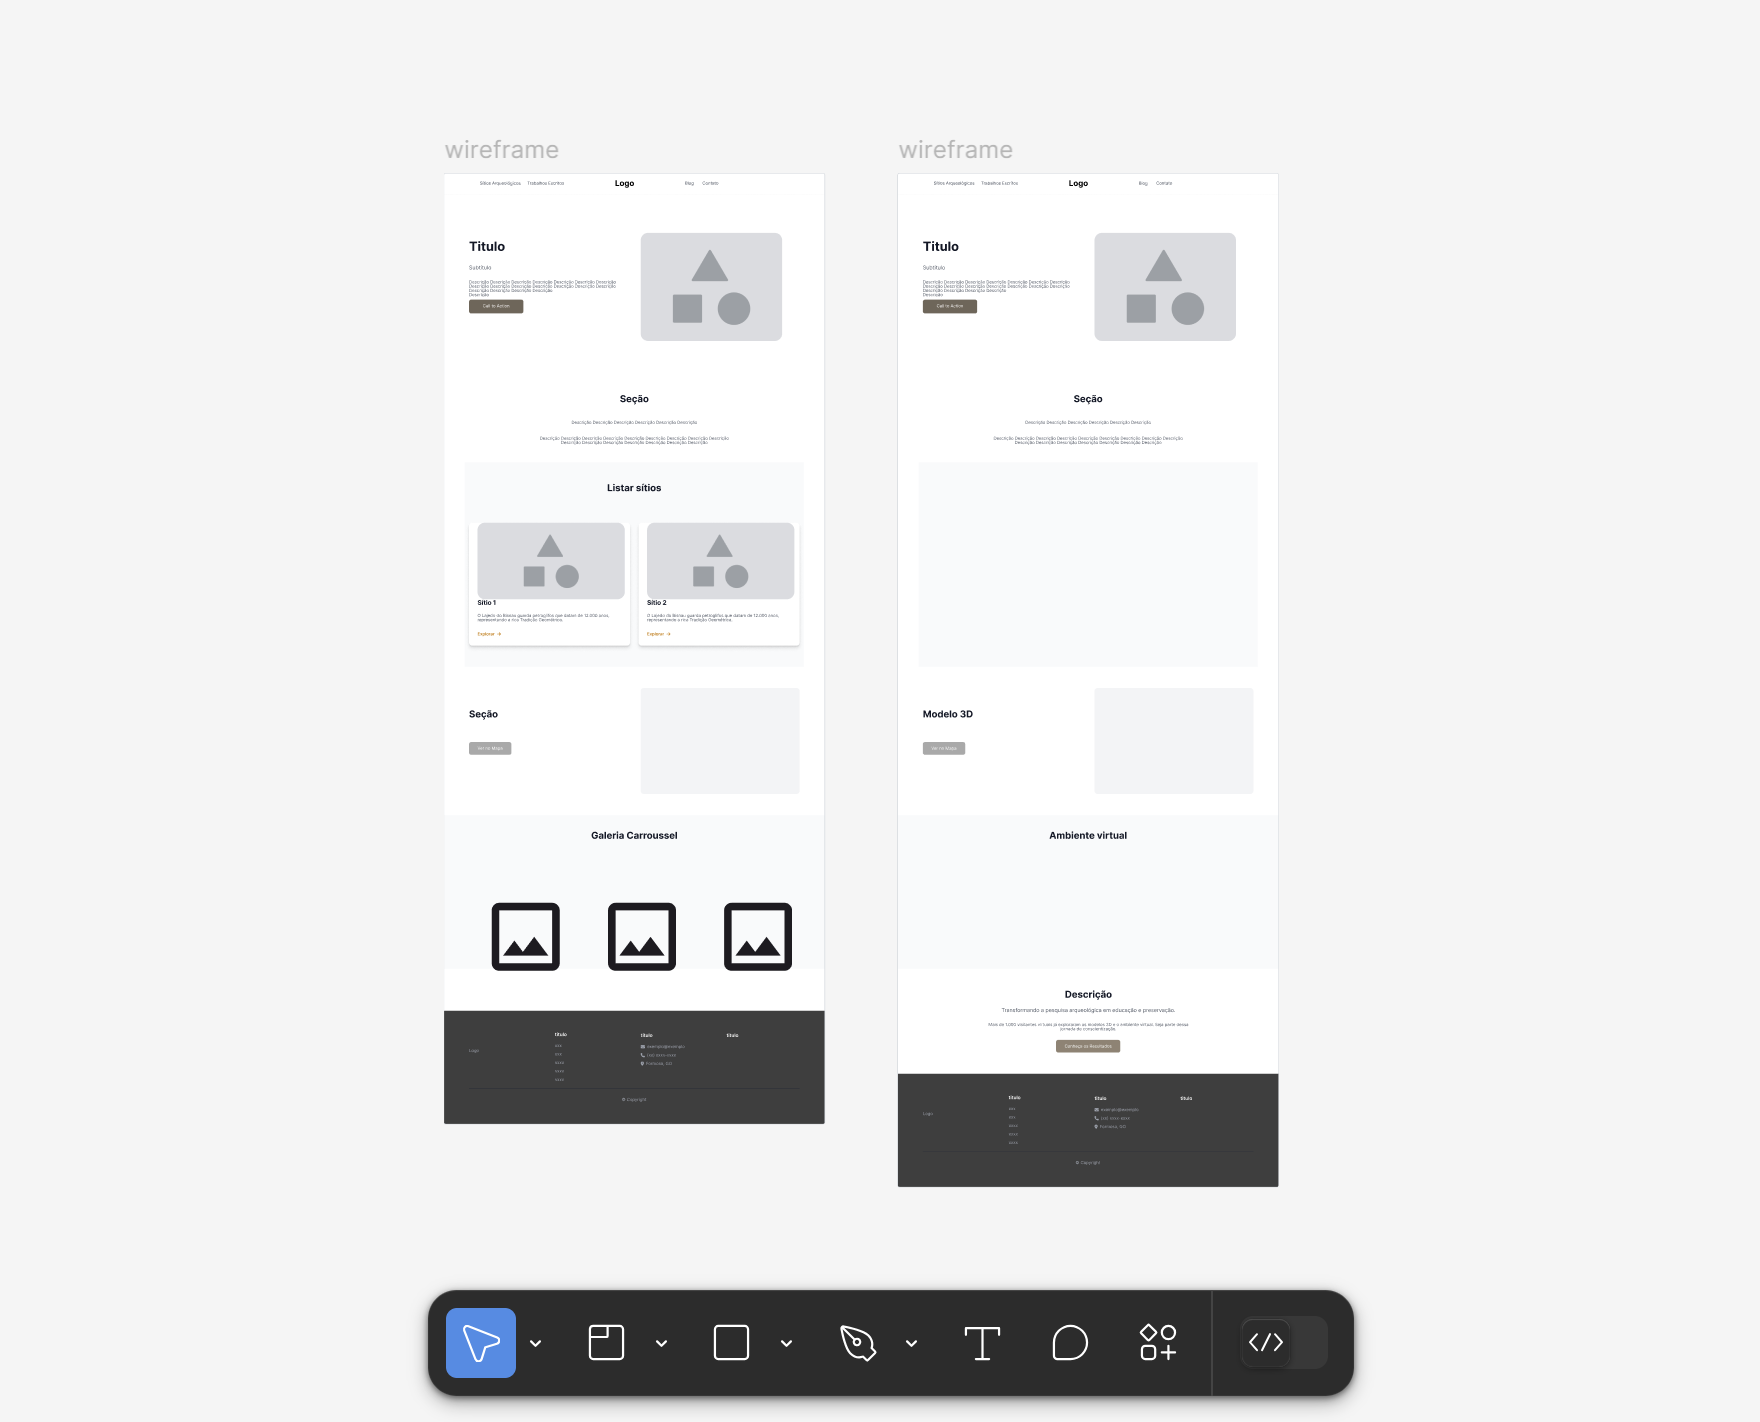
\includegraphics[height=8cm, keepaspectratio]{img/Protótipo/wireframes.png}
        \caption{Wireframes de baixa fidelidade \\no Figma. \\
            \textbf{Fonte:} Elaborado pelo autor, 2025.}
        \label{fig:wireframes}
    \end{minipage}
    \hfill
    \begin{minipage}[b]{0.48\textwidth}
        \centering
        \includegraphics[height=8cm, keepaspectratio]{img/Protótipo/wireframe.png}
        \caption{Wireframe de baixa fidelidade\\ no Figma ampliado. \\
            \textbf{Fonte:} Elaborado pelo autor, 2025.}
        \label{fig:wireframe}
    \end{minipage}
\end{figure}

% \subsection{Definição da Paleta de Cores e Tipografia}
% Foi definida uma paleta de cores e tipografia que refletisse a identidade visual do projeto com tons ocres, vermelhos, pretos, cinzas e brancos. Tons terrosos e verdes, inspirados nas cores das artes rupestres encontradas na Lapa da Pedra, foram escolhidos para compor a paleta de cores. Contrastes suficientes entre textos e fundos foram aplicados para atender aos critérios de acessibilidade, enquanto a fonte \textit{\textbf{Inter}} foi selecionada para melhorar a experiência de leitura. A Figura \ref{fig:paleta_cores} exibe a paleta de cores e exemplos de tipografia utilizados no projeto.

\subsection{Criação de uma Nova Logo}
Uma logo foi desenvolvida para o site, inspirada nas cores e formas das artes rupestres da Lapa da Pedra. A logo busca reforçar a identidade visual do projeto e estabelecer uma conexão direta com o tema arqueológico. A Figura \ref{fig:logo_arqueologia_formosa} mostra a logo finalizada.
\begin{figure}[H]
    \centering
    \includegraphics[height=8cm, keepaspectratio]{img/Protótipo/logo.png}
    \caption{ Logo do site Arqueologia Formosa inspirada nos pictoglifos e rochas da Lapa da Pedra. \\
        \textbf{Fonte:} Elaborado pelo autor, 2025.}
    \label{fig:logo_arqueologia_formosa}
\end{figure}


\subsection{Desenvolvimento do Protótipo de Alta Fidelidade}
Com base nos \textit{wireframes} e nas decisões de design, foram desenvolvidos protótipos de alta fidelidade no Figma para as principais telas (\ref{fig:prototipos_alta_fidelidade}). O protótipo representa a versão final do site, sendo que quando for transformado em código deve se assemelhar o máximo possível com o que foi prototipado. Foram feitos vários testes pedindo feedbacks de colegas, do orientador e do co-orientador. 

\begin{figure}[H]
    \centering
    \includegraphics[height=8cm, keepaspectratio]{img/Protótipo/todos alta fidelidade.png}
    \caption{ Protótipos de Alta Fidelidade das telas principais no Figma. \\
        \textbf{Fonte:} Elaborado pelo autor, 2025.}
    \label{fig:prototipos_alta_fidelidade}
\end{figure}

As Figuras \ref{fig:prototipo_home} e \ref{fig:prototipo_lapadapedra} apresentam o protótipo de alta fidelidade da Página Inicial e da Página do Sítio Arqueológico da Lapa da Pedra, respectivamente. 
% As demais telas do protótipo poderão ser vistas no Apêndice \ref{ap:prototipos}.

\begin{figure}[H]
    \centering
    \begin{minipage}[b]{0.48\textwidth}
        \centering
        \includegraphics[height=24cm, keepaspectratio]{img/Protótipo/home prototipo.png}
        \caption{Protótipo de alta fidelidade da página inicial. \\
            \textbf{Fonte:} Elaborado pelo autor, 2025.}
        \label{fig:prototipo_home}
    \end{minipage}
    \hfill
    \begin{minipage}[b]{0.48\textwidth}
        \centering
        \includegraphics[height=24cm, keepaspectratio]{img/Protótipo/prototipo alta fidelidade toca da onça.png}
        \caption{Protótipo de alta fidelidade \\da página do Sítio Arqueológico da Lapa da Pedra \\
            \textbf{Fonte:} Elaborado pelo autor, 2025.}
        \label{fig:prototipo_lapadapedra}
    \end{minipage}
\end{figure}

\subsection*{Considerações Finais do Ciclo 3}
O Ciclo 3 resultou no desenvolvimento de um protótipo de alta fidelidade para o novo site.O design final segue bons princípios de design, as heurísticas de Nielsen e é alinhado com a identidade cultural do projeto. O protótipo está pronto para implementação e servirá como base para a construção do site final, que é o próximo ciclo. 

% Ciclo 4
\section{Ciclo 4: Desenvolvimento do Novo Site}
\label{sec:ciclo4_desenvolvimento}

O objetivo deste ciclo é implementar o a interface e as funcionalidades planejadas no protótipo feito no ciclo anterior, buscando atender aos requisitos funcionais e não funcionais do site. O desenvolvimento abrange a maioria dos requisitos especificados nas tabelas \ref{ap:requisitos-site-table} e \ref{ap:requisitos-nao-funcionais-site-table}, garantindo acessibilidade (RNFS006), responsividade (RNFS008), gerenciamento dinâmico de conteúdo (RFS009) e otimização de desempenho (RNFS001, RNFS011).

    \subsection{Configuração do Ambiente de Desenvolvimento e Arquitetura}
     Foi definida a arquitetura \textit{JAMstack}. A Figura \ref{fig:arquitetura arqueologia formosa} apresenta uma visão geral dos componentes da arquitetura e suas interações. O \textit{framework} \textit{Next.js 15} é utilizado no \textit{front-end} para garantir alta performance e SEO (RNFS012), sendo responsável pela geração do site estático e otimização do código. Suas principais funcionalidades incluem Geração Estática Incremental (ISR) para atualização eficiente do conteúdo.
     Para o gerenciamento de conteúdo, foi utilizado o \textit{Sanity}, um CMS headless que permite a criação e manutenção de conteúdo de forma dinâmica e flexível (RFS009). A biblioteca \textit{Schema UI} foi integrada para facilitar a construção de componentes reutilizáveis e consistentes. 
     
     Além disso, foi configurado um repositório no \textit{Github} para controle de versão e armazenamento do código-fonte. O repositório \textit{git} está acessível em \href{https://github.com/Takeshi-mi/arqueologiaFormosa}{https://github.com/Takeshi-mi/arqueologiaFormosa}. 
     A infraestrutura é baseada em serviços \textit{cloud}, sendo a \textit{Vercel} para hospedagem e CDN, que oferece otimização automática de desempenho, alta disponibilidade, baixa latência e redução de custos operacionais (RNFS011);
     E serviços \textit{cloud} como \textit{Google Drive} e \textit{Dropbox} para o armazenamento de arquivos grandes (modelos 3D, ambiente virtual, PDFs).

     O fluxo de dados no sistema segue um padrão unidirecional: editores atualizam o conteúdo através da interface do Sanity CMS, alterações disparam \textit{webhooks} que iniciam o processo de \textit{build}, \textit{Next.js} gera novas páginas estáticas incorporando o conteúdo atualizado e \textit{Vercel} realiza o \textit{deploy} automático e distribui o conteúdo através de sua rede CDN. O mesmo processo acontece quando o código armazenado no \textit{Github} é atualizado.

    \begin{figure}[H]
        \centering
        \includegraphics[height=16cm, keepaspectratio]{img/arquitetura/arquitetura-arqueologia-formosa.png}
        \caption{ Diagrama da arquitetura do sistema. \\
            \textbf{Fonte:} Elaborado pelo autor, 2025.}
        \label{fig:arquitetura arqueologia formosa}
    \end{figure}
    
    \subsection{Estrutura da Base de Dados no Sanity}
     O \textit{Sanity} utiliza um modelo \textit{NoSQL}\footnote{NoSQL é uma sigla que significa "não apenas SQL" e se refere a um tipo de banco de dados que não usa tabelas relacionais. Em vez disso, os bancos de dados NoSQL armazenam dados em formatos como documentos, grafos, colunas ou chave-valor.} para armazenamento de dados, permitindo flexibilidade na definição de esquemas (\textit{schemas}) e relacionamentos entre documentos. A Figura \ref{fig:diagrama sanity} apresenta a representação da base de dados.

    \begin{figure}[H]
        \centering
        \includegraphics[height=20cm, keepaspectratio]{img/sanity/upscalemedia-transformed.png}
        \caption{ Representação da base de dados não relacional do site.\\
            \textbf{Fonte:} Elaborado pelo autor, 2025.}
        \label{fig:diagrama sanity}
    \end{figure}

    \subsubsection{Integração do Sanity com os Componentes}
    No \textit{Sanity}, um componente funcional depende de três elementos essenciais: o \textit{\textbf{schema}}, que define a estrutura dos dados e garante a consistência do conteúdo; a \textit{\textbf{query}}\footnote{Uma query é um pedido de uma informação ou de um dado. Esse pedido também pode ser entendido como uma consulta, uma solicitação ou, ainda, uma requisição.}, escrita em GROQ\footnote{GROQ: Linguagem de consulta desenvolvida pelo \textit{Sanity} para recuperar e manipular dados de forma eficiente em bancos NoSQL, permitindo filtrar, ordenar e estruturar informações conforme necessário.}, que recupera os dados do \textit{back-end} de forma eficiente e os disponibiliza para uso; e o \textbf{código do componente}, responsável por transformar esses dados em uma interface visual e interativa.
    Para facilitar, existe a biblioteca \href{https://schemaui.com/docs/}{Schema UI}, que desempenhou um papel relevante no processo de desenvolvimento ao agilizar a criação e personalização de interfaces no \textit{Sanity}. Ela disponibiliza um conjunto de componentes pré-construídos, que podem ser utilizados diretamente ou adaptados para atender às necessidades específicas do projeto. Esses componentes simplificam a implementação do código do componente , permitindo que o foco seja direcionado à personalização visual e funcional, sem a necessidade de criar soluções do zero. Nos casos em que os componentes fornecidos pela biblioteca não atenderam as necessidades do projeto, foram criados componentes personalizados, como foi o caso do componente estilizado para aceitar \textit{embed}\footnote{O elemento\textit{ <embed>} na linguagem de marcação HTML é utilizado para incorporar conteúdo externo, como arquivos de áudio, vídeo e mapas, diretamente em uma página web. Ele permite que aplicativos externos sejam integrados no documento, possibilitando a reprodução de mídia sem a necessidade de abrir um site separado.} para adicionar conteúdos de sites externos, como os mapas e modelos 3D diretamente na tela. A Figura \ref{fig:schemaui} apresenta um exemplo da documentação do \textit{Schema UI}, exemplificando o uso dos três elementos essenciais para que um componente integrado com \textit{Sanity} funcione corretamente.

\begin{figure}[H]
    \centering
    \includegraphics[height=24cm, keepaspectratio]{img/shcema ui qualidade.png}
    \caption{ Captura de tela da documentação do \textit{Schema UI} do componente de cartão "GRID POST". \\
        \textbf{Fonte:} Elaborado pelo autor com base na documentação da biblioteca \href{https://schemaui.com/docs/components/grid/grid-post}{Schema UI}, 2025.}
    \label{fig:schemaui}
\end{figure}



    \subsection{Estrutura de Pastas no Next.js} O projeto foi organizado em uma estrutura de pastas clara e modular, seguindo as boas práticas do Next.js. A Figura \ref{fig:estrutura_pastas} apresenta a estrutura de diretórios. Essa organização facilita a manutenção do código e a implementação de novas funcionalidades (RNFS004).

\begin{figure}[H]
    \centering
    \includegraphics[height=18cm, keepaspectratio]{img/site/estrutura de diretórios.png}
    \caption{ Estrutura de diretórios do projeto em Next.js. \\
        \textbf{Fonte:} Elaborado pelo autor, 2025.}
    \label{fig:estrutura_pastas}
\end{figure}

    \subsection{Implementação da estrutura e funcionalidades do site}
    Com tudo preparado era hora de estilizar e povoar o site com as informações e identidade visual planejada.
    \begin{enumerate}
        \item \textbf{Implementação de páginas-chave}:
        \begin{enumerate}
            \item Página inicial com navegação hierárquica, garantindo fácil acesso às principais seções do site (RFS006, RNFS014);
            \item Seções específicas para sítios arqueológicos, incluindo galerias de imagens (RFS002) e mapa interativo personalizado com a localização dos sítios integrados ao \textit{Google My Maps}\footnote{É uma ferramenta do Google Permite a criação, edição e compartilhamento de mapas personalizados online.} (RFS012);
            \item Página de Contato, com formulário funcional e informações de contato visíveis (RFS007);
            \item Página de trabalhos escritos com filtros dinâmicos, permitindo busca por categorias e tags (RFS006);
            \end{enumerate}
            Todas as páginas podem ser vistas no Apêndice \ref{apendice paginas site}.

            As páginas também tem a sua versão responsiva para dispositivos móveis, atendendo ao requisito não funcional RNF008 (Responsividade), conforme mostrado nas Figuras \ref{fig:menu hamburguer}, e \ref{fig:menu mobile}, demonstrando como o menu se adaptou. 

    \begin{figure}[H]
    \centering
    % Primeira figura
    \begin{minipage}{0.45\textwidth} % Reduzi a largura para 45%
        \centering
    \includegraphics[height=8cm, keepaspectratio]{img/site/menu hamburguer lateral.png}
    \caption{ Interface responsiva para dispositivos móveis.\\ A seta indica o ícone de menu hambúrguer, \\uma boa prática para adaptar o menu à telas menores.\\
        \textbf{Fonte:} Elaborado pelo autor, 2025.}
    \label{fig:menu hamburguer}   
    \end{minipage}
    \hspace{1cm} % Espaço fixo de 0.5cm entre as figuras
    % Segunda figura
    \begin{minipage}{0.45\textwidth} % Reduzi a largura para 45%
        \centering
        \includegraphics[height=8cm, keepaspectratio]{img/site/menu mobile.png}
        \caption{Menu hambúrguer expandido.\\
            \textbf{Fonte:} Elaborado pelo autor, 2025.}
        \label{fig:menu mobile}
    \end{minipage}
\end{figure}

            
        \item \textbf{Implementação das funcionalidades}:
            \begin{enumerate}
            \item Adição de suporte para modo escuro/claro (RNFS011), permitindo alternância entre temas com base nas preferências do usuário (Figura \ref{fig:claro escuro};

                    \begin{figure}[H]
                        \centering
                        \includegraphics[height=7cm, keepaspectratio]{img/site/claro escuro.png}
                        \caption{ Funcionalidade modo claro/escuro. \\
                            \textbf{Fonte:} Elaborado pelo autor, 2025.}
                        \label{fig:claro escuro}
                    \end{figure}
                                
            \item Integração com o \textit{Sanity Studio} que atua como uma área do administrador para gerenciamento dinâmico de conteúdo, como artigos, imagens e metadados (RFS009, RNFS013). A interface de administrador é demonstrada na Figura \ref{fig:sanity_admin};

                    \begin{figure}[H]
                        \centering
                        \includegraphics[height=9cm, keepaspectratio]{img/sanity/sanity admin.png}
                        \caption{ Interface de edição do Sanity Studio. \\
                            \textbf{Fonte:} Elaborado pelo autor, 2025.}
                        \label{fig:sanity_admin}
                    \end{figure}
                    
        Para acessar essa parte do sistema é necessário que o usuário esteja autenticado (RFS08,RNF005). Utilizando \textit{Sanity}, já vem configurado por padrão as opções de \textit{login} com o \textit{Google}, \textit{Github} ou E-mail/senha.
        \begin{figure}[H]
    \centering
    \includegraphics[height=8cm, keepaspectratio]{img/site/login.png}
    \caption{Página de Login para acesso da área administrativa. \\
    \textbf{Fonte:} Elaborado pelo autor, 2025.}
    \label{fig:footer}
\end{figure}
            \item Implementação de funcionalidades de compartilhamento nas redes sociais (RFS005), demosntrado na Figura \ref{fig:redes sociais}
                    \begin{figure}[H]
                        \centering
                        \includegraphics[height=8cm, keepaspectratio]{img/site/redes sociais.png}
                        \caption{ Opção de compartilhar trabalho escrito nas redes sociais. \\
                            \textbf{Fonte:} Elaborado pelo autor, 2025.}
                        \label{fig:redes sociais}
                    \end{figure}
        \end{enumerate}
    \end{enumerate}
        


\subsubsection*{Considerações Finais do Ciclo 4}
O Ciclo 4 resultou no desenvolvimento completo do site, atendendo plenamente aos requisitos funcionais e não funcionais estabelecidos. A arquitetura \textit{JAMstack}, combinada com o uso do \textit{Next.js} e \textit{Sanity}, garantiu um sistema robusto, escalável e de alto desempenho. O código Até essa etapa o site foi desenvolvido em ambiente local. Nas próximas etapas serão detalhados os processos de testes e disponibilização para o público.





% avaliacao
\section{Avaliação e Testes}
\label{sec:avaliacao_testes}

Para garantir que a solução atenda aos requisitos definidos foram realizados testes de usabilidade, com usuários clicando e testando as funcionalidades e verificando se estavam de acordo com o que foi planejado e com auxílio de análise heurística.

Também foi verificada a performance e acessibilidade do site por meio da ferramenta \textit{Lighthouse}. Os resultados dos testes estão apresentados no Capítulo \ref{cap:resultados}.
O site foi testado em 6 navegadores diferentes para verificar a compatibilidade. Os navegadores foram: \textit{Microsoft Edge, Google Chrome, Opera GX, Firefox, Brave, e Safari}.

Foi produzido um plano de testes detalhado que não foi implementado completamente, mas pode servir como direcionamento futuro. O plano de testes está no Apêndice \ref{ap:plano de testes}.

% Deploy
\section{Publicação e Deploy}
\label{sec:publicacao_deploy}

Está foi uma fase importante para tornar o projeto acessível ao público. A seguir é detalhado o processo, que envolveu:

\begin{itemize}
    \item Hospedagem\footnote{Hospedagem é o serviço que disponibiliza os recursos necessários (como servidores e infraestrutura) para armazenar e entregar um site ou aplicação na internet.} e \textit{deploy}\footnote{Deploy é o processo de colocar uma aplicação ou site em produção, tornando-o acessível aos usuários finais, geralmente envolvendo a transferência de código para um ambiente de hospedagem.} na Vercel (Figura \ref{fig:deploy_vercel}). 
\begin{figure}[H]
    \centering
    \includegraphics[height=8cm, keepaspectratio]{img/Deploy/deploy_vercel.png}
    \caption{ Captura de tela do processo de deploy na vercel. \\
        \textbf{Fonte:} Elaborado pelo autor, 2025.}
    \label{fig:deploy_vercel}
\end{figure}

    \item Registro de domínio pelo \href{www.registro.br}{Registro.br}, que é o departamento do NIC.br responsável pelas atividades de registro e manutenção dos nomes de domínios que usam o .br. Essa escolha garante maior confiabilidade, identidade nacional e melhor indexação nos mecanismos de busca (Figura \ref{fig:dominio_registro_br}).
\begin{figure}[H]
    \centering
    \includegraphics[height=8cm, keepaspectratio]{img/Deploy/domínio-registro.br.png}
    \caption{ Domínio disponível para compra no site \href{www.registro.br}{Registro.br}. \\
        \textbf{Fonte:} Elaborado pelo autor, 2025.}
    \label{fig:dominio_registro_br}
\end{figure}

    \item Configuração de DNS para apontar o domínio para a \textit{Vercel} (Figura \ref{fig:dns}).
\begin{figure}[H]
    \centering
    \includegraphics[height=8cm, keepaspectratio]{img/Deploy/configuração de dns registrobr.png}
    \caption{ Configuração de DNS para apontar o domínio para a \textit{Vercel}. \\
        \textbf{Fonte:} Elaborado pelo autor, 2025.}
    \label{fig:dns}
\end{figure}

\end{itemize}




 \chapter{Resultados}
\label{cap:resultados}

O objetivo geral deste trabalho foi plenamente alcançado com a criação de uma plataforma digital que une um site moderno e um ambiente virtual 3D, ambos voltados para a preservação, divulgação e democratização do acesso à arte rupestre da cidade de Formosa, Goiás. O novo site apresenta um design responsivo, organização clara das informações e funcionalidades como galeria de imagens e acesso a modelos 3D, enquanto o ambiente virtual proporciona uma imersão detalhada nas pinturas rupestres, permitindo exploração interativa e download para uso offline. Essa solução não apenas resolve os problemas de usabilidade e acessibilidade identificados no site anterior, mas também promove a conscientização sobre a importância desses registros culturais, alinhando-se ao propósito de preservar e valorizar o patrimônio arqueológico da região de Formosa.
As seções a seguir detalham como os objetivos específicos foram atendidos.

\s\ection{Análise Heurística de Usabilidade: Problemas Identificados no Site Antigo}
Um dos objetivos específicos era realizar uma análise heurística de usabilidade do antigo site "Arqueologia Formosa". Essa análise foi conduzida com base nas heurísticas de Nielsen, avaliando aspectos como navegabilidade, eficiência e consistência. Os principais problemas identificados foram:
\begin{itemize}
    \item Layout desorganizado, dificultando a localização de informações importantes.
    \item Falta de responsividade para dispositivos móveis.
    \item Ausência de funcionalidades modernas, como busca por filtros e visualização do modelo 3D dentro do próprio site.
\end{itemize}

Esses problemas foram utilizados como base para o planejamento do novo site, garantindo que as falhas do sistema anterior fossem corrigidas. A análise heurística também guiou a priorização das melhorias implementadas.

\section{Implementação de um Ambiente Virtual \gls{3d}}
Outro objetivo específico era implementar um ambiente virtual \gls{3d} que permitisse a visualização interativa da arte rupestre. Esse objetivo foi alcançado com o desenvolvimento de um ambiente imersivo na Unreal Engine, utilizando modelos \gls{3d} gerados por fotogrametria. Os resultados incluem:
\begin{itemize}
    \item Fidelidade visual dos modelos \gls{3d} gerados por fotogrametria, com texturas realistas das pinturas rupestres;
    \item Navegação interativa no ambiente, permitindo aos usuários explorar o sítio arqueológico em primeira e terceira pessoa;
    \item Avatar personalizado baseado no professor Edson Borges;
    \item Empacotamento do ambiente virtual em um arquivo executável, disponibilizado para \textit{download} no site.
\end{itemize}

A Figura \ref{fig:virtual_environment} apresenta uma visão do ambiente virtual desenvolvido.

\begin{figure}[H]
    \centering
    % Substitua pelo caminho do arquivo de imagem
    \includegraphics[width=0.8\linewidth]{img/unreal/Captura de tela 2025-02-12 125127.png}
    \caption{Ambiente virtual desenvolvido na Unreal Engine.}
    \label{fig:virtual_environment}
\end{figure}

\section{Desenvolvimento de um Novo Site com Design Centrado no Usuário (\gls{ux})}
O novo site foi desenvolvido com tecnologias modernas (\textit{Next.js}, \textit{Tailwind CSS} e \textit{Sanity CMS}), priorizando uma experiência do usuário intuitiva e acessível. Os resultados alcançados incluem:
\begin{itemize}
    \item Design responsivo, otimizado para dispositivos móveis, desktops e tablets.
    \item Galeria de imagens organizada, com suporte para visualização ampliada.
    \item Modo escuro/claro, permitindo maior conforto visual.
    \item Implementação de padrões de acessibilidade conforme WCAG 2.1 (nível AA).
\end{itemize}

A Figura \ref{fig:site_homepage} apresenta a página inicial do novo site, evidenciando o layout moderno e a organização do conteúdo.

\begin{figure}[H]
    \centering
    \includegraphics[height=6cm, keepaspectratio]{img/site/hero1.png}
    \caption{Página inicial do novo site "Arqueologia Formosa". \\
    \textbf{Fonte:} Elaborado pelo autor, 2025.}
    \label{fig:site_homepage}
\end{figure}

As demais páginas podem ser vista no Apêndice \ref{ap:páginas_do_site} e no site publicado na internet, acessível por meio do endereço \url{www.arqueologiaformosa.com.br}.

\section{Testes e Validação}
Para comprovar a qualidade do produto desenvovido foram realizados alguns testes. Os resultados desses testes estão descritos abaixo:
% \subsection{Usabilidade}
% Os testes de usabilidade foram realizados com base nas heurísticas de Nielsen. Os seguintes pontos foram avaliados:
% \begin{itemize}
%     \item Facilidade de navegação no site e no ambiente virtual.
%     \item Eficiência na interação com a galeria de imagens e o ambiente virtual.
%     \item Satisfação dos usuários com o design e as funcionalidades implementadas.
% \end{itemize}


% \begin{table}[H]
% \centering
% \caption{Resultados dos testes de usabilidade.}
% \label{tab:usabilidade}
% \begin{tabularx}{\textwidth}{|l|X|X|} % Ajusta a largura da tabela ao texto
% \hline
% \textbf{Critério Avaliado} & \textbf{Pontuação Média} & \textbf{Observações} \\ \hline
% Facilidade de Navegação    & 4.7/5                   & Navegação intuitiva e bem estruturada. \\ \hline
% Interação com o Conteúdo    & 4.6/5                   & Boa experiência na galeria de imagens e no ambiente virtual. \\ \hline
% Design e Funcionalidades    & 4.8/5                   & Alta satisfação com o layout moderno e intuitivo. \\ \hline
% \end{tabularx}
% \end{table}
\begin{enumerate}

\item{Desempenho}
Os testes de desempenho foram realizados com o \textit{Google Lighthouse}. Abaixo estão os principais resultados:
\begin{table}[H]
\centering
\caption{Resultados dos testes de desempenho realizados com o \textit{Google Lighthouse}.}
\label{tab:desempenho}
\begin{tabularx}{\textwidth}{|l|X|} % Ajusta a largura da tabela ao texto
\hline
\textbf{Critério Avaliado} & \textbf{Resultado} \\ \hline
Tempo de carregamento médio & 1 segundo \\ \hline
Tempo até o primeiro conteúdo visível aparecer & 0,8 segundos \\ \hline
Pontuação em SEO & 100/100 \\ \hline
Pontuação em Desempenho & 95/100 \\ \hline
Responsividade & Boa responsividade em dispositivos móveis e desktops \\ \hline
\end{tabularx}
\end{table}
As Figuras \ref{fig:lighthouse} e \ref{fig:tempocarregamento} mostram capturas de tela dos testes realizados com a ferramenta \textit{Google Lighthouse}.
\begin{figure}[H]
    \centering
    \includegraphics[height=6cm, keepaspectratio]{img/site/lighthouse_only.png}
    \caption{Análise de desempenho do site Arqueologia Formosa pela ferramenta \textit{Lighthouse}. \\
    \textbf{Fonte:} Elaborado pelo autor, 2025.}
    \label{fig:lighthouse}
\end{figure}

\begin{figure}[H]
    \centering
    \includegraphics[height=6cm, keepaspectratio]{img/site/tempo_de_carregamento.png}
    \caption{Tempo de carregamento da página medido pelo \textit{Lighthouse}. \\
    \textbf{Fonte:} Elaborado pelo autor, 2025.}
    \label{fig:tempocarregamento}
\end{figure}

\item{Acessibilidade}
O site final seguiu as regras de conformidade com as diretrizes WCAG 2.1, e foram medidas com testes de usabilidade e teste de contraste feitas no site \href{https://dequeuniversity.com/rules/axe/4.10/color-contrast}{\textit{Deque University - Color Contrast}}. Foram garantidos o contraste adequado para textos e botões (Figura \ref{fig:testeconstraste}); a navegação por teclado funcionando corretamente; e a compatibilidade com leitores de tela. O leitor de tela utilizado para os testes foi o \href{https://www.tcees.tc.br/acessibilidade/leitor-de-tela-nvda/}{NVDA}\footnote{NVDA é um programa de código aberto para leitura de tela que permite que pessoas cegas ou com deficiência visual acessem e interajam com o sistema através de voz sintética.}. Além disso o site alcançou uma pontuação de 91/100 em acessibilidade utilizando a ferramenta \textit{Lighthouse}, como mostrado na Figura \ref{fig:lighthouse}

\begin{figure}[H]
    \centering
    \includegraphics[height=6cm, keepaspectratio]{img/site/contraste.png}
    \caption{Teste de constraste de acordo com o \\ padrão WCAG medido pela ferramenta de contraste da \href{https://dequeuniversity.com/rules/axe/4.10/color-contrast}{\textit{Deque University}}. \\
    \textbf{Fonte:} Elaborado pelo autor, 2025.}
    \label{fig:testeconstraste}
\end{figure}

\end{enumerate}


\chapter{Considerações Finais} \label{cap:Considerações Finais}

Este trabalho demonstrou como tecnologias digitais inovadoras podem ser aplicadas à preservação e divulgação do patrimônio arqueológico, especificamente das pinturas rupestres do sítio Lapa da Pedra, em Formosa-GO. 
Cumpriram-se os objetivos do trabalho ao desenvolver uma plataforma digital que combina um site moderno e um ambiente virtual imersivo para a Lapa da Pedra. Conforme demonstrado nos Resultados (Seção \ref{cap:resultados}). O novo site atingiu ótimas métricas em usabilidade, desempenho e acessibilidade e o ambiente virtual permitiu uma exploração detalhada das pinturas rupestres.
A implementação deste trabalho não apenas cumpriu o objetivo proposto, mas também abriu portas para novas formas de educação patrimonial.

\section{Limitações e Dificuldades}
\label{sec:limitações}
Durante o desenvolvimento, algumas dificuldades foram enfrentadas, como por exemplo:
\begin{itemize}
    \item Dificuldades na otimização dos modelos 3D para uso na Unreal Engine;
    \item Limitação de tempo para implementar todas as funcionalidades desejadas;
    \item Restrições no orçamento;
    \item Limitações hardware para produzir os modelos 3D e o ambiente virtual na Unreal. Houveram processos que demoraram mais de 30 horas para renderizar;
    \item Compatibilidade: O ambiente virtual não foi testado em hardware muito antigo, restringindo o acesso a usuários com computadores básicos.
\end{itemize}

\section{Trabalhos Futuros} \label{sec:futuro}

Para expandir o projeto, diversas melhorias e novas funcionalidades podem ser implementadas. Uma sugestão é a integração com Realidade Virtual (VR), adicionando suporte para headsets como \textit{Oculus Rift} ou \textit{Meta Quest}, o que permitiria uma imersão total no ambiente virtual, proporcionando uma experiência mais envolvente para os usuários. Além disso, seria interessante desenvolver uma versão mobile do projeto, com um aplicativo para Android e iOS que ofereça recursos simplificados de visualização 3D, tornando o conteúdo acessível a um público ainda maior.
Outra possibilidade seria incorporar modelos 3D de outros sítios arqueológicos, utilizando a mesma infraestrutura já desenvolvida. Também se pode considerar a implementação de um chatbot com inteligência artificial no site, capaz de interagir com os visitantes e fornecer informações detalhadas sobre os sítios arqueológicos e o patrimônio cultural.


\subsection{Contribuição para a Área}
Este trabalho contribuiu para a interseção entre Arqueologia e tecnologia ao oferecer um modelo replicável para digitalização de sítios arqueológicos em regiões subrepresentadas e ao promover a conscientização sobre a importância da preservação cultural através de ferramentas acessíveis.

\subsection{Palavras Finais}
A preservação do patrimônio arqueológico é um desafio árduo e contínuo. Espera-se que esta iniciativa inspire novas pesquisas e políticas públicas voltadas à proteção digital de nossa herança cultural. 

% Referências
\begin{references}
\bibliography{bib/references}
\end{references}

% Apêndices
\theappendix
\chapter{Requisitos do Ambiente Virtual}\label{apendice}
% No Apêndice

\section{Requisitos Funcionais do Ambiente Virtual}\label{ap:requisitos-ambiente-table}
\begin{longtable}{|l|l|p{6cm}|l|}
    \caption{Requisitos Funcionais do Ambiente Virtual}
    \label{tab:requisitos-funcionais-ambiente}
    \hline
    \textbf{ID} & \textbf{Nome} & \textbf{Descrição} & \textbf{Prioridade} \\ \hline
    \endfirsthead
    \hline
    \textbf{ID} & \textbf{Nome} & \textbf{Descrição} & \textbf{Prioridade} \\ \hline
    \endhead
    RFA001 & Modelo 3D de Alta Qualidade & Modelo 3D gerado via fotogrametria, compatível com Unreal Engine 5.4. & Essencial \\ \hline
    RFA002 & Navegação em Terceira Pessoa & Controle de um avatar com movimentação livre pelo ambiente (andar, correr, saltar). & Essencial \\ \hline
    RFA003 & Alternância de Câmera & Opção de alternar entre visão em primeira e terceira pessoa durante a navegação. & Importante \\ \hline
    RFA004 & Avatar Personalizado & Customização do Avatar semelhante ao professor. & Desejável \\ \hline
\end{longtable}

\section{Requisitos Não Funcionais do Ambiente Virtual}\label{ap:requisitos-nao-funcionais-ambiente}
\begin{longtable}{|l|l|p{6cm}|l|}
    \caption{Requisitos Não Funcionais do Ambiente Virtual}
    \label{tab:requisitos-nao-funcionais-ambiente}
    \hline
    \textbf{ID} & \textbf{Nome} & \textbf{Descrição} & \textbf{Prioridade} \\ \hline
    \endfirsthead
    \hline
    \textbf{ID} & \textbf{Nome} & \textbf{Descrição} & \textbf{Prioridade} \\ \hline
    \endhead
    RNFA001 & Compatibilidade com Windows & O ambiente virtual deve ser executável em Windows 10 ou superior. & Essencial \\ \hline
    RNFA002 & Instalação Simplificada & O ambiente virtual deve ser empacotado em alguma ferramenta de instalação, como o Inno Setup, que permita a distribuição simplificada e organizada para os usuários finais. & Importante \\ \hline
\end{longtable}

\chapter{Requisitos do Site} \label{Apendice B}

\vspace{1cm}
\section{Requisitos Funcionais do Site}\label{ap:requisitos-site-table}
{\small % Reduz o tamanho da fonte para economizar espaço
\begin{longtable}{|>{\raggedright}p{2.5cm}|>{\raggedright}p{4cm}|p{6cm}|>{\raggedright}p{2cm}|}
\caption{Requisitos Funcionais do Site}
\hline
\textbf{Identificador} & \textbf{Nome} & \textbf{Descrição} & \textbf{Prioridade} \\
\hline
\endfirsthead % Cabeçalho da primeira página
\hline
\textbf{Identificador} & \textbf{Nome} & \textbf{Descrição} & \textbf{Prioridade} \\
\hline
\endhead % Cabeçalho das páginas seguintes
RFS001 & Publicar Trabalhos Escritos & Permitir a publicação de artigos, relatórios de PIBIC, e-books e outras produções acadêmicas, organizados por categorias e tags. & Essencial \\
\hline
RFS002 & Exibir Galeria de Imagens & Oferecer uma galeria de imagens relacionada aos sítios arqueológicos, com suporte para visualização ampliada. & Importante \\
\hline
RFS003 & Baixar Modelos 3D & Oferecer a opção de download de modelos 3D do sítio arqueológico. & Essencial \\
\hline
RFS004 & Ambiente Virtual para Download & Disponibilizar o arquivo executável do ambiente virtual desenvolvido na Unreal Engine para download pelos usuários. & Essencial \\
\hline
RFS005 & Compartilhar nas Redes Sociais & Permitir o compartilhamento de conteúdos e links diretamente no WhatsApp e E-mail. & Desejável \\
\hline
RFS006 & Buscar Trabalhos por Filtros & Oferecer um mecanismo de busca que permita filtrar trabalhos escritos por categorias e por sítios arqueológicos. & Desejável \\
\hline
RFS007 & Informações de Contato & Disponibilizar informações de contato como telefone e email para que os usuários possam entrar em contato com os administradores do sistema. & Importante \\
\hline
RFS008 & Autenticação de Usuário & Implementar autenticação de usuário, diferenciando permissões entre administradores e leitores. & Essencial \\
\hline
RFS009 & Gerenciamento de Conteúdo & Permitir que administradores adicionem, editem ou removam postagens e outros conteúdos diretamente no sistema. & Essencial \\
\hline
RFS010 & Alterar Layout do Site & Administradores devem poder modificar o layout do site, sem a necessidade de programação. & Desejável \\
\hline
RFS011 & Modo Escuro/Claro & Oferecer uma alternância entre modos escuro e claro para a interface. & Desejável \\
\hline
RFS012 & Exibir Mapa dos Sítios Arqueológicos & Exibir mapas interativos, integrados ao Google Maps, para a localização dos sítios arqueológicos. & Importante \\
\hline
RFS013 & Monitoramento de Acessos & Integrar ferramentas como Google Analytics para coletar dados sobre o número de acessos e comportamento dos usuários no site. & Importante \\
\hline
\end{longtable}
} % Fim do ambiente \small



\section{Requisitos Não Funcionais do site}

{\small % Reduz o tamanho da fonte para economizar espaço
\begin{longtable}{|>{\raggedright}p{2.5cm}|>{\raggedright}p{4cm}|p{6cm}|>{\raggedright}p{2cm}|}
\caption{Tabela de Requisitos Não Funcionais}
\label{ap:requisitos-nao-funcionais-site-table}
\hline
\textbf{Identificador} & \textbf{Nome} & \textbf{Descrição} & \textbf{Prioridade} \\
\hline
\endfirsthead % Cabeçalho da primeira página
\hline
\textbf{Identificador} & \textbf{Nome} & \textbf{Descrição} & \textbf{Prioridade} \\
\hline
\endhead % Cabeçalho das páginas seguintes
RNFS001 & Tempo de Carregamento & O sistema deve carregar as páginas em até 3 segundos em uma conexão de 5 Mbps. & Essencial \\
\hline
RNFS002 & Performance Visível & As páginas principais devem exibir conteúdo visível para o usuário em até 2 segundos após o carregamento inicial. Deve atingir pelo menos 80/100 de pontuação em performance no Lighthouse. & Essencial \\
\hline
RNFS003 & Escalabilidade & O sistema suportar até 10.000 visitantes simultâneos sem perdas expressivas na performance.  & Importante \\
\hline
RNFS004 & Manutenibilidade & O código do sistema deve ser modular e seguir boas práticas de desenvolvimento, facilitando atualizações e correções futuras. & Importante \\
\hline
RNFS005 & Segurança & O sistema deve garantir a segurança dos dados por meio de HTTPS, e deve garantir a autenticação segura de usuários por meio de provedores \textit{Single Sign-On} (SSO) confiáveis, como o Google, com proteção contra acesso não autorizado.  & Essencial \\
\hline
RNFS006 & Acessibilidade & O site deve seguir as diretrizes WCAG 2.1 (nível AA), garantindo suporte a leitores de tela, navegação por teclado e contraste adequado. Deve atingir pelo menos 80/100 de pontuação em acessibilidade no Lighthouse. & Importante \\
\hline
RNFS007 & Compatibilidade com Navegadores & O sistema deve ser compatível com os navegadores mais utilizados (Google Chrome, Firefox, Safari e Edge) em suas versões mais recentes. & Importante \\
\hline
RNFS008 & Responsividade & O site deve ser responsivo, oferecendo uma experiência adequada em dispositivos móveis, tablets e desktops. & Essencial \\
\hline
RNFS009 & Confiabilidade & O sistema deve ter uma disponibilidade mínima de 99,9\% mensal. & Essencial \\
\hline
RNFS010 & Tolerância a Falhas & O sistema deve implementar backups para garantir a recuperação de dados em caso de falhas. & Importante \\
\hline
RNFS011 & Custos Operacionais Reduzidos & O sistema deve ser projetado para funcionar com ferramentas e serviços gratuitos sempre que possível, reduzindo custos operacionais. & Desejável \\
\hline
RNFS012 & SEO (Otimização para Motores de Busca) & O sistema deve ser otimizado para SEO, garantindo que o conteúdo seja facilmente encontrado em mecanismos de busca como Google. & Importante \\
\hline
RNFS013 & Integração com Serviços Externos & O sistema deve permitir integração fluida com plataformas como Sanity (CMS), Google Maps, Flickr e Google Drive. & Essencial \\
\hline
\end{longtable}
} % Fim do ambiente \small

\chapter{Entrevista}\label{ap:entrevista}

O conteúdo abaixo é fruto de adaptações de um questionário feito no Google Forms e entrevistas orais realizadas pelo estudante Erik Takeshi Miura para o professor Edson Borges.


\begin{enumerate}
    \item \textbf{Qual é o objetivo principal do site reformulado?}  
    Divulgação dos resultados obtidos com as pesquisas já realizadas (e as futuras) sobre os sítios arqueológicos de Formosa.  
    Permitir que as pessoas acessem informações, relatórios, resultados, imagens, modelos 3D, ambiente virtual, relatórios e publicações.

    \item \textbf{Quem é o público-alvo do site?}  
    Pesquisadores/as, interessados/as em arqueologia, estudantes, turistas e demais pessoas interessadas.

    \item \textbf{Qual mensagem ou impressão o site deve transmitir?}  
    Transmitir a necessidade de estudo e preservação do patrimônio arqueológico da cidade de Formosa.  
    O site deve passar uma impressão de seriedade e sobriedade.

    \item \textbf{O conteúdo atual será mantido, atualizado ou substituído?}  
    Sim, o conteúdo atual será mantido, com atualizações e edições.

    \item \textbf{Quais tipos de conteúdo devem receber destaque no novo site?}  
    Imagens, modelos interativos e produção bibliográfica.

    \item \textbf{Há necessidade de novas seções ou categorias no site? Se sim, quais?}  
    Sim, mas ainda não foram definidas quais seções ou categorias serão criadas.

    \item \textbf{Quais problemas de design no site atual mais incomodam?}  
    Navegação, acessibilidade, inclusão, layout e diagramação são problemas atuais.  
    \textbf{Feedback recebido:} Usuários relataram dificuldade em encontrar informações devido ao site estar muito carregado e com seções bagunçadas.

    \item \textbf{Já foi recebido feedback dos usuários sobre o site atual? Se sim, qual?}  
    Sim. O feedback recebido foi que os usuários não conseguiram encontrar o que procuravam devido ao site estar muito carregado e com seções desorganizadas.

    \item \textbf{Existem sites ou referências visuais que servem como inspiração? Se sim, quais?}  
    Sim, os seguintes sites foram citados como referência:  
    \begin{itemize}
        \item \url{https://arqueologia-iab.com.br/}  
        \item \url{https://www.espacoarqueologia.com.br/}  
        \item \url{https://arqueologiaeprehistoria.com/o-que-e-arqueologia/}  
        \item \url{https://www.crypte.paris.fr/}  
        \item \url{https://www.louvre.fr/en/online-tours}  
        \item \url{https://www.japanhousesp.com.br/exposicao/nihoncha-introducao-ao-cha-japones/}
    \end{itemize}

    \item \textbf{Há uma paleta de cores ou identidade visual que deve ser seguida?}  
    Sim. A paleta de cores inclui tons ocres, vermelhos, pretos, cinzas e brancos.

    \item \textbf{Quais funcionalidades o site deve ter?}  
    \begin{itemize}
        \item Barra de busca  
        \item Botão de compartilhamento em redes sociais  
        \item Galeria de imagens  
        \item Integração com vídeos do YouTube ou Vimeo  
        \item Monitoramento de tráfego (ex.: Google Analytics)  
        \item Formulário para contato  
        \item Download de conteúdo (Modelos 3D, imagens, livros, simulações, etc.)  
        \item Ambiente virtual (não é uma plataforma de jogo, mas um ambiente interativo)  
        \item Outras funcionalidades que a imaginação permitir
    \end{itemize}

    \item \textbf{Será necessária autenticação de usuários?}  
    Sim, será necessária. Só pessoas com acesso podem modificar o site. Tem que ter uma área de administrador pra gerenciar o conteúdo.

    \item \textbf{Como podemos facilitar o acesso às informações para os usuários?}  
    Ampliação da divulgação e uso de palavras-chave adequadas para facilitar o acesso.  
    Melhorar a organização do conteúdo para evitar sobrecarga e confusão nas seções.

    \item \textbf{O site precisa ser acessível para pessoas com deficiência?}  
    Sim, o site precisa ser acessível para pessoas com deficiência.

    \item \textbf{Quais dispositivos e navegadores o público-alvo mais utiliza?}  
    Computadores desktop e smartphones.

    \item \textbf{Quem será responsável por atualizar o site no futuro?}  
    O cliente será responsável por atualizar o site no futuro.

    \item \textbf{Há necessidade de um sistema de gerenciamento de conteúdo (CMS)?}  
    Sim, há necessidade de um CMS.

    \item \textbf{Qual é a frequência esperada de atualizações no site?}  
    Provavelmente uma vez por ano, que é o tempo de um novo relatório de PIBIC ser publicado.

    \item \textbf{Existe alguma tecnologia ou ferramenta preferida para o desenvolvimento do site?}  
    Plataformas que possibilitem o uso de modelos 3D e ambiente virtual, como Unreal Engine ou outras.

    \item \textbf{Há necessidade de integração com outras plataformas? Se sim, quais?}  
    Não há necessidade de integração com outras plataformas.

    \item \textbf{Qual é o orçamento disponível para a manutenção e hospedagem do site a longo prazo?}  
    Não há orçamento definido, mas será avaliado o que é possível fazer. O orçamento é bastante restrito.

    \item \textbf{Como saberemos que o site reformulado está cumprindo seu objetivo?}  
    Creio que podemos deixar um pedido de avaliação da visitação, ou acompanhar os acessos.

    \item \textbf{Quais métricas ou indicadores de desempenho devem ser acompanhados?}  
    Contador de visitas (atualmente, o site tem cerca de 900 visualizações por ano, com 70 visualizações por mês).  
    Aumento de acessos pode ser esperado com divulgação em redes de ensino e turismo.
\end{enumerate}



% \chapter{Protótipos}\label{prototipos}
% \label{ap:prototipos}

\begin{figure}[H]
    \centering
    \includegraphics[height=8cm, keepaspectratio]{img/Protótipo/todos alta fidelidade.png}
    \caption{ Protótipos de Alta Fidelidade das telas principais no Figma. \\
        \textbf{Fonte:} Elaborado pelo autor, 2024.}
    \label{fig:prototipo_alta_fidelidade}
\end{figure}

\chapter{Páginas do Site}\label{apendice paginas site}
\input{appendix/Páginas_do_site}\label{ap:páginas_do_site}

\chapter{Plano de testes}\label{ap:plano de testes}
Esse documento de plano de testes foi desenvolvido, mas não implementado completamente. Ele pode ser utilizado como um direcionamento futuro.
\includepdf[pages=-]{appendix/planotestes.pdf}
\end{document}
